%--------------------------------------------------------------------------
\chapter{Group Actions}
\label{app:group-actions}

%--------------------------------------------------------------------------
\begin{definition}
	\cite[99]{Rotman1967}
	\cite[41]{DummitFoote2004}
	Let $X$ be a set and $G$ a group. An \textbf{action} of $G$ on $X$ is a function
	$G \times X \to X$ given by $(g, x) \mapsto gx$, such that:
	\begin{enumerate}
		\item $(gh)x = g(hx)$ for all $g, h \in G$ and $x \in X$;
		\item $1x = x$ for all $x \in X$, where $1 \in G$ is the identity.
	\end{enumerate}
\end{definition}

%--------------------------------------------------------------------------
\begin{proposition}
	\cite[99]{Rotman1967}
	\cite[42]{DummitFoote2004}
	If a group $G$ acts on a set $X$ then, for every $g \in G$, the function
	$f_g : X \to X$ given by $f_g(x) = gx$ is a permutation of $X$. Further, the function
	$f : G \to S_X$ given by $f(g) = f_g$ is a homomorphism and, conversely, for any
	homomorphism $\phi : G \to S_X$, there is a corresponding group action given by
	$\phi(g)(x)$.
\end{proposition}

%--------------------------------------------------------------------------
\begin{theorem}[Cayley]
	\cite[96]{Rotman1967}
	\cite[120]{DummitFoote2004}
	Every group is isomorphic to a subgroup of the symmetric group $S_G$. In particular,
	if $|G| = n$, then $G$ is isomorphic to a subgroup of $S_n$.
\end{theorem}

%--------------------------------------------------------------------------
\begin{theorem}
	\cite[97]{Rotman1967}
	Let $H \leq G$ be a subgroup of finite index $n$. Then there exists a homomorphism
	$\phi : G \to S_n$ such that $\ker \phi \leq H$. In particular, when $H = \{ 1 \}$,
	this is Cayley's theorem.
\end{theorem}

%--------------------------------------------------------------------------
\begin{example}
	\cite[122]{DummitFoote2004}
	A group acts on itself by conjugation. Let $g, h \in G$ and $x \in G$. Then
	$1 x 1^{-1} = x$ and
	\begin{equation}
		g(hx) = g(h x h^{-1}) = gh x h^{-1}g^{-1} = (gh) x (gh)^{-1} = (gh)x \enspace.
	\end{equation}
	It is also immediate from the above that a group acts on its power set by conjugation.
	In particular, a group acts on the set of all its subgroups.
\end{example}

%--------------------------------------------------------------------------
\begin{definition}
	\cite[100]{Rotman1967}
	\cite[112]{DummitFoote2004}
	If $G$ acts on $X$, then the \textbf{orbit} of $x \in X$ is the set
	\begin{equation}
		\mathcal{O}(x) = \{ gx : g \in G \} \subseteq X \enspace.
	\end{equation}
	An action is \textbf{transitive} if there is only one orbit. The \textbf{kernel}
	of the action is the set
	\begin{equation}
		\{ g \in g : gx = x, \forall x \in X \} \enspace.
	\end{equation}
	An action is \textbf{faithful} if the kernel is the identity. The
	\textbf{stabilizer} of $x$ in $G$ is the group
	\begin{equation}
		G_x = \{ g \in g : gx = x \} \leq G \enspace.
	\end{equation}
	When a group acts on itself by conjugation, the orbits are called
	\textbf{conjugacy classes}. The stabilizer of some $g \in G$ is the
	\textbf{centralizer} of $g$ in $G$, denoted $C_G(g)$. When a group acts on the set of
	its subgroups by conjugation, the stabilizer of a subgroup $H \leq$ is the
	\textbf{normalizer} of $H$ in $G$, denoted by $N_G(H)$.
\end{definition}

%--------------------------------------------------------------------------
\begin{proposition}
	\cite[102]{Rotman1967}
	\cite[114]{DummitFoote2004}
	\cite[250]{Tucker1974}
	\label{prop:equivalence-relation}
	If $G$ acts on $X$, for $x_1, x_2 \in X$, the relation $x_1 \sim x_2$ given by
	$x_1 = gx_2$ is an equivalence relation. It follows immediately that the equivalence
	classes are the orbits of the action of $G$ on $X$ and that
	\begin{equation}
		|X| = \sum_i |\mathcal{O}(x_i)| \enspace,
	\end{equation}
	where $x_i$ is a single representative from each orbit.
\end{proposition}

%--------------------------------------------------------------------------
\begin{theorem}[Orbit-Stabilizer]
	\cite[102]{Rotman1967}
	If $G$ acts on $X$, then for each $x \in X$
	\begin{equation}
		|\mathcal{O}(x)| = [G : G_x] \enspace.
	\end{equation}
\end{theorem}

%--------------------------------------------------------------------------
\begin{corollary}
	\cite[103]{Rotman1967}
	If $G$ is finite and acts on $X$, then the size of any orbit is a divisor of $|G|$.
\end{corollary}

%--------------------------------------------------------------------------
\begin{proposition}
	\cite[123]{DummitFoote2004}
	The number of conjugates of a subset $S$ in a group $G$ is $|G : N_G(S)|$, the index
	of the normalizer of $S$. In particular, the number of conjugates of an element $s$ is
	$|G : C_G(s)|$, the index of the centralizer of $s$.
\end{proposition}

%--------------------------------------------------------------------------
\begin{proposition}
	\cite[125]{DummitFoote2004}
	Let $\sigma, \tau \in S_n$. If
	\begin{equation}
		\sigma = (a_1 \; a_2 \; \cdots a_j) (b_1 \; b_2 \; \cdots a_k) \cdots \enspace,
	\end{equation}
	then
	\begin{equation}
		\tau \sigma \tau^{-1} = (\tau(a_1) \; \tau(a_2) \; \cdots
		\tau(a_j)) (\tau(b_1) \; \tau(b_2) \; \cdots \tau(b_k)) \cdots \enspace.
	\end{equation}
\end{proposition}

%--------------------------------------------------------------------------
\begin{example}
	\cite[127]{DummitFoote2004}
	Let $\sigma \in S_n$ be an $m$-cycle. The number of conjugates of $\sigma$ is
	\begin{equation}
		\frac{|S_n|}{|C_{S_n}(\sigma)|} = \frac{n (n - 1) \cdots (n - m + 1)}{m} \enspace,
	\end{equation}
	so that $|C_{S_n}(\sigma)| = m (n - m)!$. Since $\sigma$ commutes with its powers,
	and also with any permutation in $S_n$ whose cycles are disjoint from it, and there are
	$(n - m)!$ of those, the number computed above is the full centralizer of $\sigma$.
\end{example}

%--------------------------------------------------------------------------
\begin{proposition}
	\cite[126]{DummitFoote2004}
	Two elements in $S_n$ are conjugate if and only if they have the same cycle type.
	The number of conjugacy classes of $S_n$ is the number of partitions of $n$.
\end{proposition}

%--------------------------------------------------------------------------
\begin{example}
	\cite[132]{DummitFoote2004}
	The size of each conjugacy class in $S_n$ is
	\begin{equation}
		\frac{n!}{\prod_{r}(r^{k_r}k_r!)} \enspace,
	\end{equation}
	where, for each cycle of length $r$, including the cases where $r = 1$, $|S_n| = n!$ is divided by $r$ to account for the cyclical permutations of elements within that $r$-cycle. If there are $k_r$ cycles of length $r$, $n!$ is divided by $r^{k_r}$ for each $r$, and further divided by $k_r!$ for each $r$ to account for the different orders in which those cycles may appear.
\end{example}

%--------------------------------------------------------------------------
\begin{definition}
	\cite[133]{DummitFoote2004}
	An isomorphism from a group $G$ to itself is called an \textbf{automorphism} of $G$.
	The group under composition of all automorphisms of $G$ is denoted by $\Aut(G)$.
\end{definition}

%--------------------------------------------------------------------------
\pagebreak
\begin{proposition}
	\cite[133]{DummitFoote2004}
	If $H$ is a normal subgroup of $G$, then the action of $G$
	by conjugation on $H$ is, for each $g \in G$, an automorphism of $H$. The kernel of the
	action is $C_G(H)$. In particular, $G / C_G(H)$ is a subgroup of $\Aut(H)$.
\end{proposition}

%--------------------------------------------------------------------------
\begin{corollary}
	\cite[134]{DummitFoote2004}
	For any subgroup $H < G$ and $g \in G$, $H \cong gHg^{-1}$. Moreover, $N_G(H) / C_G(H)$
	(and also $G/Z(G)$ when $G = H$) is isomorphic to a subgroup of $\Aut(H)$.
\end{corollary}

%--------------------------------------------------------------------------
\begin{definition}
	\cite[135]{DummitFoote2004}
	A subgroup $H < G$ is called \textbf{characteristic} if every automorphism of $G$ maps
	$H$ to itself.
\end{definition}

%--------------------------------------------------------------------------
\begin{proposition}
	\cite[135]{DummitFoote2004}
	Characteristic subgroups are normal. Unique subgroups of a given order are
	characteristic. A characteristic subgroup of a normal subgroup is normal. In particular,
	every subgroup of a cyclic group is characteristic.
\end{proposition}

%--------------------------------------------------------------------------
\begin{proposition}
	\cite[135]{DummitFoote2004}
	If $G$ is cyclic of order $n$, then $\Aut(G) \cong (\mathbb{Z} / n \mathbb{Z})^\times$,
	and $|\Aut(G)| = \varphi(n)$, where $\varphi$ is Euler's totient function.
\end{proposition}

%--------------------------------------------------------------------------
\begin{corollary}
	\cite[136]{DummitFoote2004}
	Let $|G| = pq$, with $p \leq q$ primes. If $p \nmid q - 1$, then $G$ is abelian.
	If, further, $p < q$, then $G$ is cyclic.
\end{corollary}

%--------------------------------------------------------------------------
\begin{proposition}
	\cite[136]{DummitFoote2004}
	If $|G| = p^n$, with $p$ an odd prime, then
	\begin{equation}
		|\Aut(G)| = p^{n - 1} (p - 1)
	\end{equation}
	and the latter group is also cyclic. If $|G| = 2^n$ is cyclic, with $n \geq 3$, then
	\begin{equation}
		\Aut(G) \cong \mathbb{Z} / 2 \mathbb{Z} \times \mathbb{Z} / 2^{n - 2} \mathbb{Z}
	\end{equation}
	and the latter is not cyclic, but has a cyclic subgroup of index 2. If $V$ is the
	elementary abelian group of order $p^n$, then $pv = 0$ for all $v \in V$ and $V$ is an
	$n$-dimensional vector space over the field $\mathbb{F}_p = \mathbb{Z} / p \mathbb{Z}$.
	The automorphisms of $V$ are the nonsingular linear transformations from $V$ to itself:
	\pagebreak
	\begin{equation}
		\Aut(V) \cong GL(V) \cong GL_n(\mathbb{F}_p) \enspace,
	\end{equation}
	and if $F$ is the finite field of order $q$, then
	\begin{equation}
		|GL_n(F)| = (q^n - 1) (q^n - q) (q^n - q^2) \cdots (q^n - q^{n - 1}) \enspace.
	\end{equation}
	For all $n \ne 6$, it follows $\Aut(S_n) \cong S_n$. Finally, $\Aut(D_8) \cong D_8$ and
	$\Aut(Q_8) \cong S_4$.
\end{proposition}

%--------------------------------------------------------------------------
\begin{example}
	\cite[137]{DummitFoote2004}
	The Klein 4-group is the elementary abelian group of order 4. Then
	$\Aut(V_4) \cong GL_2(\mathbb{F}_2)$, and $|\Aut(V_4)| = 6$. Since the action of
	$\Aut(V_4)$ on $V_4$ permutes the latter's 3 nonidentity elements, by order
	considerations it follows
	\begin{equation}
		\Aut(V_4) \cong GL_2(\mathbb{F}_2) \cong S_3 \enspace.
	\end{equation}
\end{example}

%--------------------------------------------------------------------------
\begin{proposition}
	\cite[314]{DummitFoote2004}
	A finite subgroup of the multiplicative group of a field is cyclic. In particular,
	if $F$ is a finite field, then $F^\times$ is cyclic.
\end{proposition}

%--------------------------------------------------------------------------
\begin{corollary}
	\cite[314]{DummitFoote2004}
	For $p$ a prime, $(\mathbb{Z} / p \mathbb{Z})^\times$ is cyclic.
\end{corollary}

%--------------------------------------------------------------------------
\chapter{Polya's Enumeration Formula}
\label{app:polya}

%--------------------------------------------------------------------------
\begin{definition}
	\cite[85]{Aigner2007}
	Let $N$ be a set of $n$ beads and $R$ be a set of $r$ colors. A colored necklace is
	a function $f : N \to R$. Denote the set of all such functions by $R^N$, so that
	$|R^N| = r^n$. Define the \textbf{weight} associated to a coloring $f$ by
	\begin{equation}
		w(f) = \prod_{i \in N} x_{f(i)} \enspace,
	\end{equation}
	where $x_j$ is a variable associated with the color $j \in R$.
\end{definition}

%--------------------------------------------------------------------------
\begin{proposition}
	\label{coloring}
	\cite[110]{Rotman1967}
	Let $G$ be a group and $X = \{ 1, \cdots, n \}$ be a set. Let $\mathcal{C}$ be a set
	of $q$ colors. Then $G$ acts on the set $\mathcal{C}^n$ of $n$-tuples of colors by
	\begin{equation}
		\tau(c_1, \cdots, c_n) = (c_{\tau 1}, \cdots, c_{\tau n}),
		\forall \tau \in G \enspace.
	\end{equation}
\end{proposition}

%--------------------------------------------------------------------------
\begin{proposition}
	\cite[85]{Aigner2007}
	\cite[110]{Rotman1967}
	If $G$ is a group acting on the set $N$, then two colorings $f$ and $f^\prime$
	are equivalent whenever $f = f^\prime \circ g$ for some $g \in G$. This is an
	equivalence relation that partitions $R^N$ into equivalence classes denoted
	\textbf{patterns}. Under the conditions of \ref{coloring}, an orbit
	$(c_1, \cdots, c_n) \in \mathcal{C}^n$ is called a $(q, G)$-\textbf{coloring} of $X$.
	Moreover, two equivalent colorings have the same weight, so that it makes sense to refer to
	the weight of a class of colorings rather than the weights of its representatives.
\end{proposition}

%--------------------------------------------------------------------------
\begin{definition}
	\cite[85]{Aigner2007}
	Let $N$ be a set of $n$ beads and $R$ be a set of $r$ colors. Let $G$ be a group acting
	on the set $N$ and $x_j$ the variable associated with the color $j \in R$. Let
	$\mathcal{M}$ be the set of of patterns. Define the pattern \textbf{enumerator} by
	\begin{equation}
		w(R^N, G) = \sum_{M \in \mathcal{M}} w(M) \enspace.
	\end{equation}
	In particular, when $x_j = 1$ for all $j \in R$, it follows $w(R^N, G) = |\mathcal{M}|$.
\end{definition}

%--------------------------------------------------------------------------
\begin{definition}
	\cite[86]{Aigner2007}
	Let $G$ be a group acting on a set $X$. Define for every $g \in G$ its
	\textbf{fixed-point set} by 
	\begin{equation}
		\Fix(g) = \{ x \in X : gx = x \} \enspace.
	\end{equation}
\end{definition}

%--------------------------------------------------------------------------
\begin{lemma}
	\cite[112]{Rotman1967}
	Let $G < S_n$ be a group and let $\mathcal{C}$ be a set of $q$ colors. For $\tau \in G$,
	\begin{equation}
		|\Fix(\tau)| = q^{t(\tau)} \enspace,
	\end{equation}
	where $t(\tau)$ is the number of cycles in the complete factorization of $\tau$.
\end{lemma}

%--------------------------------------------------------------------------
\begin{lemma}[Burnside]
	\cite[109]{Rotman1967}
	\cite[251]{Tucker1974}
	If $G$ acts on a finite set $X$, then the number of orbits $N$ is
	\begin{equation}
		N = \frac{1}{|G|} \sum_{\tau \in G} |\Fix(\tau)| \enspace.
	\end{equation}
\end{lemma}

%--------------------------------------------------------------------------
\begin{corollary}
	\cite[112]{Rotman1967}
	Let $G$ be a group acting on a finite set $X$. The number $N$ of $(q, G)$-colorings
	of $X$ is
	\begin{equation}
		N = \frac{1}{|G|} \sum_{\tau \in G} q^{t(\tau)} \enspace.
	\end{equation}
\end{corollary}

%--------------------------------------------------------------------------
\begin{corollary}
	\cite[54]{Reiner1985}
	\cite[127]{FripertingerLackner2015}	
	The number of $RT_nI$-equivalence classes of $n$-tone rows is
	\begin{equation}
		\begin{cases}
			\frac{1}{4} \left[ (n - 1)! + (n - 1) (n - 3) \cdots (2) \right]
			& n \text{ odd} \\
			\frac{1}{4} \left[ (n - 1)! + (n - 2) (n - 4) \cdots (2) (1 + \frac{n}{2})
			\right] & n \text{ even} \\
		\end{cases}
	\end{equation}
	In particular, there are 9985920 classes of twelve-tone rows that are equivalent under transposition, inversion and retrograde operations.
\end{corollary}

%--------------------------------------------------------------------------
\begin{definition}
	\cite[87]{Aigner2007}
	Let $g$ be a group acting on $R^N$. Define the \textbf{cycle indicator} of $G$ by
	\begin{equation}
		P_G(z_1, z_2, \cdots, z_n) = \frac{1}{|G|} \sum_{g \in G} z_1^{b_1(g)} z_2^{b_2(g)}
		\cdots z_n^{b_n(g)} \enspace,
	\end{equation}
	where $z_i^{b_i(g)}$ corresponds to the number of cycles in the complete factorization
	of $g$ that have length $i$.
\end{definition}

%--------------------------------------------------------------------------
\begin{example}
	The cycle indicator of $S_3$ is
	\begin{equation}
		P_{S_3}(x_1, x_2, x_3) = \frac{1}{6}(x_1^3 + 3 x_1^1 x_2^1 + 2 x_3^1) \enspace,
	\end{equation}
	since there are two elements in $S_3$ that comprise one cycle of length three,
	three elements that comprise one cycle of length one and one cycle of length two,
	and one element that comprises three cycles of length one.
\end{example}

%--------------------------------------------------------------------------
\begin{example}
	Let $C_n$ be the cyclic group of order $n$. Then
	\begin{equation}
		P_{C_n} = \frac{1}{n} \sum_{d | n} \varphi(d) z_d^{n / d} \enspace.
	\end{equation}
\end{example}

%--------------------------------------------------------------------------
\begin{example}
	For $S_n$, it follows
	\begin{equation}
		P_{S_n} = \sum_{j_1 + 2j_2 + \cdots + nj_n = n}
		\frac{1}{\prod_{k = 1}^n k^{j_k} j_k!} \prod_{k = 1}^n a_k^{j_k} \enspace.
	\end{equation}
	In words, there is a summand for each conjugacy class in $S_n$, and each
	summand is divided by the size of its corresponding conjugacy class.
\end{example}

%--------------------------------------------------------------------------
\begin{example}
	For $D_n$, it follows
	\begin{equation}
		P_{D_n} = \frac{1}{2} P_{C_n} +
		\begin{cases}
			\frac{1}{2} a_1 a_2^{(n - 1) / 2} & n \text{ odd} \\
			\frac{1}{4} (a_1^2 a_2^{(n - 2) / 2} + a_2^{n / 2)} & n \text{ even}
		\end{cases}
	\end{equation}
	In particular,
	\begin{equation}
		P_{D_{24}}(1 + x, \cdots, 1 + x^{12}) = \frac{1}{24} ( x_1^{12} + 6 x_1^2 x_2^5 +
		7 x_2^6 + 2 x_3^4 + 2 x_4^3 + 2 x_6^2 + 4 x_{12} ) \enspace.
	\end{equation}
\end{example}

%--------------------------------------------------------------------------
\begin{example}
	%\cite[1]{WeiXu1993}
	\cite[120]{FripertingerLackner2015}
	For $\Aff_1(C_{12})$, it follows
	\begin{multline}
		P_{\Aff_1(C_{12})}(1 + x, \cdots, 1 + x^{12}) = \frac{1}{48} (
		x_1^{12} + 2 x_1^6 x_2^3 + 3 x_1^4 x_2^4 + 6 x_1^2 x_2^5 \\ + 12 x_2^6 +
		4 x_2^3 x_6 + 2 x_3^4 + 8 x_4^3 + 6 x_6^2 + 4 x_{12} ) \enspace.
	\end{multline}
\end{example}

%--------------------------------------------------------------------------
\pagebreak
\begin{theorem}[Polya]
	\cite[88]{Aigner2007}
	\cite[256]{Tucker1974}
	Let $N$ be a set of cardinality $n$ and $R$ be a set of cardinality $r$. Let $G$ be
	a group acting on the set $N$ and $x_j$ be arbitrary variables with $j \in R$.
	Let $w(R^N, G)$ be the pattern enumerator for the action of $G$ on $R^N$. Then
	\begin{equation}
		w(R^N, G) = \sum_{M \in \mathcal{M}} w(M) = P_G(\sum_{j \in R} x_j,
		\sum_{j \in R} x_j^2, \cdots, \sum_{j \in R} x_j^n) \enspace.
	\end{equation}
\end{theorem}

%--------------------------------------------------------------------------
\begin{corollary}
	\cite[89]{Aigner2007}
	\cite[254]{Tucker1974}
	Let $x_j = 1$ for all $j \in R$. Then $\sum_{j \in R} x_j^k = |R| = r$ for all $k$, hence
	\begin{equation}
		P_G(r, \cdots, r) = |\mathcal{M}| \enspace.
	\end{equation}
\end{corollary}

%--------------------------------------------------------------------------
\begin{corollary}
	\label{oneColor}
	\cite[89]{Aigner2007}
	Let $|R| = r = 2$. Let $x_1 = x_{\text{white}} = x$ and
	$x_2 = x_{\text{black}} = 1$. Then
	\begin{equation}
		P_G(x + 1, x^2 + 1, \cdots, x^n + 1) = \sum_{k = 0}^n a_k x^k \enspace,
	\end{equation}
	where $a_k$ is the number of patterns in which the color white occurs exactly $k$ times.
\end{corollary}

%--------------------------------------------------------------------------
\begin{example}
	\cite[89]{Aigner2007}
	The number of necklaces with $n$ beads and $r$ colors is
	\begin{equation}
		\frac{1}{n} \sum_{d | n} \varphi(d) r_d^{n / d} \enspace.
	\end{equation}
\end{example}

%--------------------------------------------------------------------------
\begin{example}
	\cite[86]{Aigner2007}
	The definition of a weight function is useful in order to count how many necklaces
	contain precisely $x_j$ beads of color $j$. Set $W$ to be the color white and $B$
	to be the color black. Then a 4-bead necklace with exactly 2 white and 2 black beads
	is expressed by $W^2B^2$. When not accounting for a particular color,
	per \ref{oneColor} its weight may be assigned to 1. If not accounting for the color
	black, say, then the representation above would become simply $W^21^2 = W^2$.
\end{example}

%--------------------------------------------------------------------------
\pagebreak
\begin{example}
	Polya's theorem may be used to describe the pattern inventory of 3-bead necklaces under
	the action of $S_3$. Let the colors be $A$ and $B$. Then
	%\begin{equation}
		\begin{align}
			P_{S_3}(A + B, A^2 + B^2, A^3 + B^3)
			& = \frac{1}{6}[(A + B)^3 + 3 (A + B) (A^2 + B^2) + 2 (A^3 + B^3)] \\
			& = A^3 + A^2 B + A B^2 + B^3 \enspace.
		\end{align}
	%\end{equation}
	In words, there is one necklace with three $A$ beads, one with two $A$ and one $B$ bead,
	one with one $A$ and two $B$ beads, and one with three $B$ beads.
\end{example}

%--------------------------------------------------------------------------
\begin{example}
	Polya's theorem may be used to count chords in 12 tones that are equivalent under
	transposition by setting the set of colors to be $R = \{ r_0, r_1 \}$, then disregarding
	one of the colors, say $r_0$, by setting $w(r_0) = 1$ and $w(r_1) = C$. The group of
	transpositions is just $C_{12} = \mathbb{Z} / 12 \mathbb{Z}$, so it follows
	%\begin{equation}
		\begin{align}
			P_{C_{12}}(1 + x, \cdots, 1 + x^{12})
			& = \frac{1}{12} \sum_{d \in \{ 1, 2, 3, 4, 6, 12 \}} \varphi(d) x_d^{12 / d} \\
			& = \frac{1}{12} \left( x_1^{12} + x_2^{6} + 2 x_3^{4} + 2 x_4^{3} +
			2 x_6^{2} + 4 x_{12} \right) \\
			& = \frac{1}{12} \left[ (1 + C)^{12} + (1 + C^2)^{6} + 2 (1 + C^3)^{4} \right. \\
			& \qquad \qquad
			+ \left. 2 (1 + C^4)^{3} + 2 (1 + C^6)^{2} + 4 (1 + C^{12}) \right] \\
			& = C^{12} + C^{11} + \cdots \\
			& \qquad \qquad
			\cdots + 80 C^6 + 66 C^5 + 43 C^4 + 19 C^3 + 6 C^2 + C^1 + C^0 \enspace.
		\end{align}
	%\end{equation}
	In particular, there are 43 tetrachords and 19 trichords that are transpositionally
	equivalent.
\end{example}

%--------------------------------------------------------------------------
\begin{example}
	\cite[53]{Reiner1985}
	More generally, the number of $k$-chords under the action of $C_n$ is
	\begin{equation}
		\frac{1}{n} \sum_{j | (n, k)} \varphi(j) {{n / j}\choose{k / j}} \enspace.
	\end{equation}
	Under the action of the dihedral group $D_{2n}$, it follows
	\begin{equation}
		\begin{cases}
 			\frac{1}{2n} \left[ \sum_{j | (n, k)} \varphi(j) {{n / j}\choose{k / j}} +
 			n {{(n - 1) / 2} \choose{k / 2}} \right] & n \text{ odd} \\
 			\frac{1}{2n} \left[ \sum_{j | (n, k)} \varphi(j) {{n / j}\choose{k / j}} +
 			n {{n / 2} \choose{k / 2}} \right] & n \text{ even and } k \text{ even} \\
 			\frac{1}{2n} \left[ \sum_{j | (n, k)} \varphi(j) {{n / j}\choose{k / j}} +
 			n {{(n / 2) - 1} \choose{k / 2}} \right] & n \text{ even and } k \text{ odd}
 		\end{cases}
	\end{equation}
	In particular, the pattern inventory of $k$-chords in 12 tones that are equivalent under
	$T_nI$ is
	\begin{equation}
		P_{D_{24}}(1 + x, \cdots, 1 + x^{12}) = C^{12} + \cdots + 50 C^6 +
		38 C^5 + 29 C^4 + 12 C^3 + 6 C^2 + C^1 + C^0 \enspace.
	\end{equation}
\end{example}

%--------------------------------------------------------------------------
\begin{example}
	\cite[249]{Tucker1974}
	Consider the action of the dihedral group $D_8$ on the 16-element set of colorings in
	black and white of the corners of a square. The cycle indicator of $D_8$ is
	\begin{equation}
		P_{D_8}(x_1, x_2, x_3, x_4) =
		\frac{1}{8}(x_1^4 + 2x_1^2x_2 + 3x_2^2 + x_4^1) \enspace.
	\end{equation}
	Note that, in particular, there are no $x_3$ factors by Lagrange. The identity element
	in $D_8$ fixes all collorings, and is represented as a permutation by four cycles
	of length one. By Polya's formula, make the substitution
	\begin{equation}
		x_1^4 = (B^1 + W^1)^4 = B^4 + 4 B^3 W + 6 B^2 W^2 + 4 B W^3 + W^4 \enspace,
	\end{equation}
	where the exponent outside the parenthesis is the number of cycles, and the exponents
	inside the parenthesis correspond to the lengths of the cycles, for each color.
	The element of order four in $D_8$ has one cycle of length four, so it follows
	\begin{equation}
		x_4^1 = (B^4 + W^4)^1 = B^4 + W^4 \enspace,
	\end{equation}
	that is, the permutation $r = (1 \; 2 \; 3 \; 4)$ fixes the squares whose corners are
	all black or all white. Next, there are three elements in $D_8$ which comprise
	two cycles of length two, so each of those yield
	\begin{equation}
		x_2^2 = (B^2 + W^2)^2 = B^4 + 2 B^2 W^2 + W^4 \enspace.
	\end{equation}
	The last two elements in $D_8$ both have two cycles of length one, plus one cycle
	of length two, which gives
	\begin{equation}
		x_1^2x_2 = (B + W)^2 (B^2 + W^2) =
		B^4 + 2 B^3 W + 2 B^2 W^2 + 2 B W^2 + W^4 \enspace.
	\end{equation}
	Putting it all together, the following pattern inventory of orbits is obtained:
	\begin{equation}
		P_{D_8}(B + W, B^2 + W^2, B^3 + W^3, B^4 + W^4) =
		B^4 + 4 B^3 W + 6 B^2 W^2 + 4 B W^3 + W^4 \enspace.
	\end{equation}
\end{example}

%--------------------------------------------------------------------------
\chapter{The Mallalieu Property}
\label{app:mallalieu}

%--------------------------------------------------------------------------
Consider the $T_nMI$ class of 12-tone rows with representative
\begin{equation}
	S = \{ 0, 1, 4, 2, 9, 5, 11, 3, 8, 10, 7, 6 \} \enspace.
\end{equation}
This series has the remarkable property that, appending it with a dummy $13^\text{th}$ element, usually represented by an asterisk, then taking every $n^\text{th}$ element of it, produces a transposition of $S$, so that deriving transforms of a $S$ becomes a mechanical process.

%--------------------------------------------------------------------------
\begin{example}
	Let $S^* = \{ 0, 1, 4, 2, 9, 5, 11, 3, 8, 10, 7, 6, * \}$. Then taking every zeroth order number of $S^* \pmod{13}$ yields trivially $S^*$ itself. Taking every first order number yields the row $\{ 1, 2, 5, 3, 10, 6, 0, 4, 9, 11, 8, 7, * \}$ which, upon removing the dummy symbol, becomes $T_1(S)$. Repeating this procedure for every $n^\text{th}$ order number gives the sequence of $T_i$-transforms of $S$ where the indices of transposition are totally-ordered, and correspond to the elements of $S$.
\end{example}

%--------------------------------------------------------------------------
This most peculiar property, commonly known as the Mallalieu property, was first discovered by Pohlman Mallalieu \cite[285]{Lewin1966}. It is natural to ask at this point how many different 12-tone rows are there sharing this property. Unfortunately, there is only one such 12-tone row class under $T_nMI$.

%--------------------------------------------------------------------------
\begin{proposition}
	\cite[17]{Morris1976}
	\label{morris-mallalieu}
	A 12-tone row has the Mallalieu property if and only if it is related by $T_nMI$ to the row $S = \{ 0, 1, 4, 2, 9, 5, 11, 3, 8, 10, 7, 6 \}$.
	\begin{proof}
		One direction is just the straightforward check that every $T_nMI$-transform of $S$ possesses the Mallalieu property and is left to the reader. Conversely, if a row $R$ in its untransposed prime form has the Mallalieu property, then there is a transposition that takes its order numbers in zeroth rotation, that is, the set $\{ 0, 1, 2, 3, 4, 5, 6, 7, 8, 9, 10, 11 \}$ to its order numbers in, say, first rotation, id est, the set $\{ 1, 3, 5, 7, 9, 11, 0, 2, 4, 6, 8, 10 \}$. This transposition can be written as the permutation $0 \mapsto 1, 1 \mapsto 3, 2 \mapsto 5, \cdots, 11 \mapsto 10 $, or in cycle notation as $\hat{T}_k = ( 0 \; 1 \; 3 \; 7 \; 2 \; 5 \; 11 \; 10 \; 8 \; 4 \; 9 \; 6 )$. Note that $\hat{T}_k$ is an operation on order numbers. Since $\hat{T}_k$ corresponds to a transposition, there are only four candidates for $T_k$, its pitch-class domain counterpart, namely $k \in \{ 1, 5, 7, 11 \}$, because these are the only indices for which a transposition of pitch classes in cycle notation is a 12-cycle. Moreover, the cases where $k \in \{5, 7, 11\}$ do not need to be considered, as $T_5 = M \circ T_1$, $T_7 = M I \circ T_1$, and $T_{11} = I \circ T_1$. Hence, without loss, set $k = 1$. But then $S$ is the only row in untransposed prime form where $T_1$ induces the permutation $\hat{T}_k$ from its order numbers in zeroth rotation to its order numbers in first rotation. To see that, equate the cycles of $\hat{T}_k$ with those of $T_1$.
	\end{proof}
\end{proposition}

%--------------------------------------------------------------------------
A way of looking at the Mallalieu property from the standpoint of replacing, for any 12-tone row, its order-number row by the array of integers $\{ 1, 2, 3, 4, 5, 6, 7, 8, 9, 10, 11, 12 \}$ modulo 13 is provided in \cite[278]{Lewin1966}. It is easy to see that such an array has the same structure as the array $S^*$ constructed above, if multiplication is considered as the group operation. This is easily seen to be an isomorphism between the integers modulo 12 and the group of units modulo 13. One of the advantages of this approach is that the extra symbol can be dropped by simply operating on 1-based indices. The row of order numbers shall still be denoted as $S^*$, the context making it clear whether it is being constructed with an asterisk or not. The process of taking every $n^\text{th}$ element of a 12-tone row becomes then just the aforementioned multiplicative group operation on order numbers, that is, multiplying order numbers by $k \pmod{13}$ is the same as taking every $k^\text{th}$ element of a row.

%--------------------------------------------------------------------------
\begin{example}
	Let $S = \{ 0, 1, 2, 3, 4, 5, 6, 7, 8, 9, 10, 11 \}$ and $S^*$ be as above. Then $M_3(S^*) = \{ 3, 6, 9, 12, 2, 5, 8, 11, 1, 4, 7, 10 \}$, which corresponds to the row $V = \{ 2, 5, 8, 11, 1, 4, 7, 10, 0, 3, 6, 9 \}$. The row $V$ can be equivalently constructed by placing an asterisk at the $13^\text{th}$ order number of $S$, then taking every third element. However, being able to express the process through multiplication, rather than mechanically, greatly facilitates its theoretical description, as well as any algorithmic implementation thereof. The fact that $V$ and $S$ are not related by $T_nMI$ reflects the fact that neither $S$ nor $V$ have the Mallalieu property.
\end{example}

%--------------------------------------------------------------------------
\pagebreak
It should be of interest to many composers whether other $n$-TET systems are capable of producing Mallalieu rows, and if so, how many. Unfortunately, answering this question is not as straightforward as the above discussion, since relying on the isomorphism that constitutes the proof of \ref{lewin-mallalieu} is not possible in general. Whenever possible, however, the existence of Mallalieu rows is easily verified.

%--------------------------------------------------------------------------
\begin{proposition}
	\label{lewin-mallalieu}
	\cite[285]{Lewin1966}
	For $p$ a prime, every $(p - 1)$-TET system is capable of producing a Mallalieu row.
	\begin{proof}
		For every prime $p$, the group of units modulo $p$ is isomorphic to $\mathbb{Z} / (p - 1) \mathbb{Z}$. The Mallalieu property in these cases can be seen as the aforementioned isomorphism, where $\mathbb{Z} / (p - 1) \mathbb{Z}$ is the group of transpositions of a row, and $(\mathbb{Z} / p \mathbb{Z})^\times$ is its multiplicative group on order numbers. The number of Mallalieu rows in each $(p - 1)$-TET system is then the number of isomorphisms $\mathbb{Z} / (p - 1) \mathbb{Z} \to (\mathbb{Z} / p \mathbb{Z})^\times$, that is, the order of the group of automorphisms of $\mathbb{Z} / (p - 1) \mathbb{Z}$. Since $|\Aut(\mathbb{Z} / (p - 1) \mathbb{Z})| \geq 1$ for every prime $p$, every $(p - 1)$-TET system is capable of producing a Mallalieu row, as desired.
	\end{proof}
\end{proposition}

%--------------------------------------------------------------------------
In face of \ref{lewin-mallalieu}, \ref{morris-mallalieu} becomes just the special case where $p = 13$, as demonstrated in the next example.

%--------------------------------------------------------------------------
\begin{example}
	\cite[8]{Lewin1976a}
	\cite[9]{Babbitt1976}
	The number of isomorphisms $\mathbb{Z} / 12 \mathbb{Z} \to (\mathbb{Z} / 13 \mathbb{Z})^\times$ is equal to
	\begin{equation}
		|\Aut\big((\mathbb{Z} / 12 \mathbb{Z})^\times\big)| = 4 \enspace.
	\end{equation}
	These isomorphisms can be constructed by mapping a generator of $\mathbb{Z} / 12 \mathbb{Z}$, say $\bar{1}$, to the generators of $(\mathbb{Z} / 13 \mathbb{Z})^\times$, namely $\bar{2}, \bar{6}, \bar{7}$ and $\overline{11}$. Explicitly, the four maps $i \pmod{12} \mapsto 2^i \pmod{13}$, $i \pmod{12} \mapsto 6^i \pmod{13}$, $i \pmod{12} \mapsto 7^i \pmod{13}$ are obtained, and $i \pmod{12} \mapsto 11^i \pmod{13}$. The verification that these maps are well-defined and bijective is left to the reader. Denote the first map by $\varphi$. Then
	\begin{equation}
		\varphi(a + b) = 2^{a + b} = 2^a \cdot 2^b = \varphi(a) \cdot \varphi(b) \enspace,
	\end{equation}
	so $\varphi$ is an isomorphism. The verification that the other three maps are isomorphisms is identical. Define $\varphi^{-1} : (\mathbb{Z} / 13 \mathbb{Z})^\times \to \mathbb{Z} / 12 \mathbb{Z}$ by $\varphi^{-1}(\log i \pmod{13}) = i \pmod{12}$. Then $\varphi^{-1}$ is easily seen to be the inverse of $\varphi$. Let $S^* = \{ 1, 2, \dots, 11, 12 \}$ be a series of order numbers written multiplicatively. Then
	\begin{equation}
		\varphi^{-1}(S^*) = \{ \log 1, \log 2, \dots, \log 12 \} \pmod{13} = \{ 0, 1, 4, \dots, 7, 6 \} \enspace,
	\end{equation}
	which by \ref{morris-mallalieu} is one of the untransposed 12-tone rows that have the Mallalieu property.
\end{example}

%--------------------------------------------------------------------------
\chapter{Variations for Violoncello}

%--------------------------------------------------------------------------
\begin{figure}[h!]
    \centering
	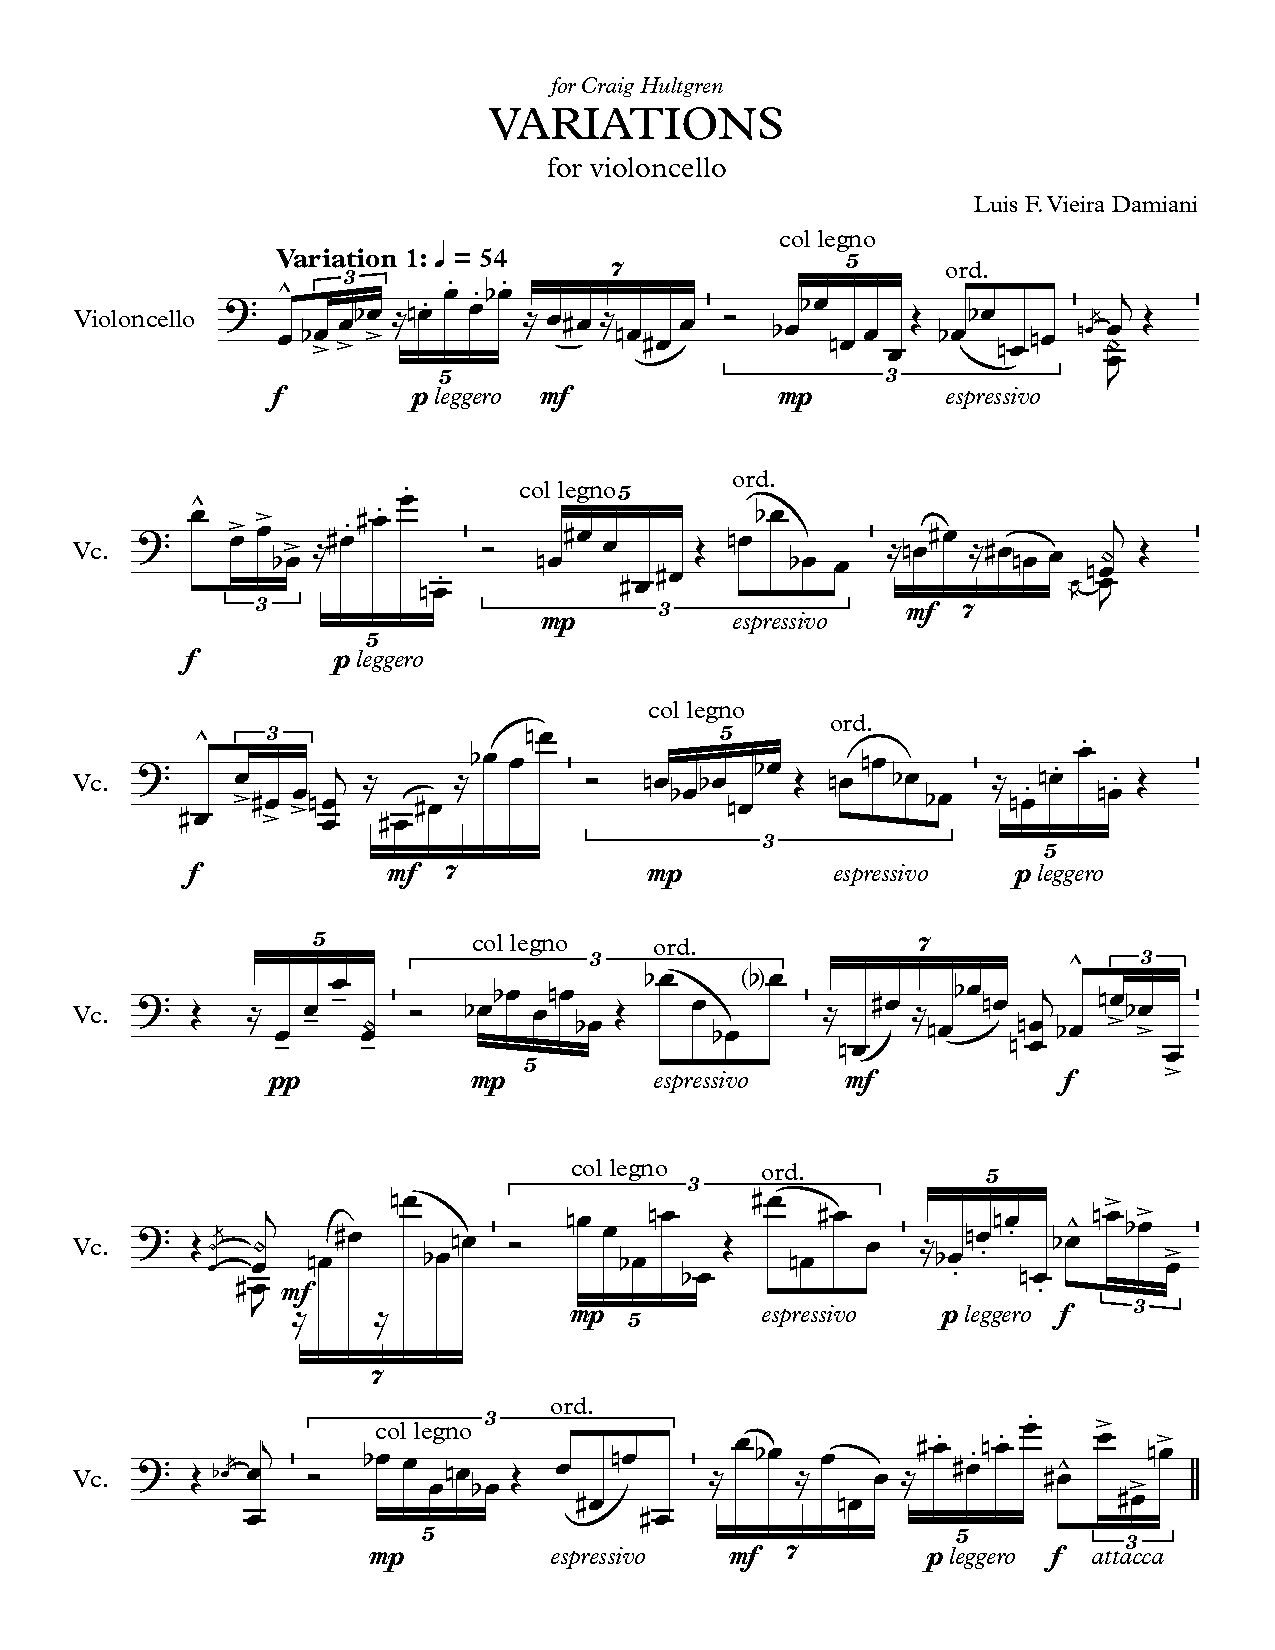
\includegraphics[width=6.5in]{figures/Variations_1.pdf}
\end{figure}

%--------------------------------------------------------------------------
\begin{figure}[htbp]
    \centering
	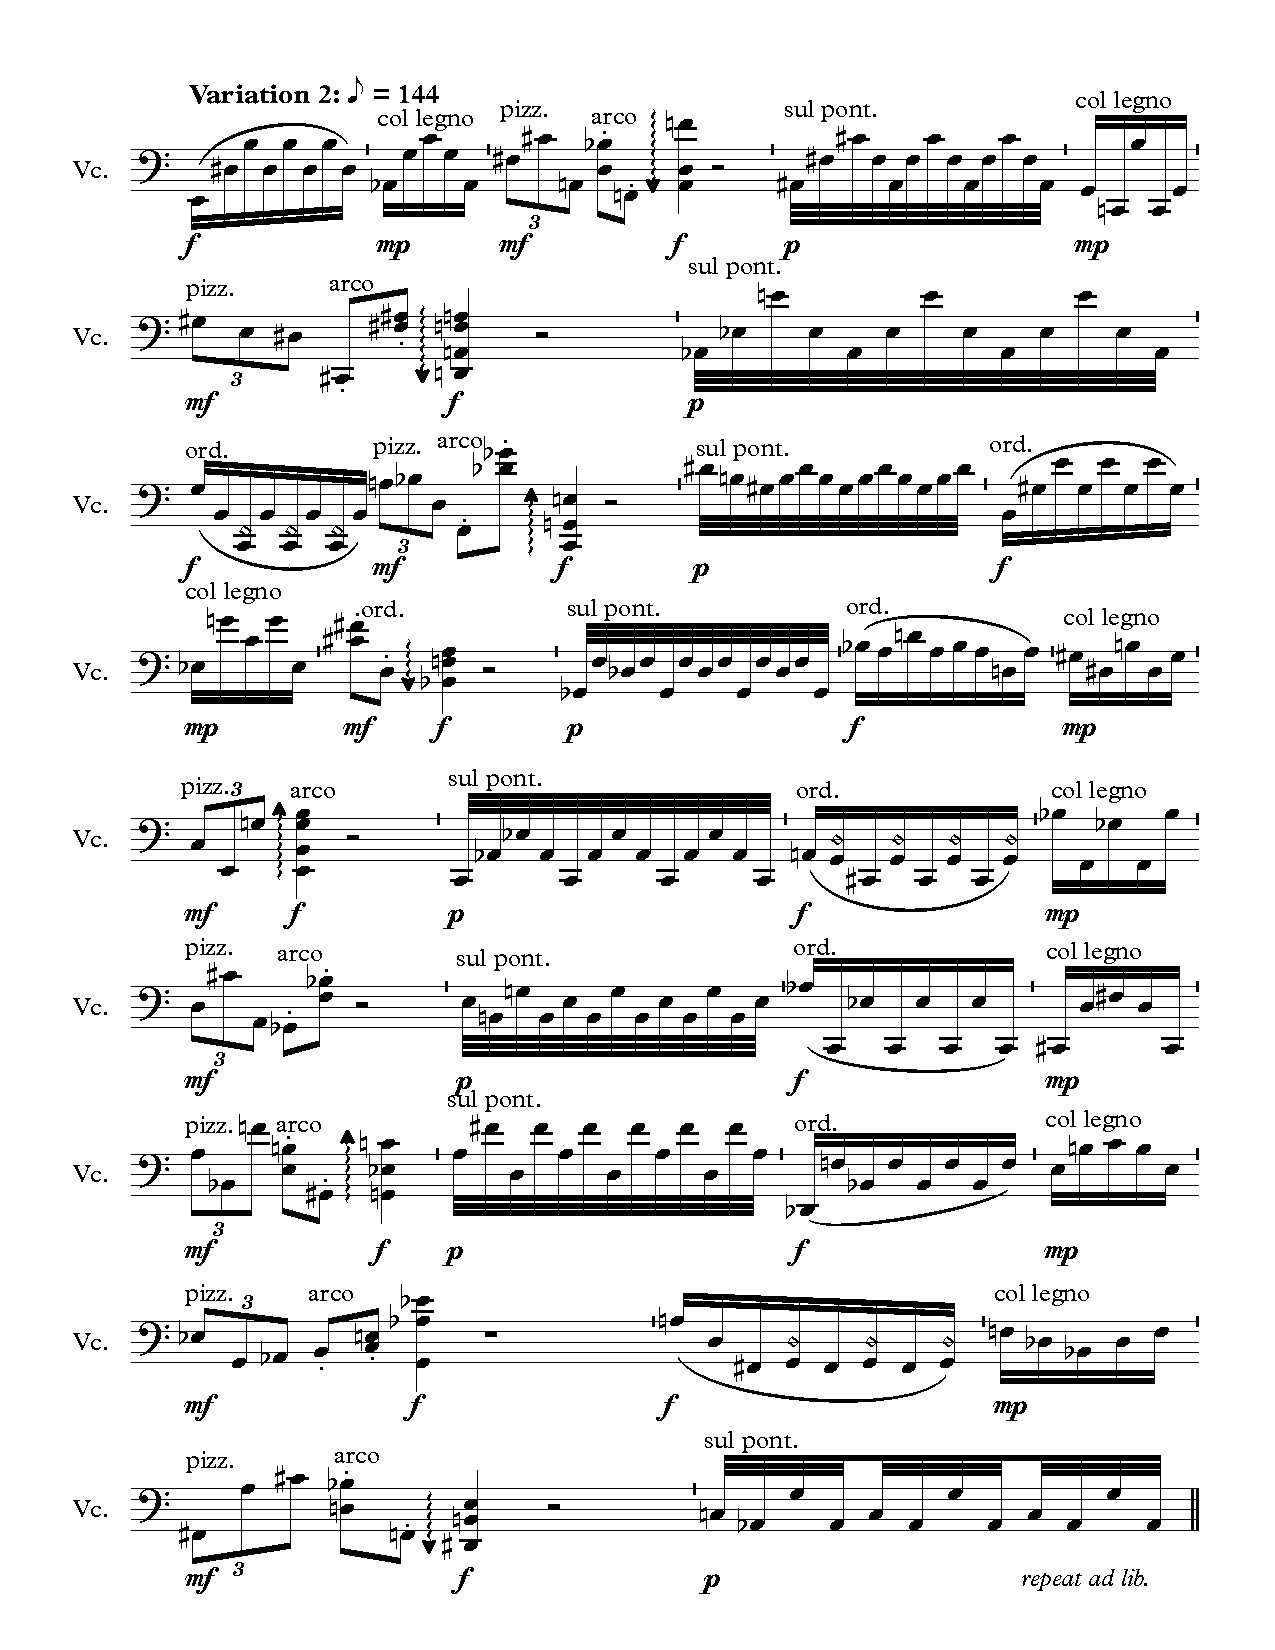
\includegraphics[width=6.5in]{figures/Variations_2.pdf}
\end{figure}

%--------------------------------------------------------------------------
\begin{figure}[htbp]
    \centering
	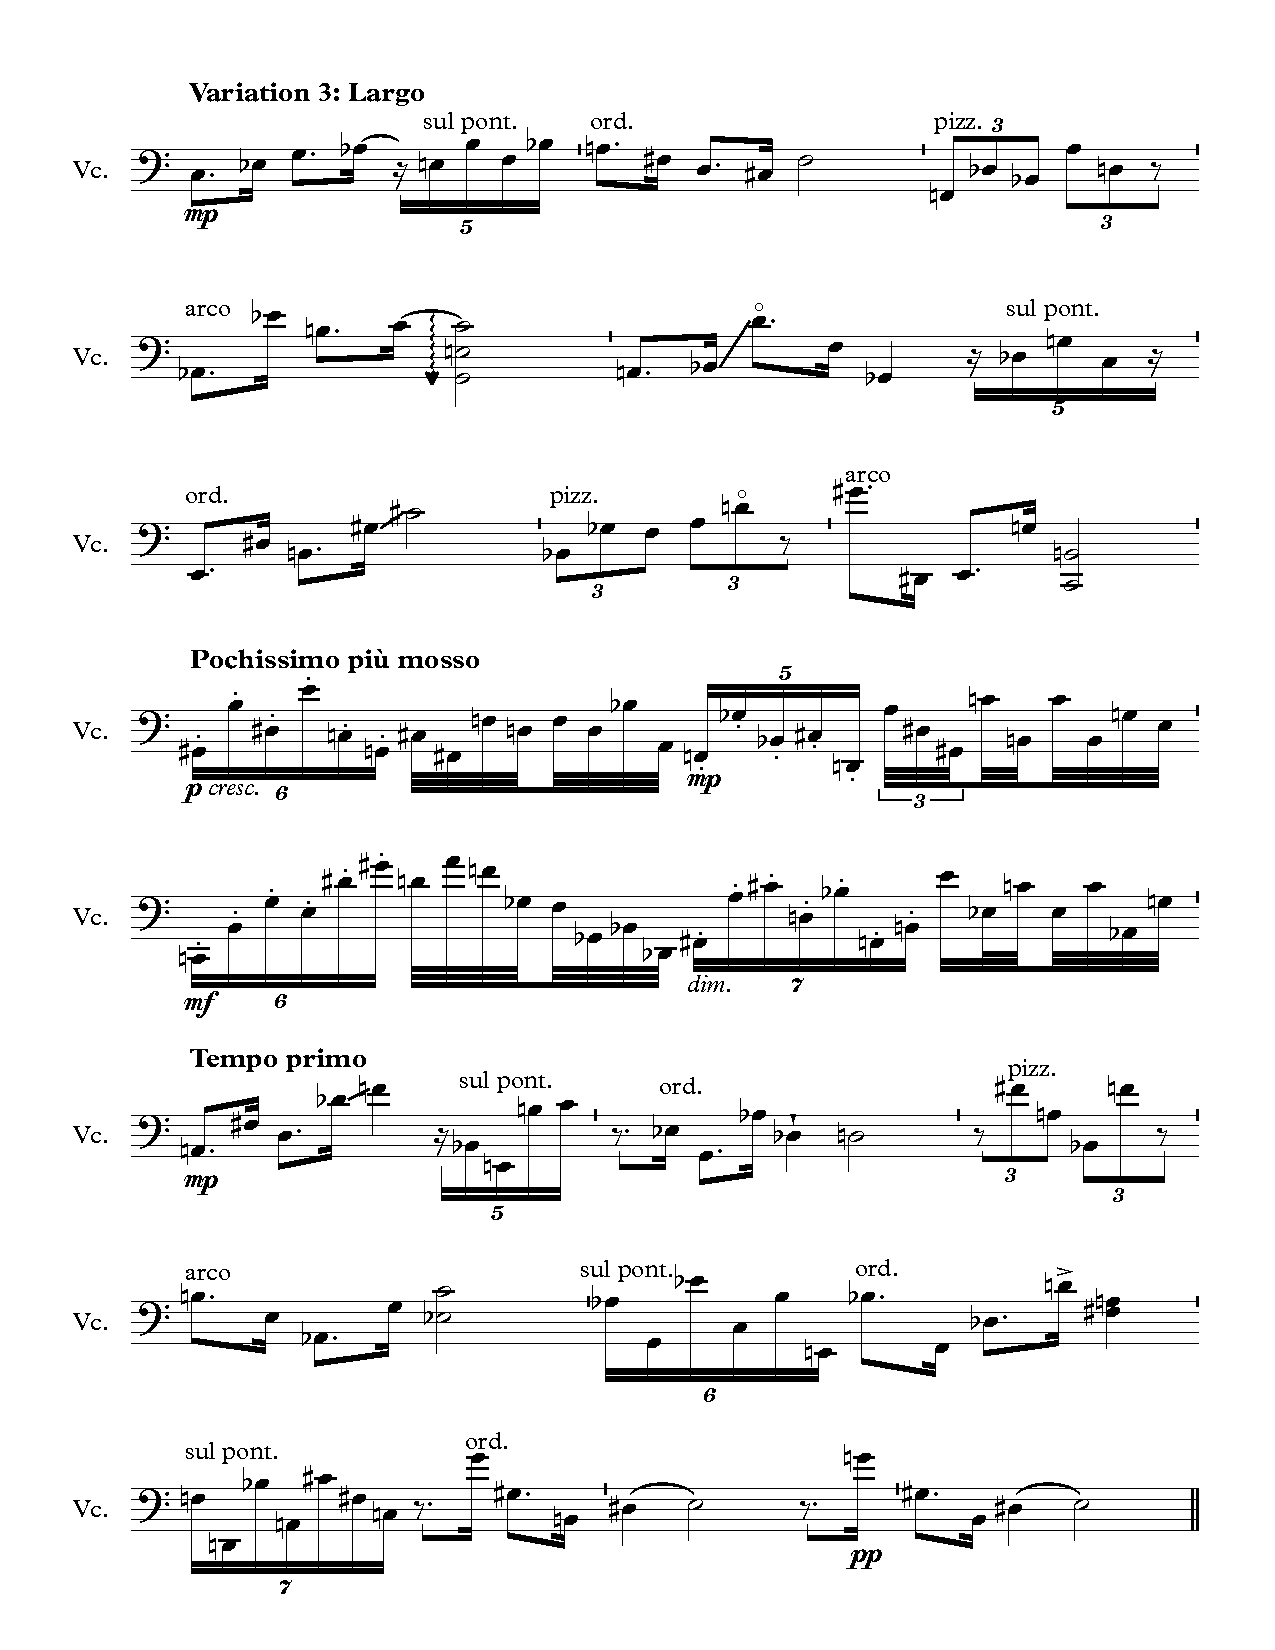
\includegraphics[width=6.5in]{figures/Variations_3.pdf}
\end{figure}

%--------------------------------------------------------------------------
\section{Program Notes}

%--------------------------------------------------------------------------
\emph{Variations for Violoncello} is a short piece in three movements written for Craig Hultgren, who premiered it at the University of Florida on October 21\textsuperscript{st} of 2013, shortly after it was written. The piece explores the serial technique of self-derivation, in which several layers of coherence occur simultaneously. A set of rhythmic motivic cells is imposed over the pitch structures. These cells are constantly rotated, and evolve at an independent pace from the self-deriving pitch structures, whose syntax of row transforms stay somewhat constant. This procedure ultimately defines the impetus of the piece, where the quasi-kaleidoscopic nature of the pitch domain is driven by the ever free-spirited rhythmic motives.

%--------------------------------------------------------------------------
\chapter{Stabat Mater}

%--------------------------------------------------------------------------
\begin{figure}[h!]
    \centering
	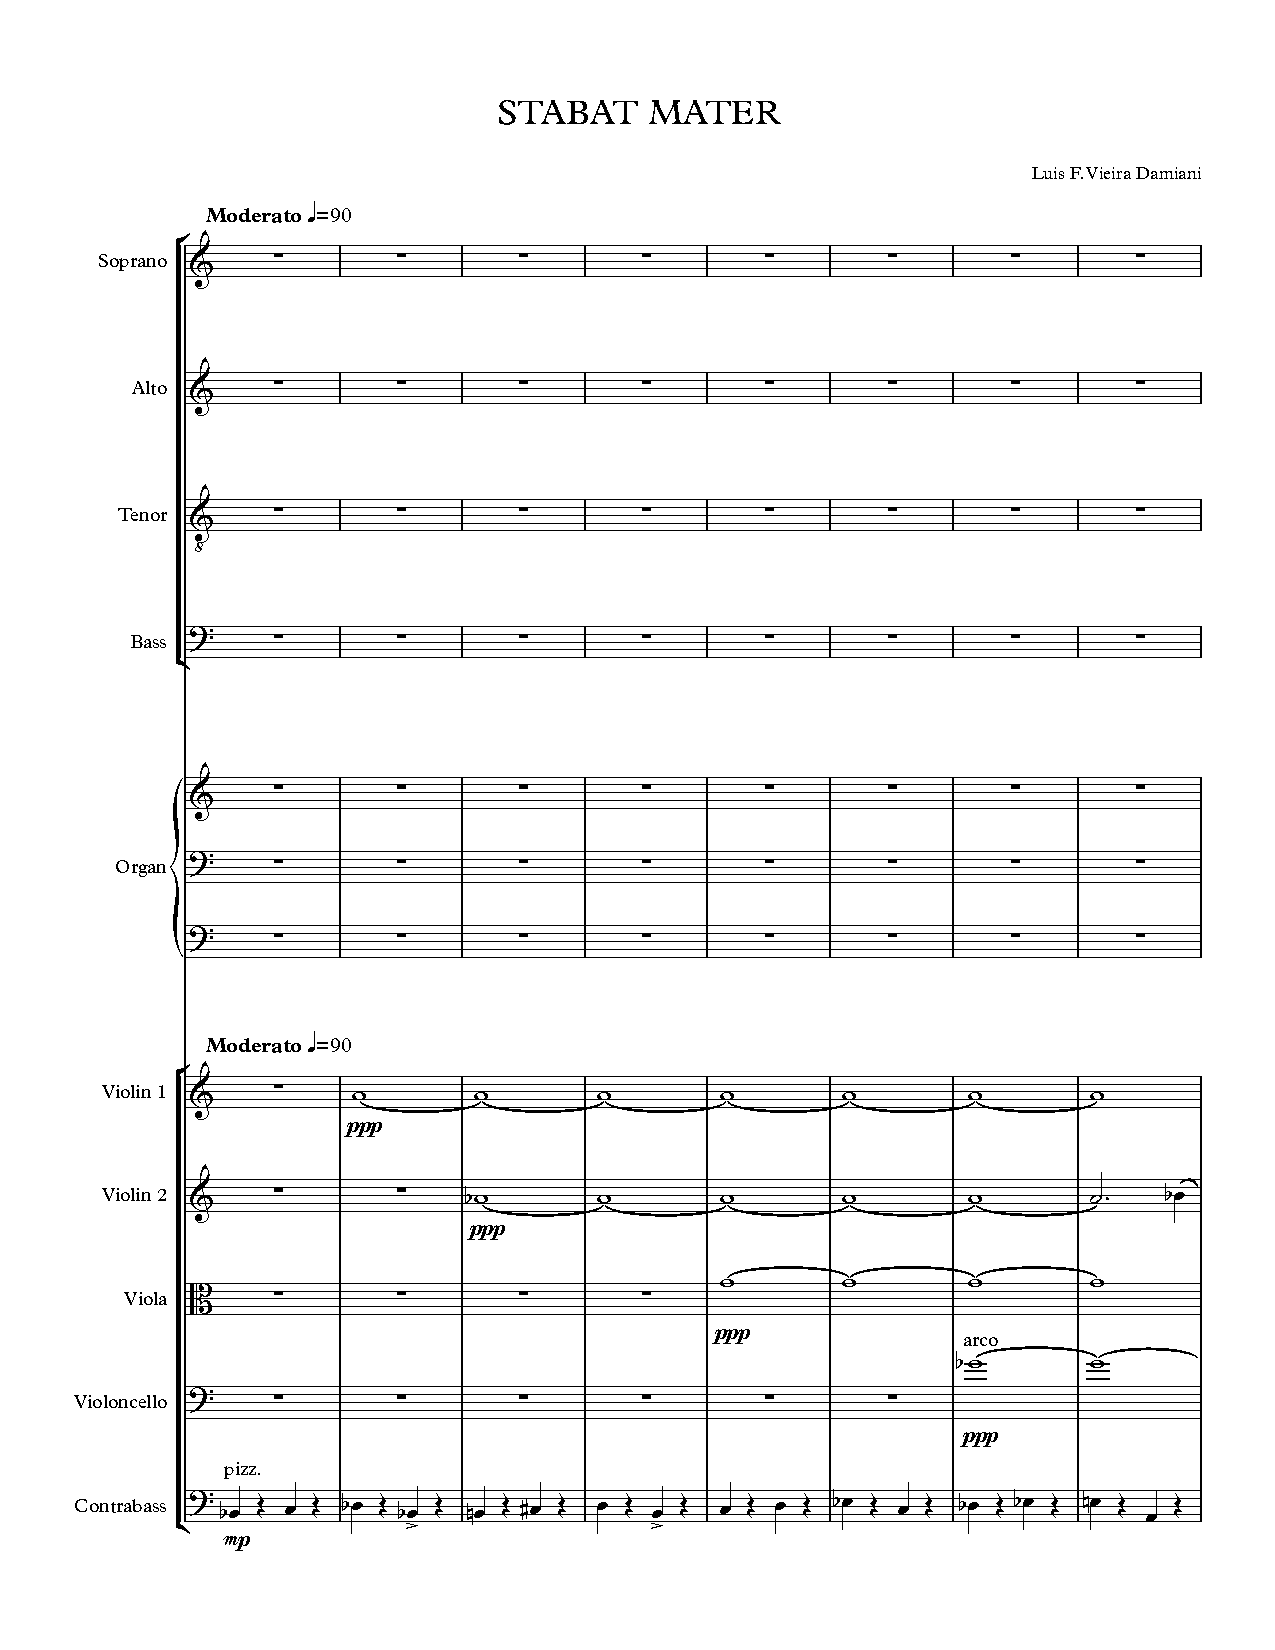
\includegraphics[width=6.5in]{figures/Stabat_Mater_1.pdf}
\end{figure}

%--------------------------------------------------------------------------
\begin{figure}[htbp]
    \centering
	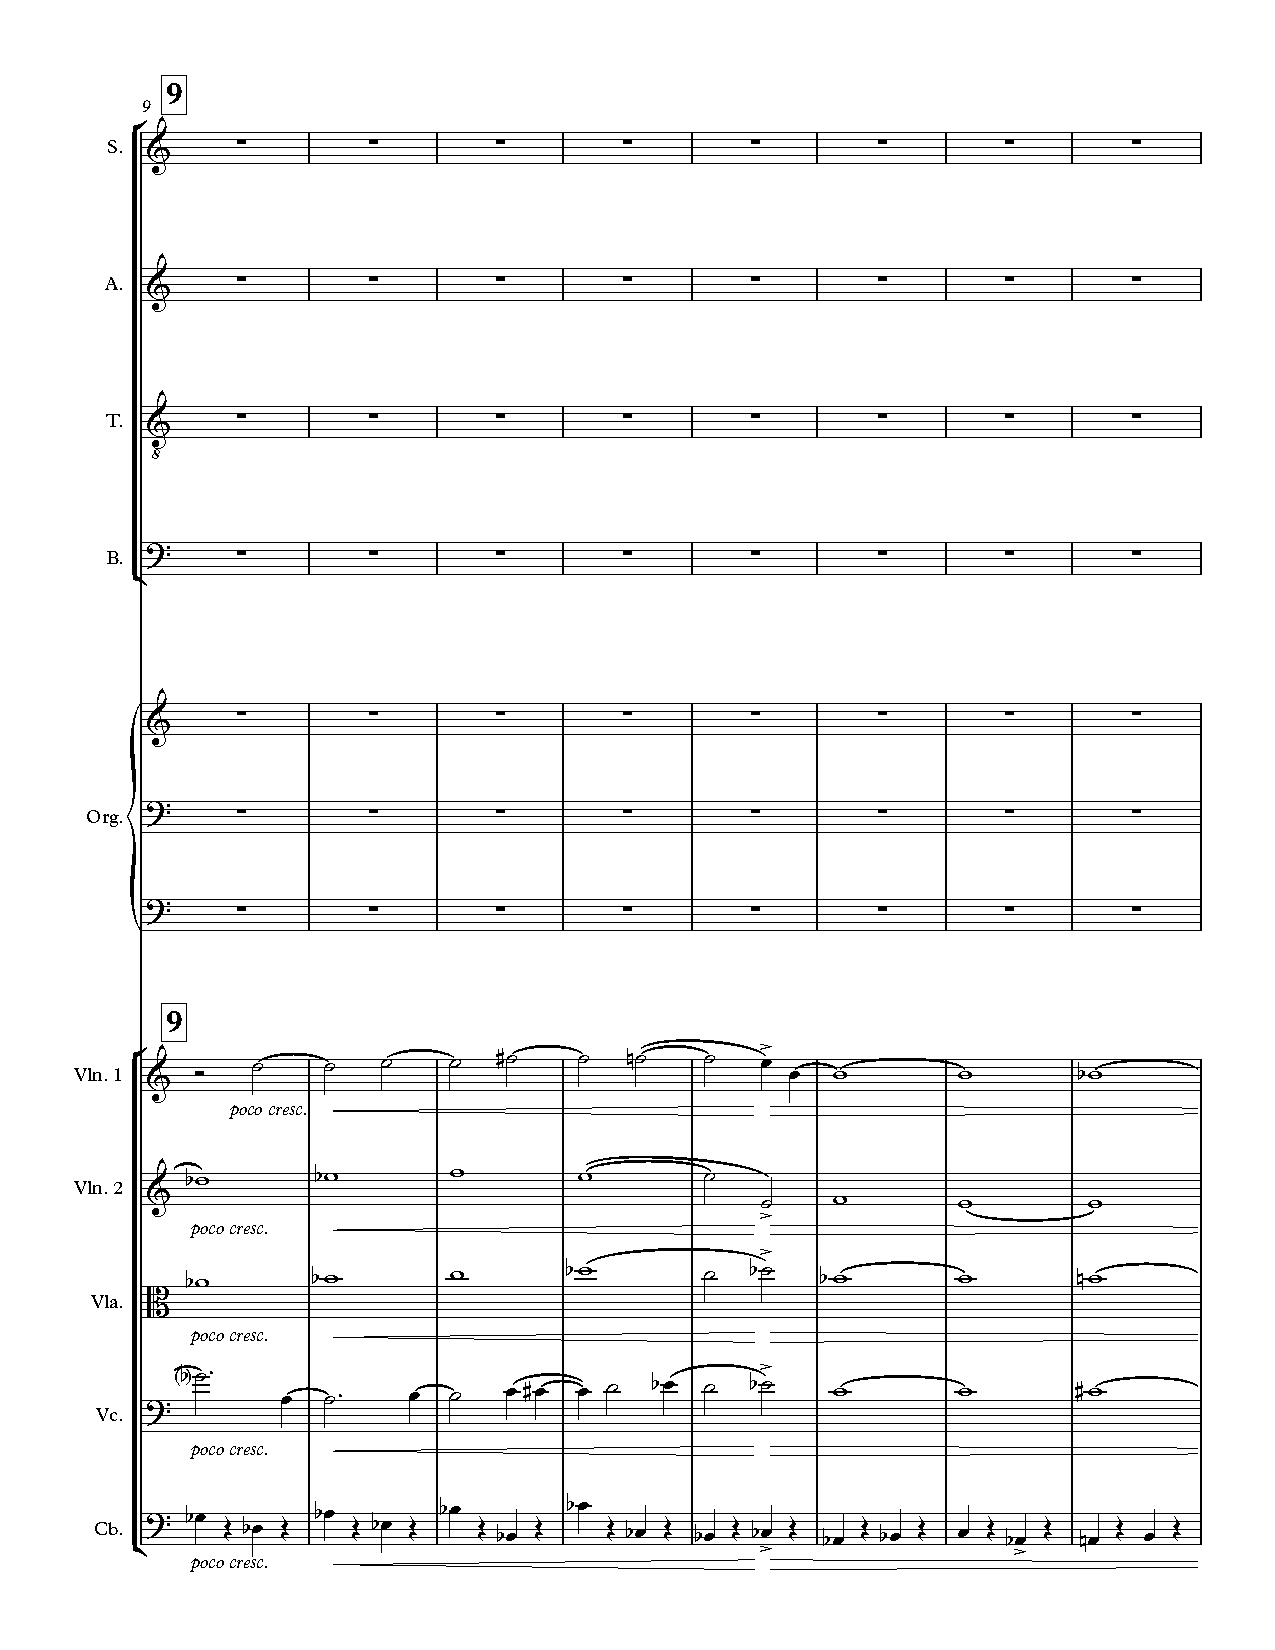
\includegraphics[width=6.5in]{figures/Stabat_Mater_2.pdf}
\end{figure}

%--------------------------------------------------------------------------
\begin{figure}[htbp]
    \centering
	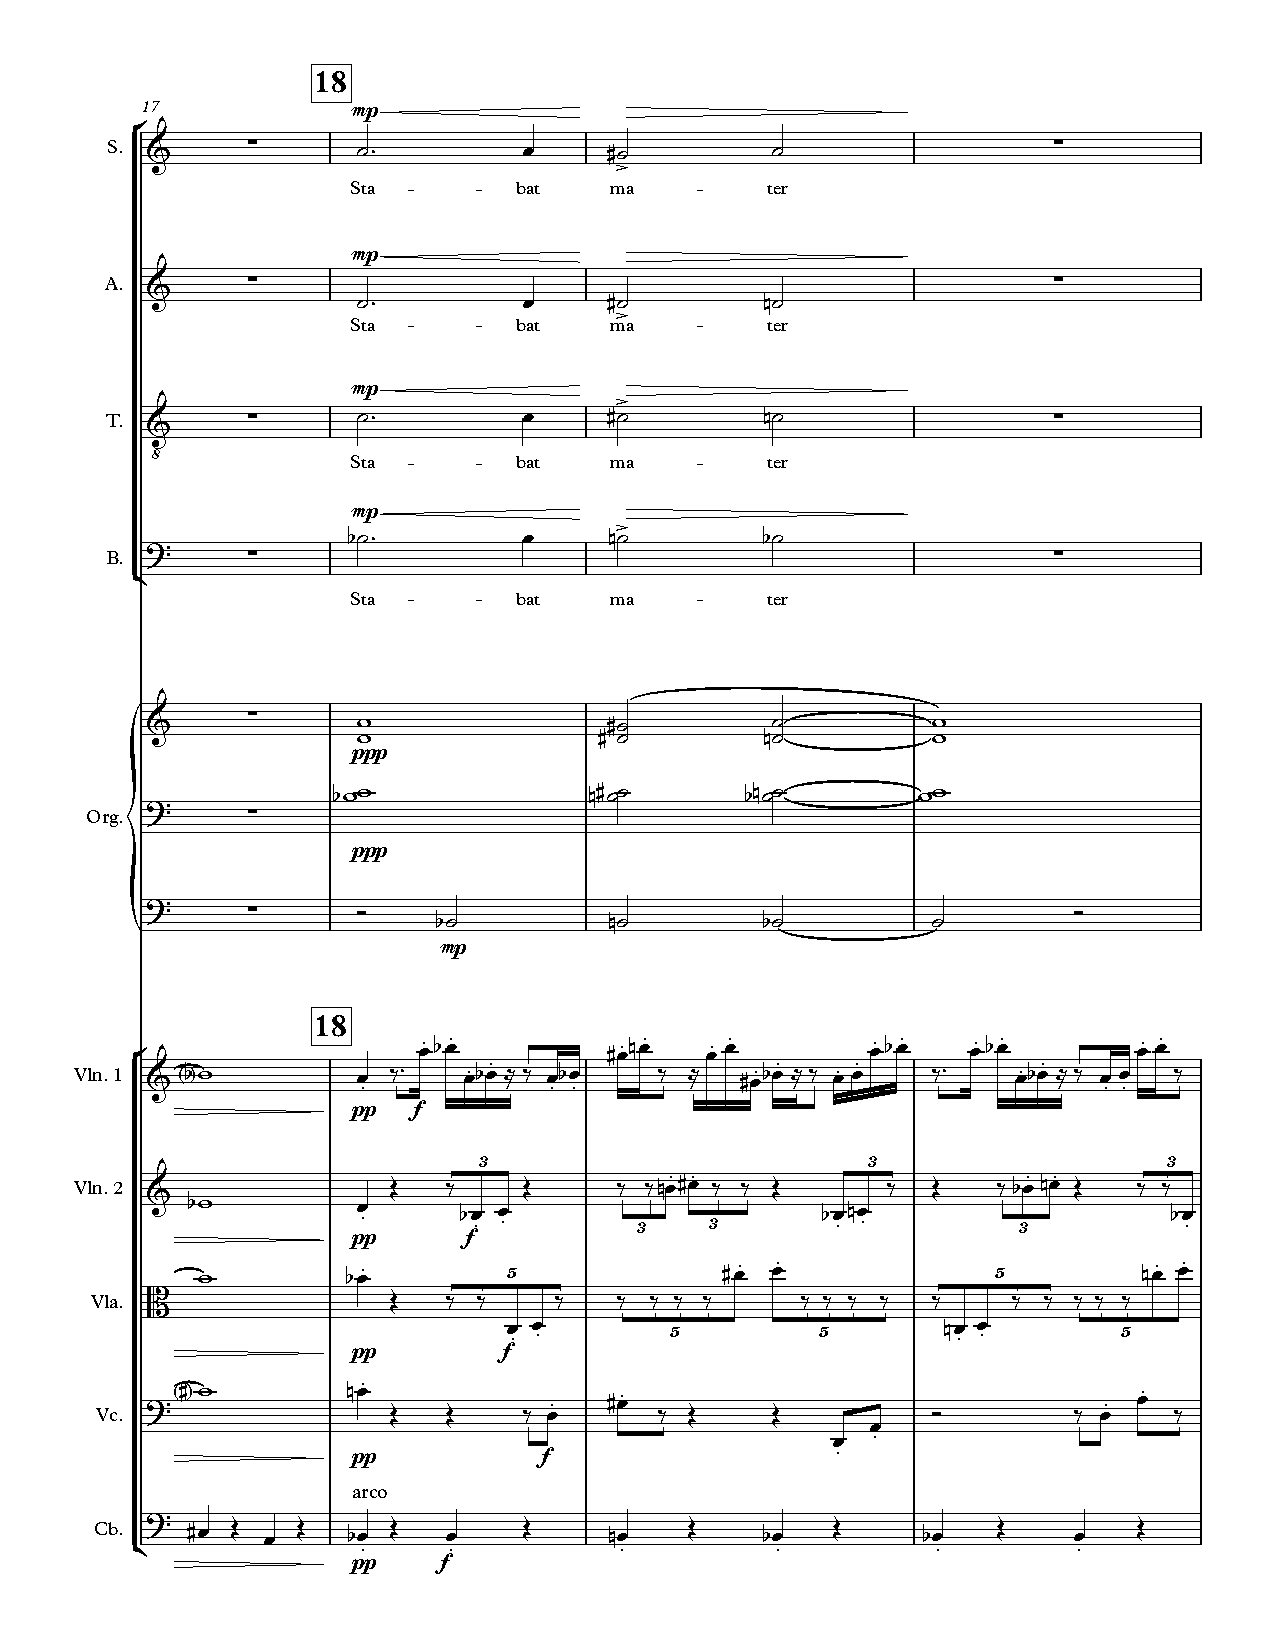
\includegraphics[width=6.5in]{figures/Stabat_Mater_3.pdf}
\end{figure}

%--------------------------------------------------------------------------
\begin{figure}[htbp]
    \centering
	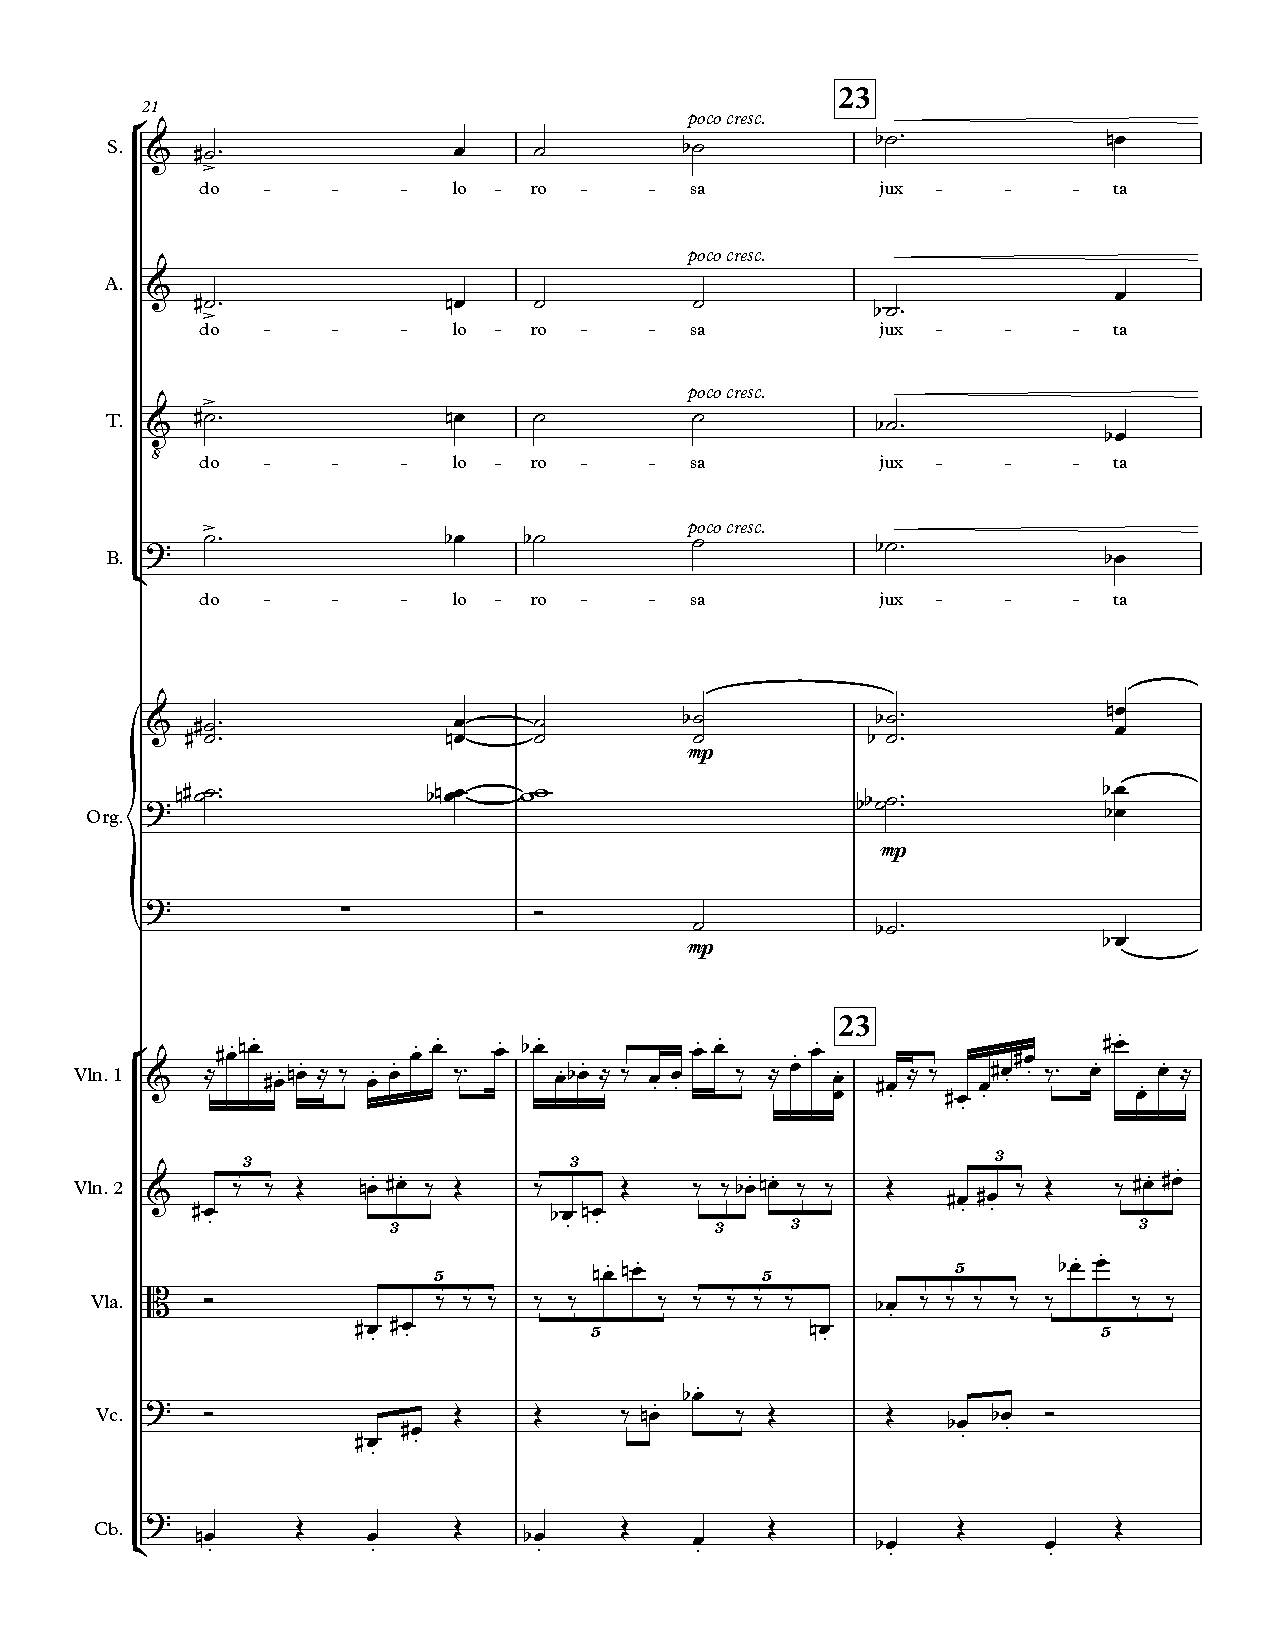
\includegraphics[width=6.5in]{figures/Stabat_Mater_4.pdf}
\end{figure}

%--------------------------------------------------------------------------
\begin{figure}[htbp]
    \centering
	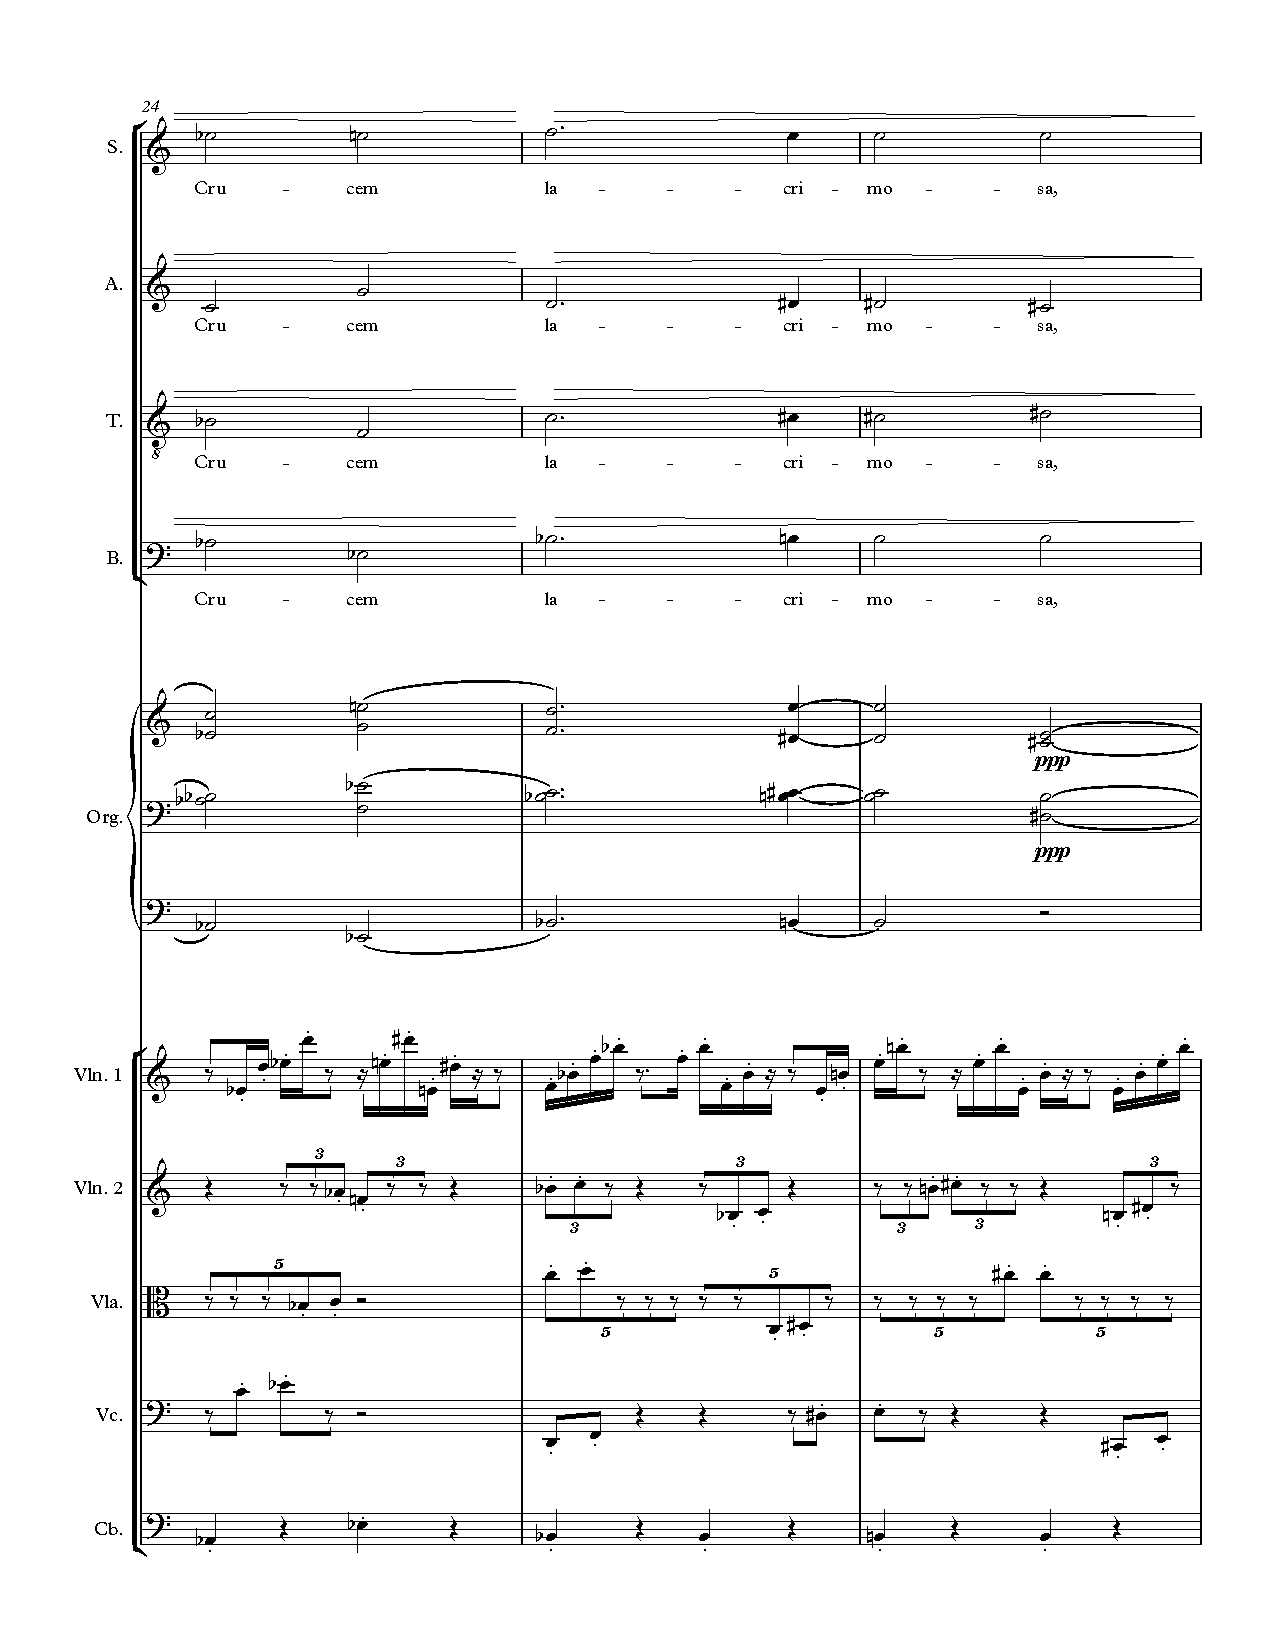
\includegraphics[width=6.5in]{figures/Stabat_Mater_5.pdf}
\end{figure}

%--------------------------------------------------------------------------
\begin{figure}[htbp]
    \centering
	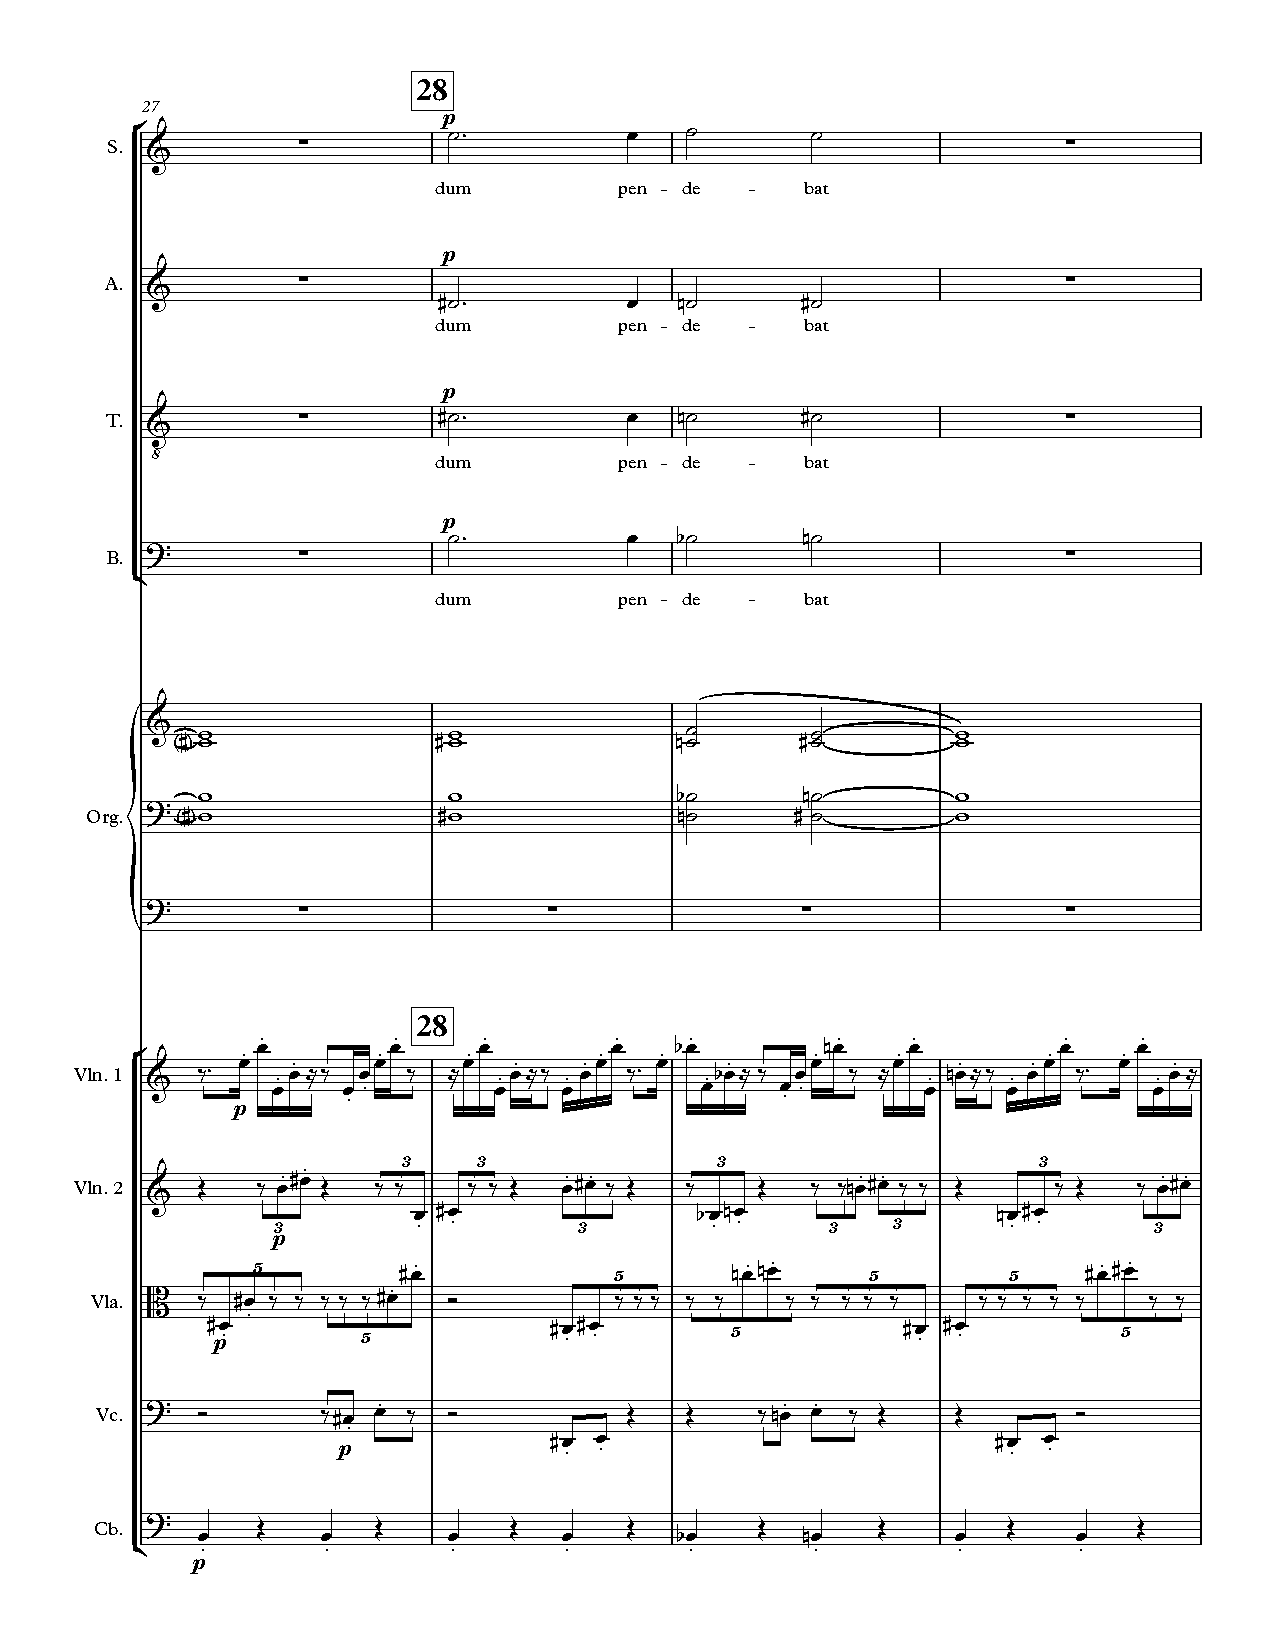
\includegraphics[width=6.5in]{figures/Stabat_Mater_6.pdf}
\end{figure}

%--------------------------------------------------------------------------
\begin{figure}[htbp]
    \centering
	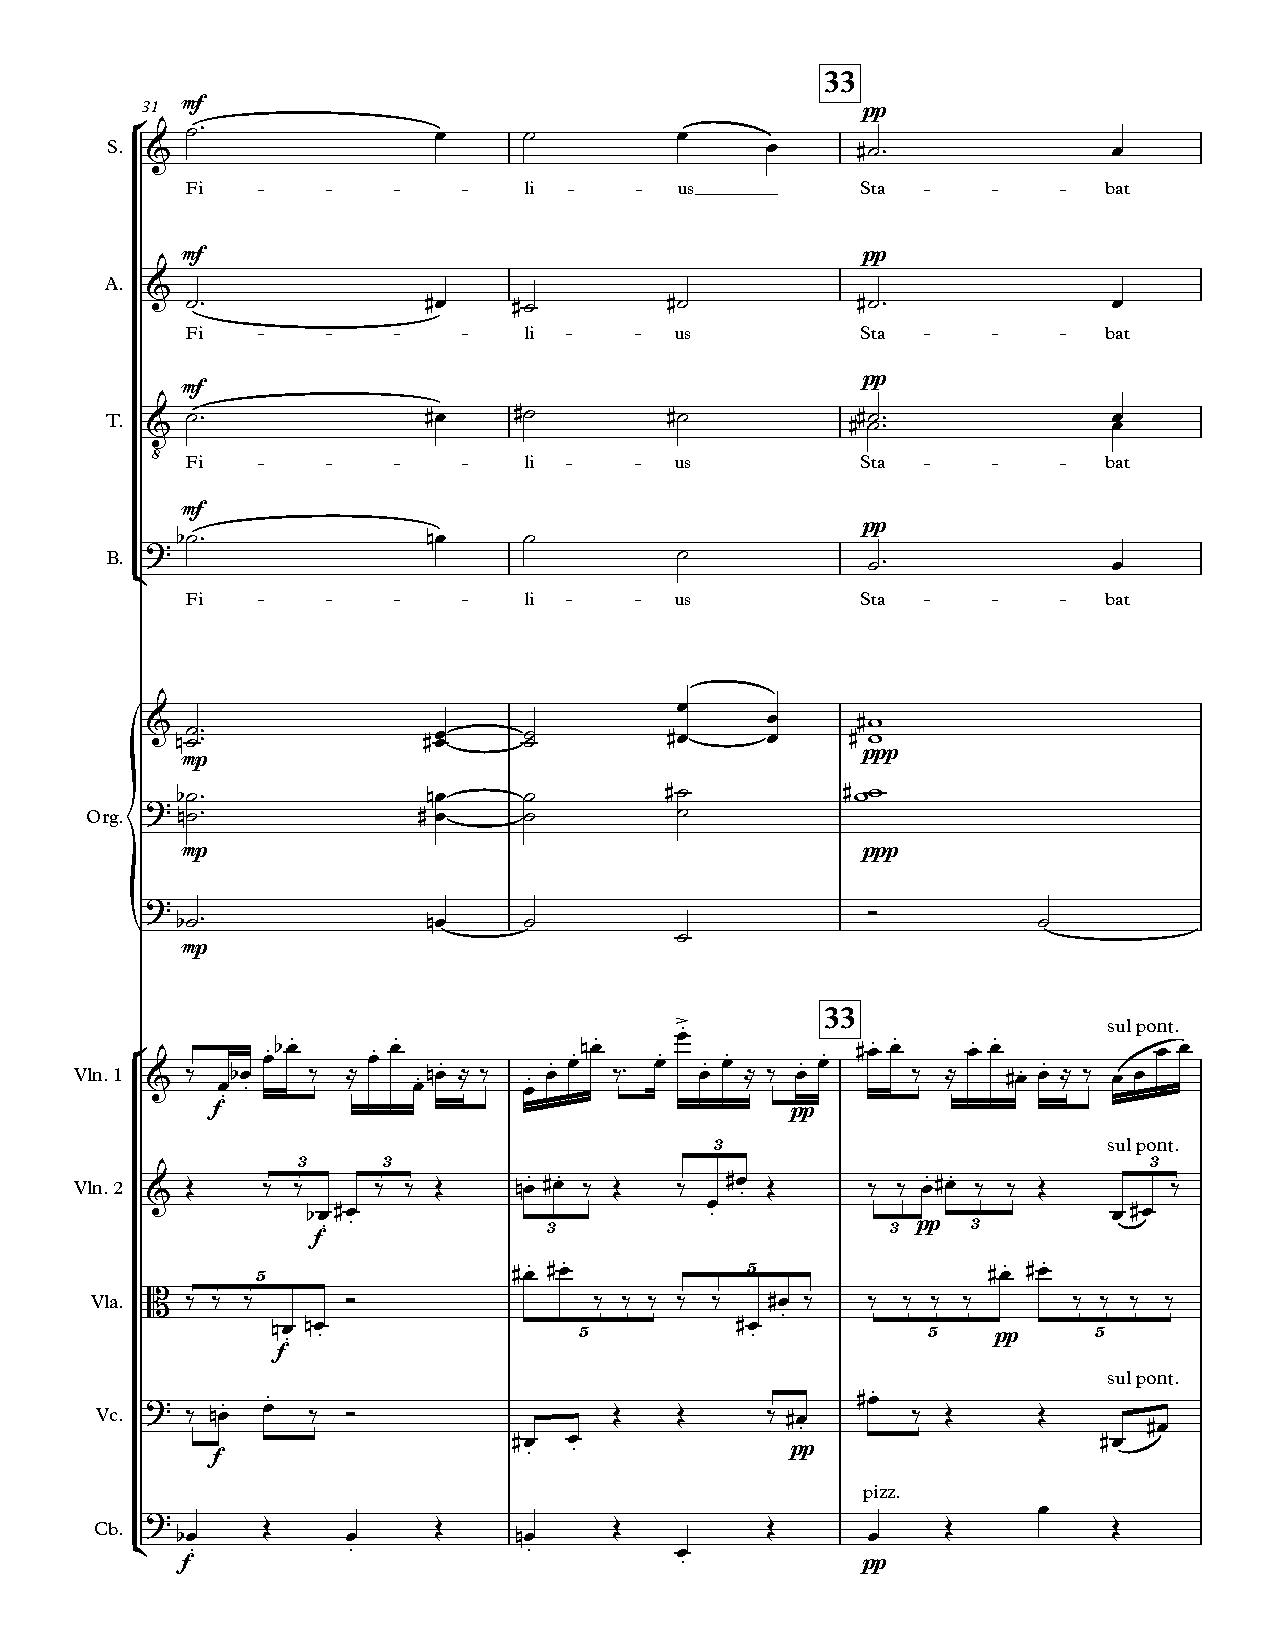
\includegraphics[width=6.5in]{figures/Stabat_Mater_7.pdf}
\end{figure}

%--------------------------------------------------------------------------
\begin{figure}[htbp]
    \centering
	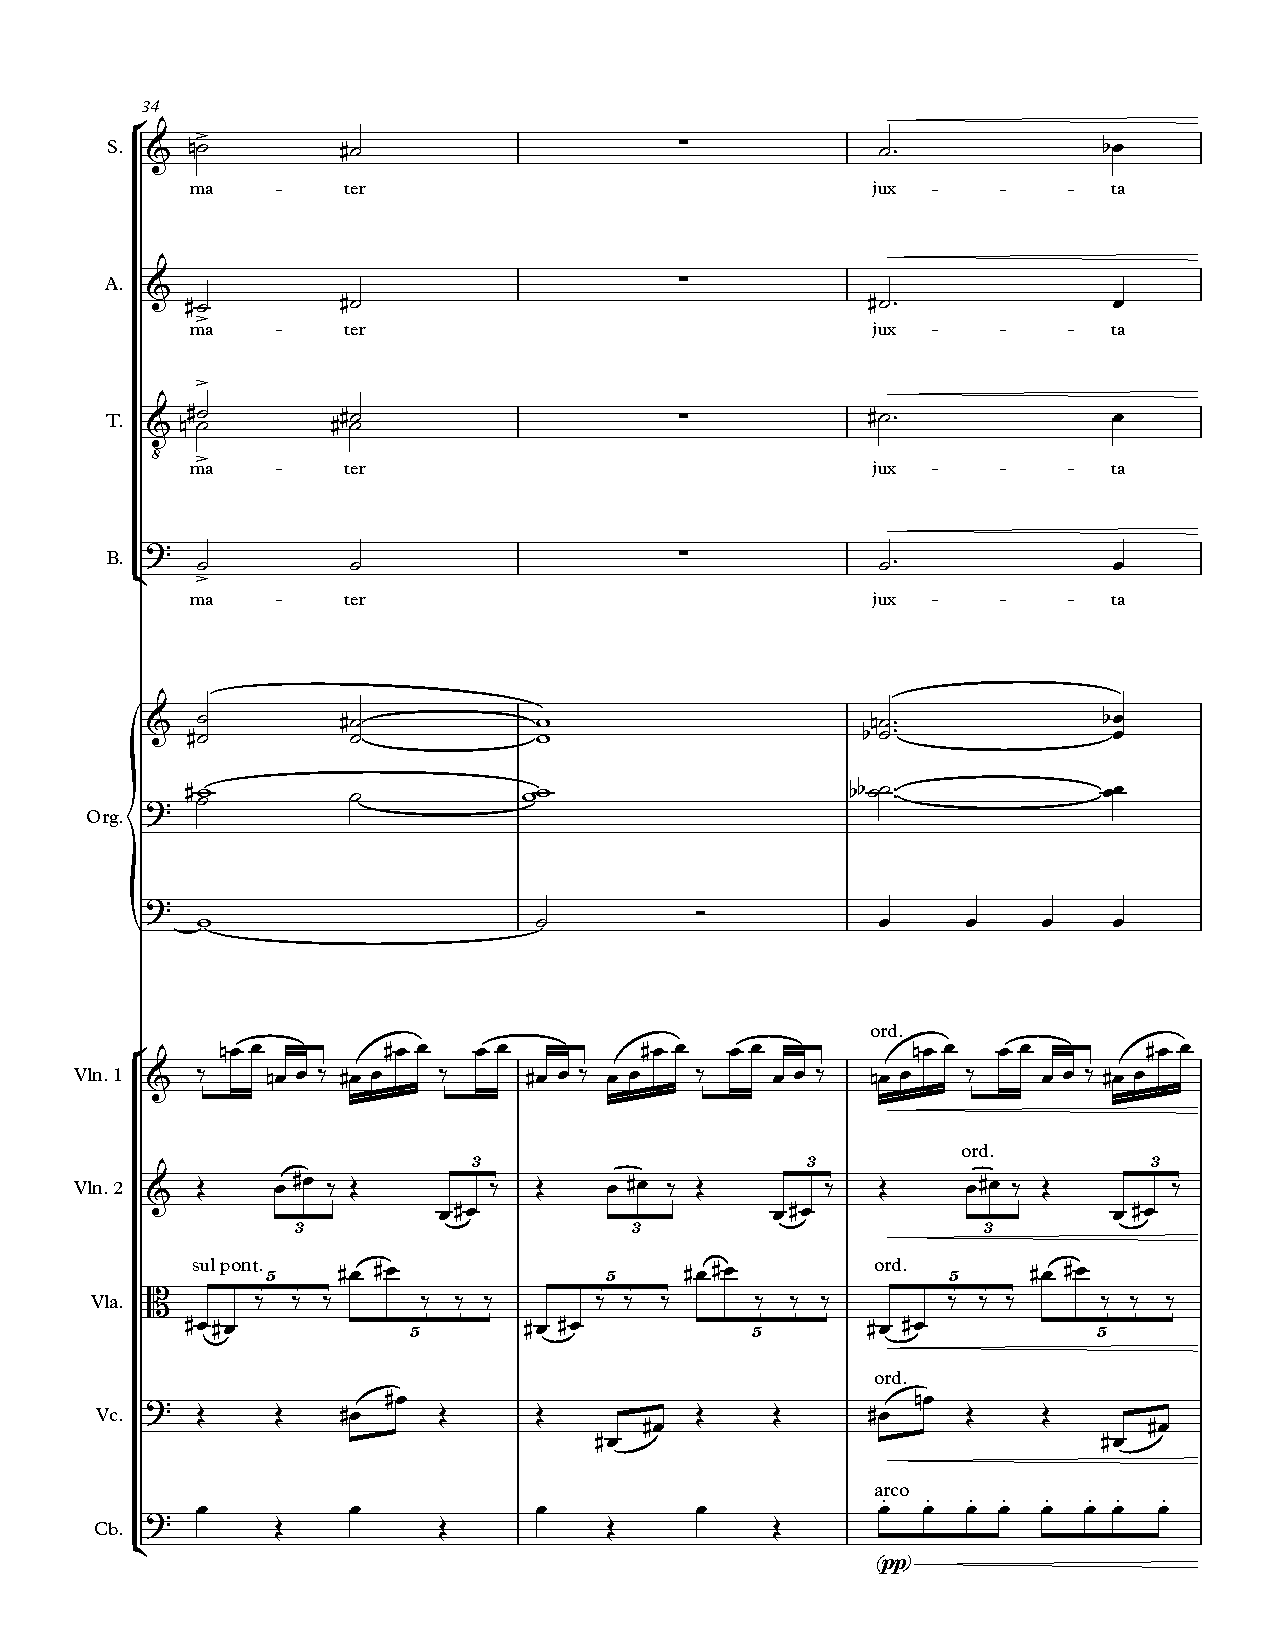
\includegraphics[width=6.5in]{figures/Stabat_Mater_8.pdf}
\end{figure}

%--------------------------------------------------------------------------
\begin{figure}[htbp]
    \centering
	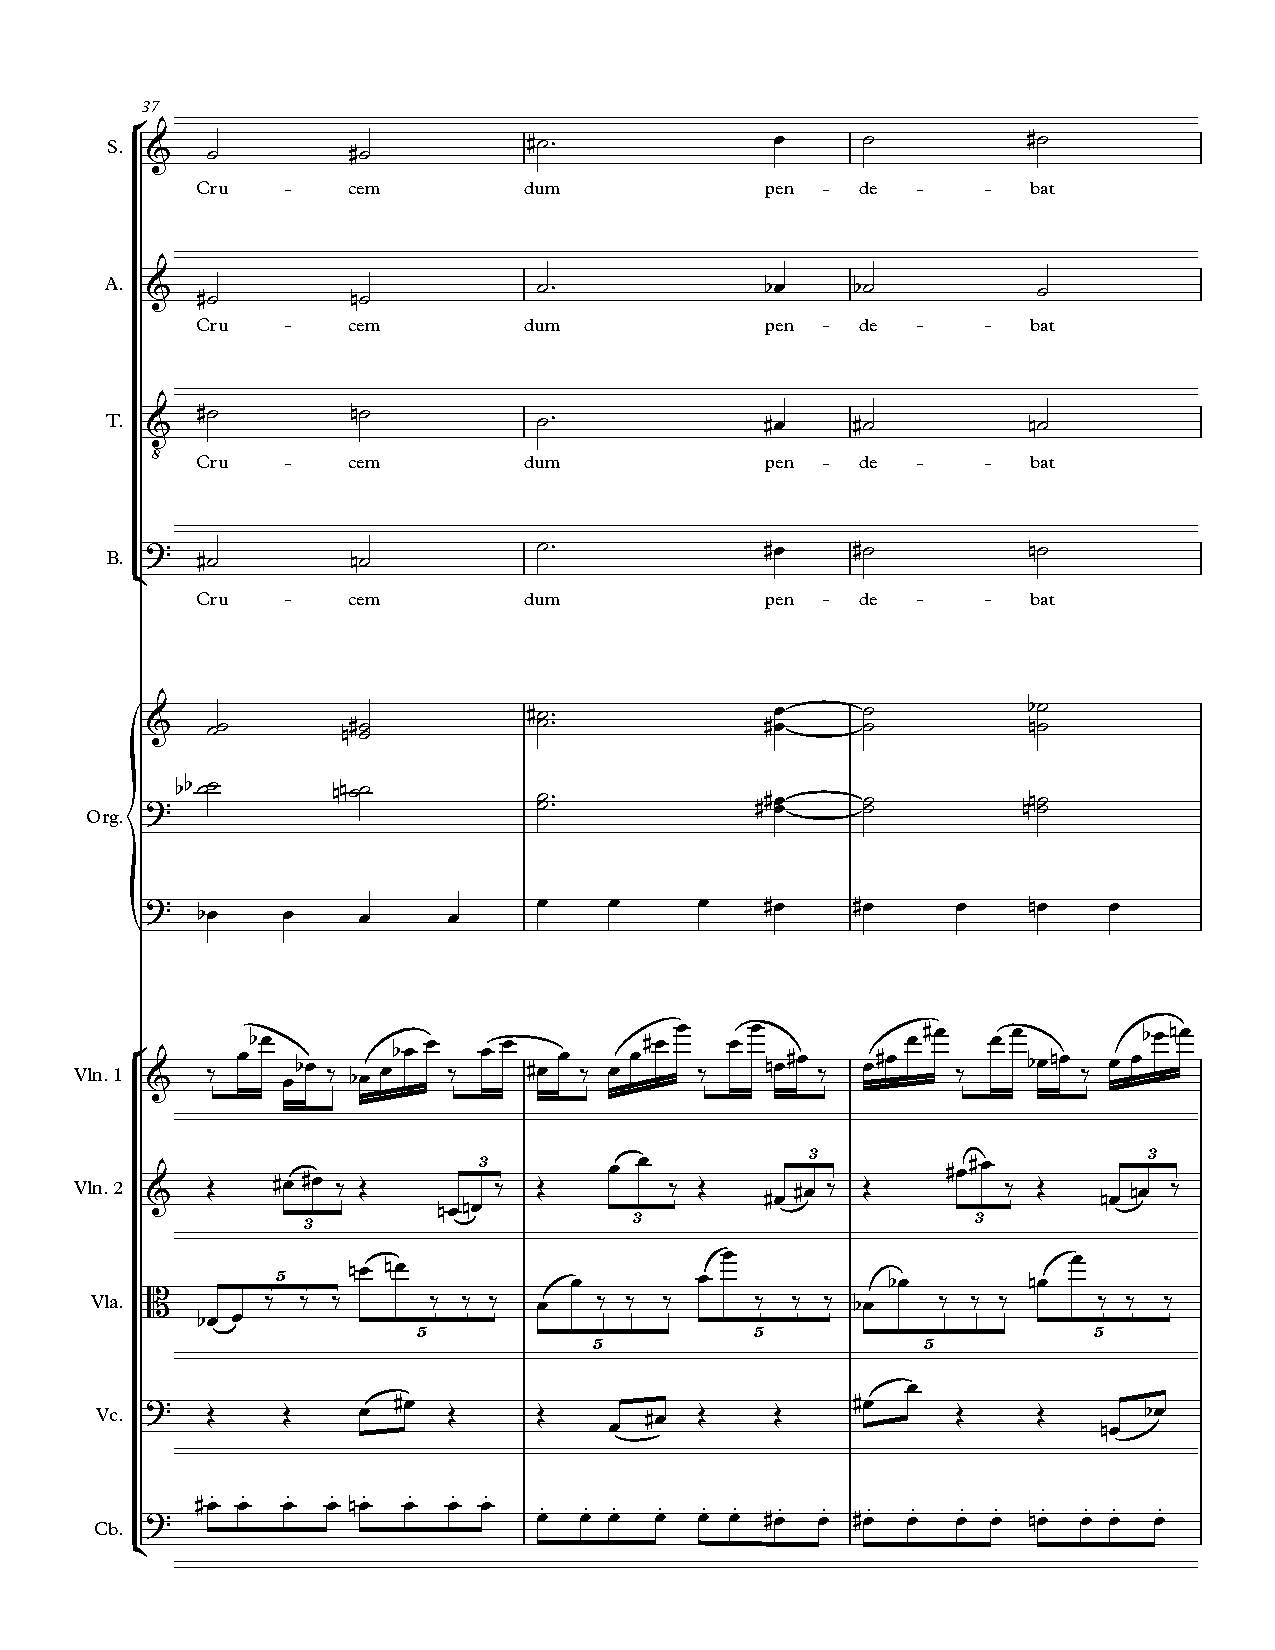
\includegraphics[width=6.5in]{figures/Stabat_Mater_9.pdf}
\end{figure}

%--------------------------------------------------------------------------
\begin{figure}[htbp]
    \centering
	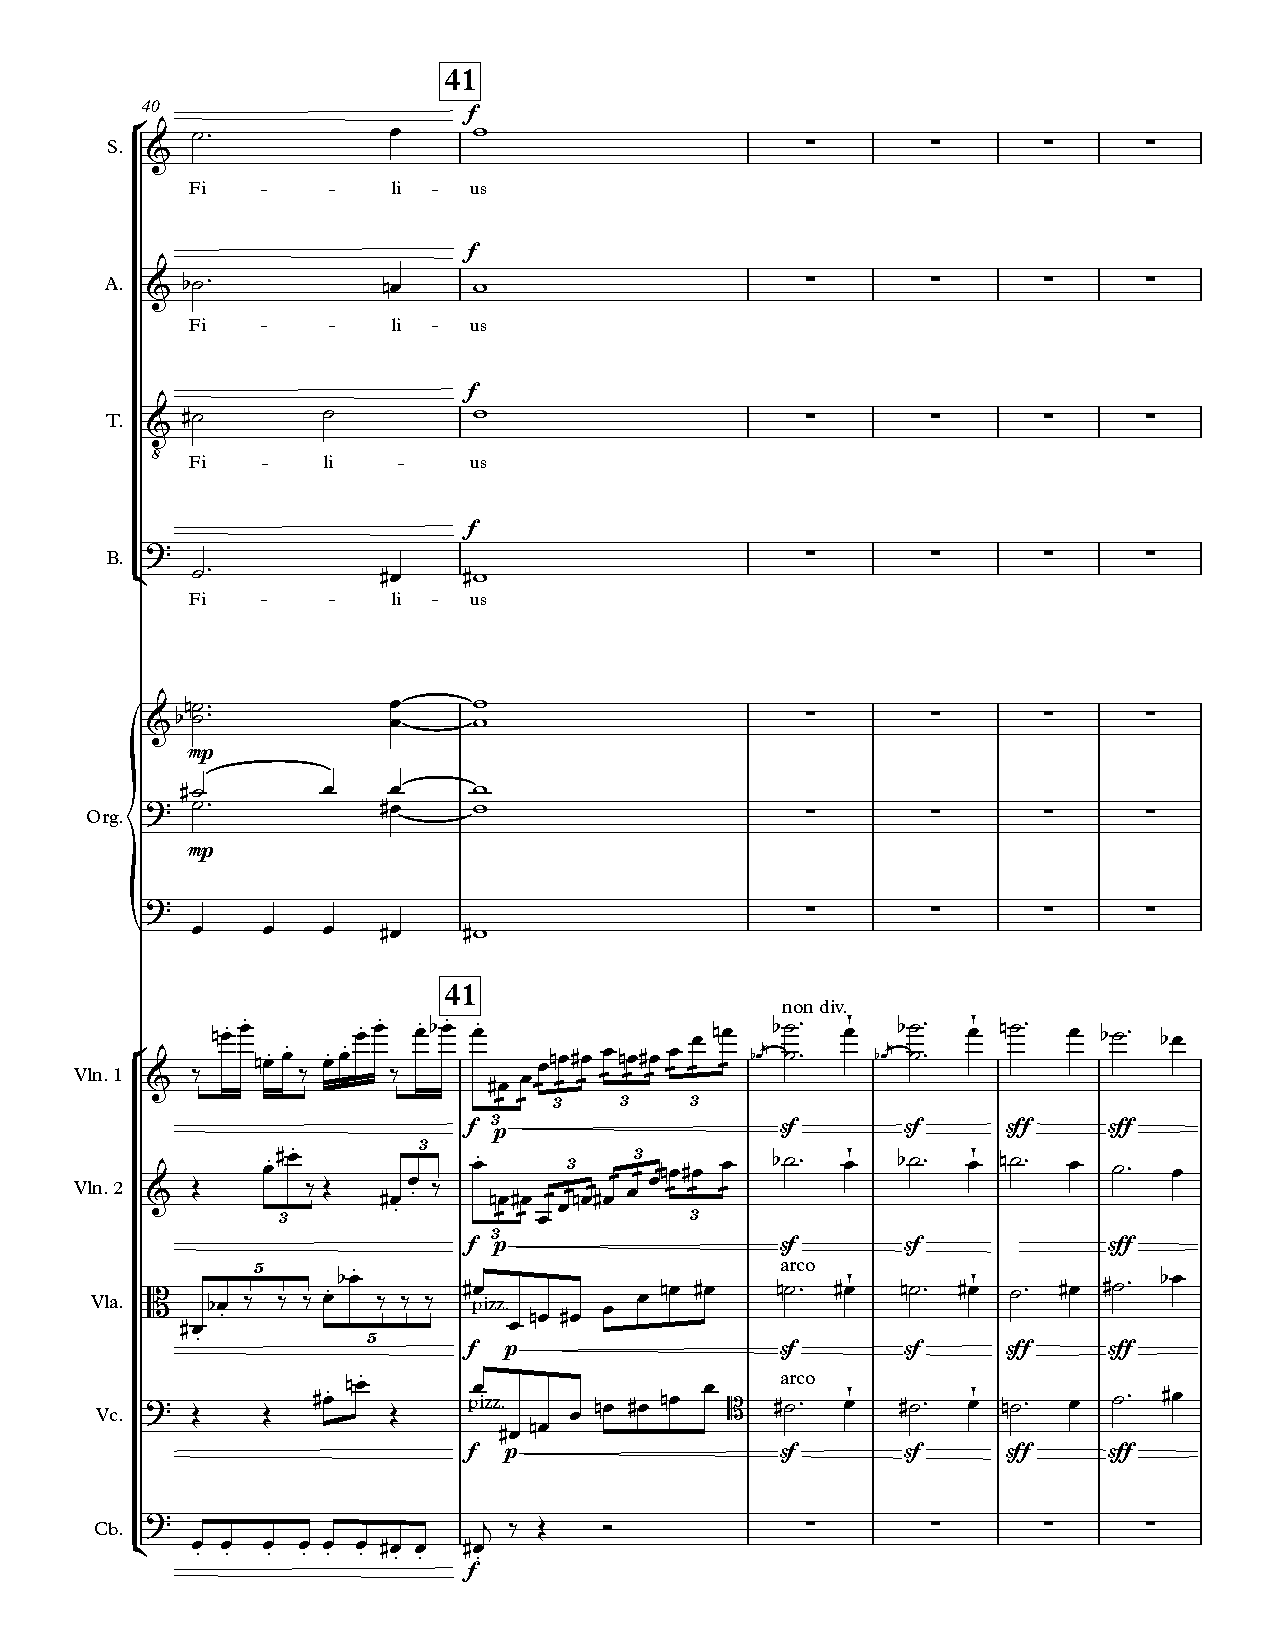
\includegraphics[width=6.5in]{figures/Stabat_Mater_10.pdf}
\end{figure}

%--------------------------------------------------------------------------
\begin{figure}[htbp]
    \centering
	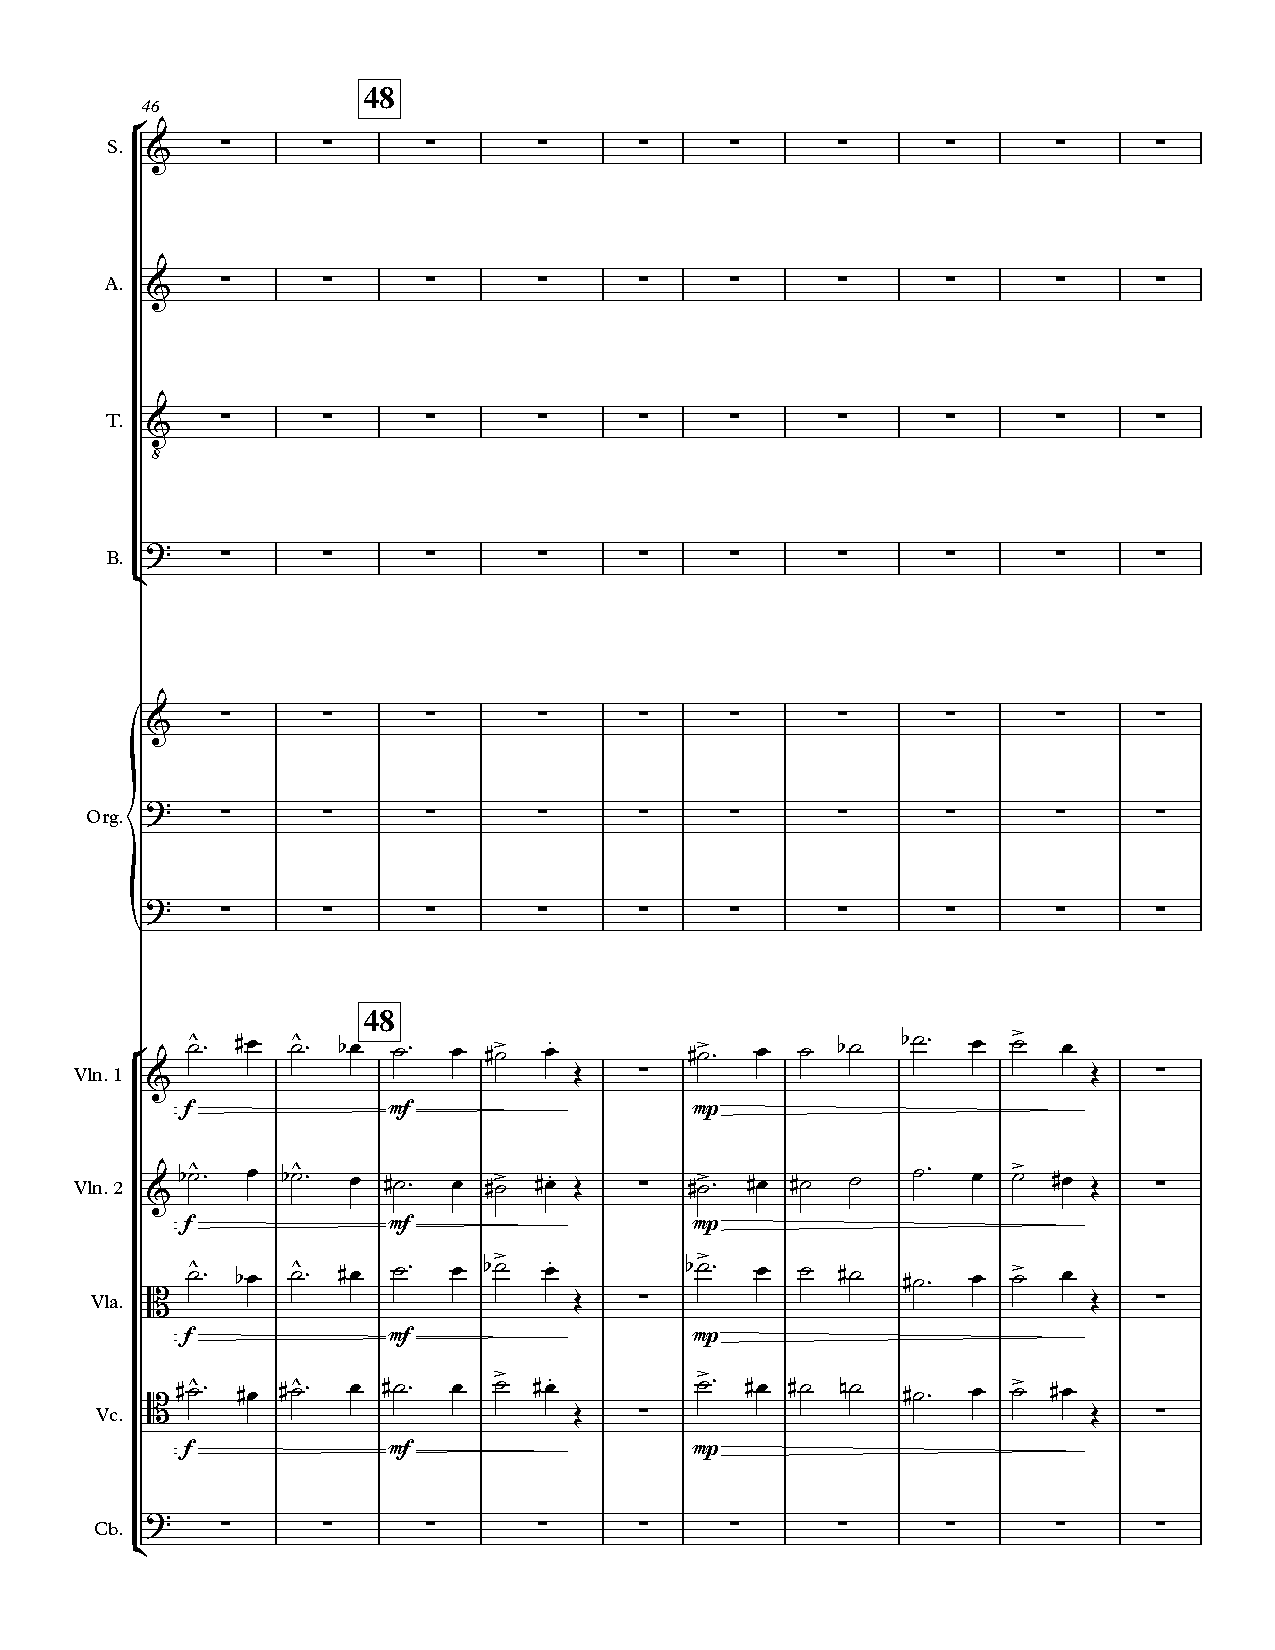
\includegraphics[width=6.5in]{figures/Stabat_Mater_11.pdf}
\end{figure}

%--------------------------------------------------------------------------
\begin{figure}[htbp]
    \centering
	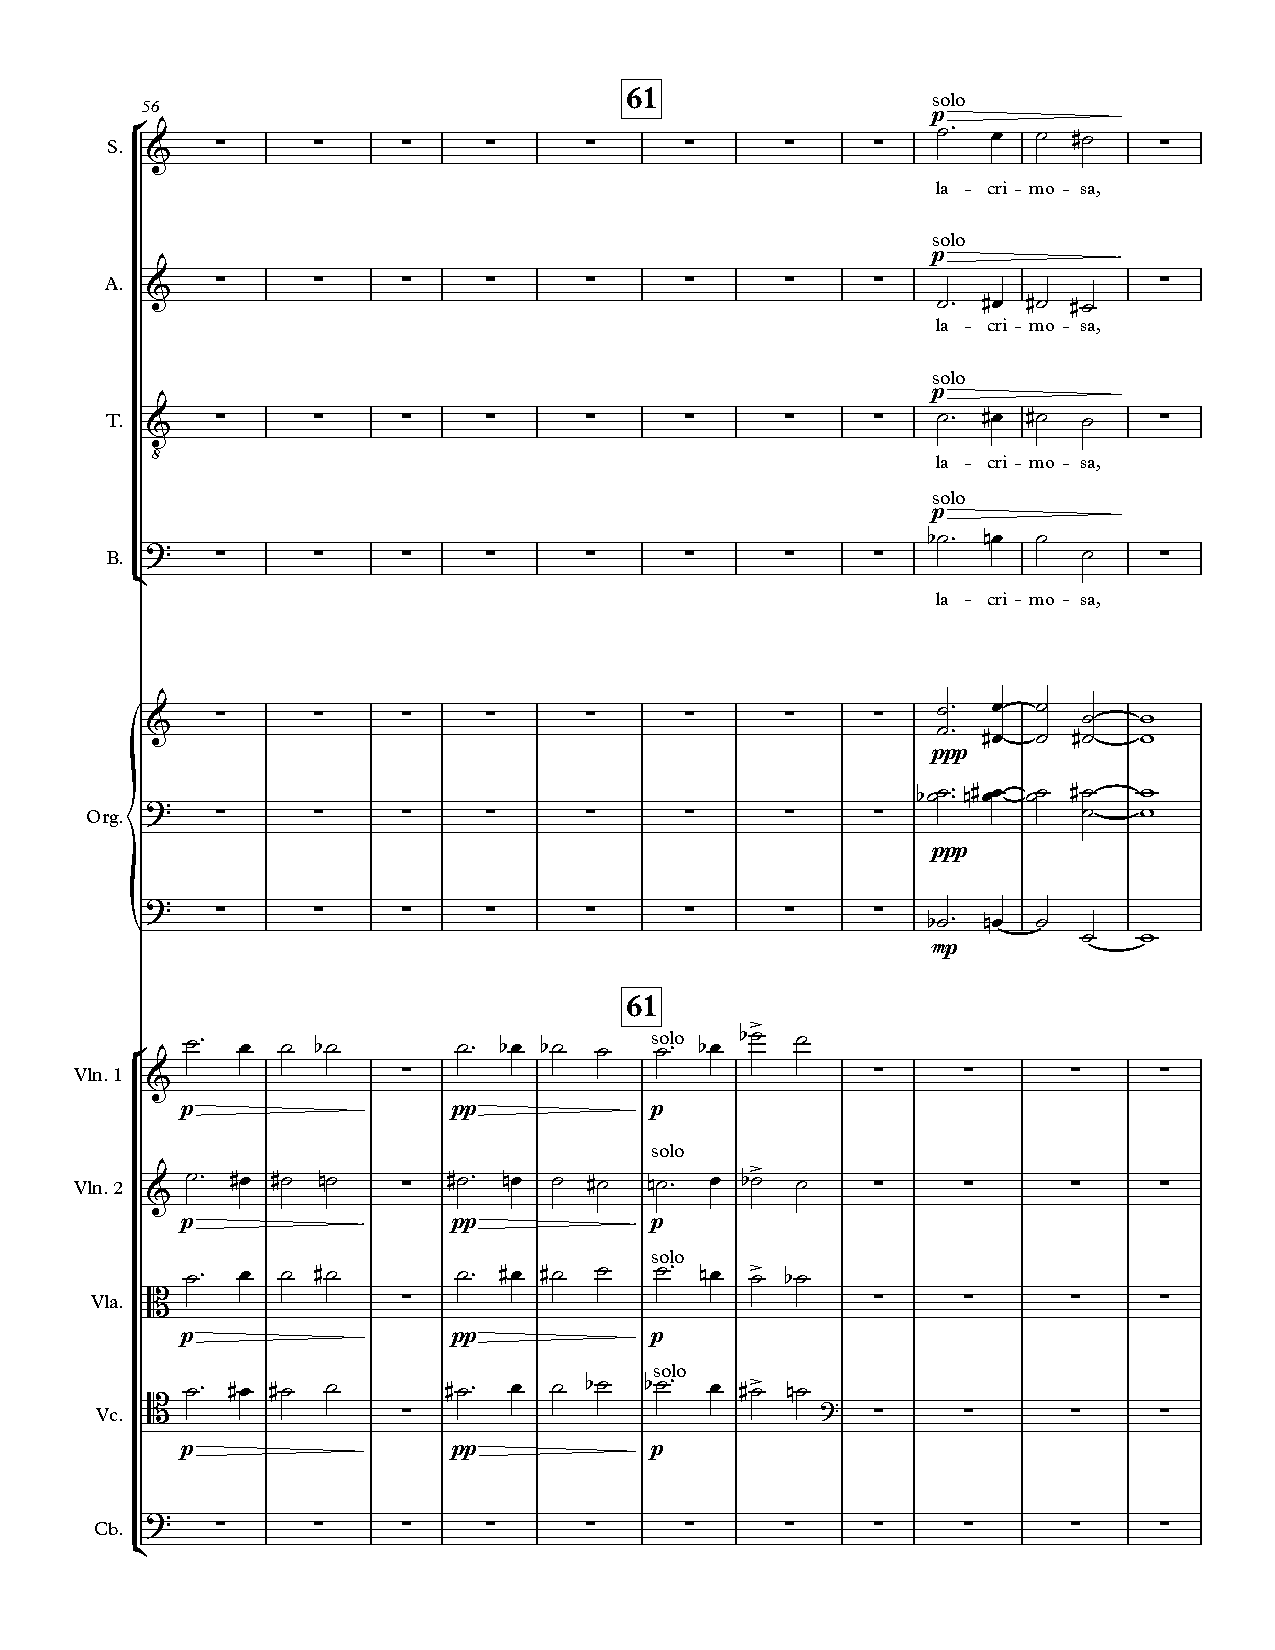
\includegraphics[width=6.5in]{figures/Stabat_Mater_12.pdf}
\end{figure}

%--------------------------------------------------------------------------
\begin{figure}[htbp]
    \centering
	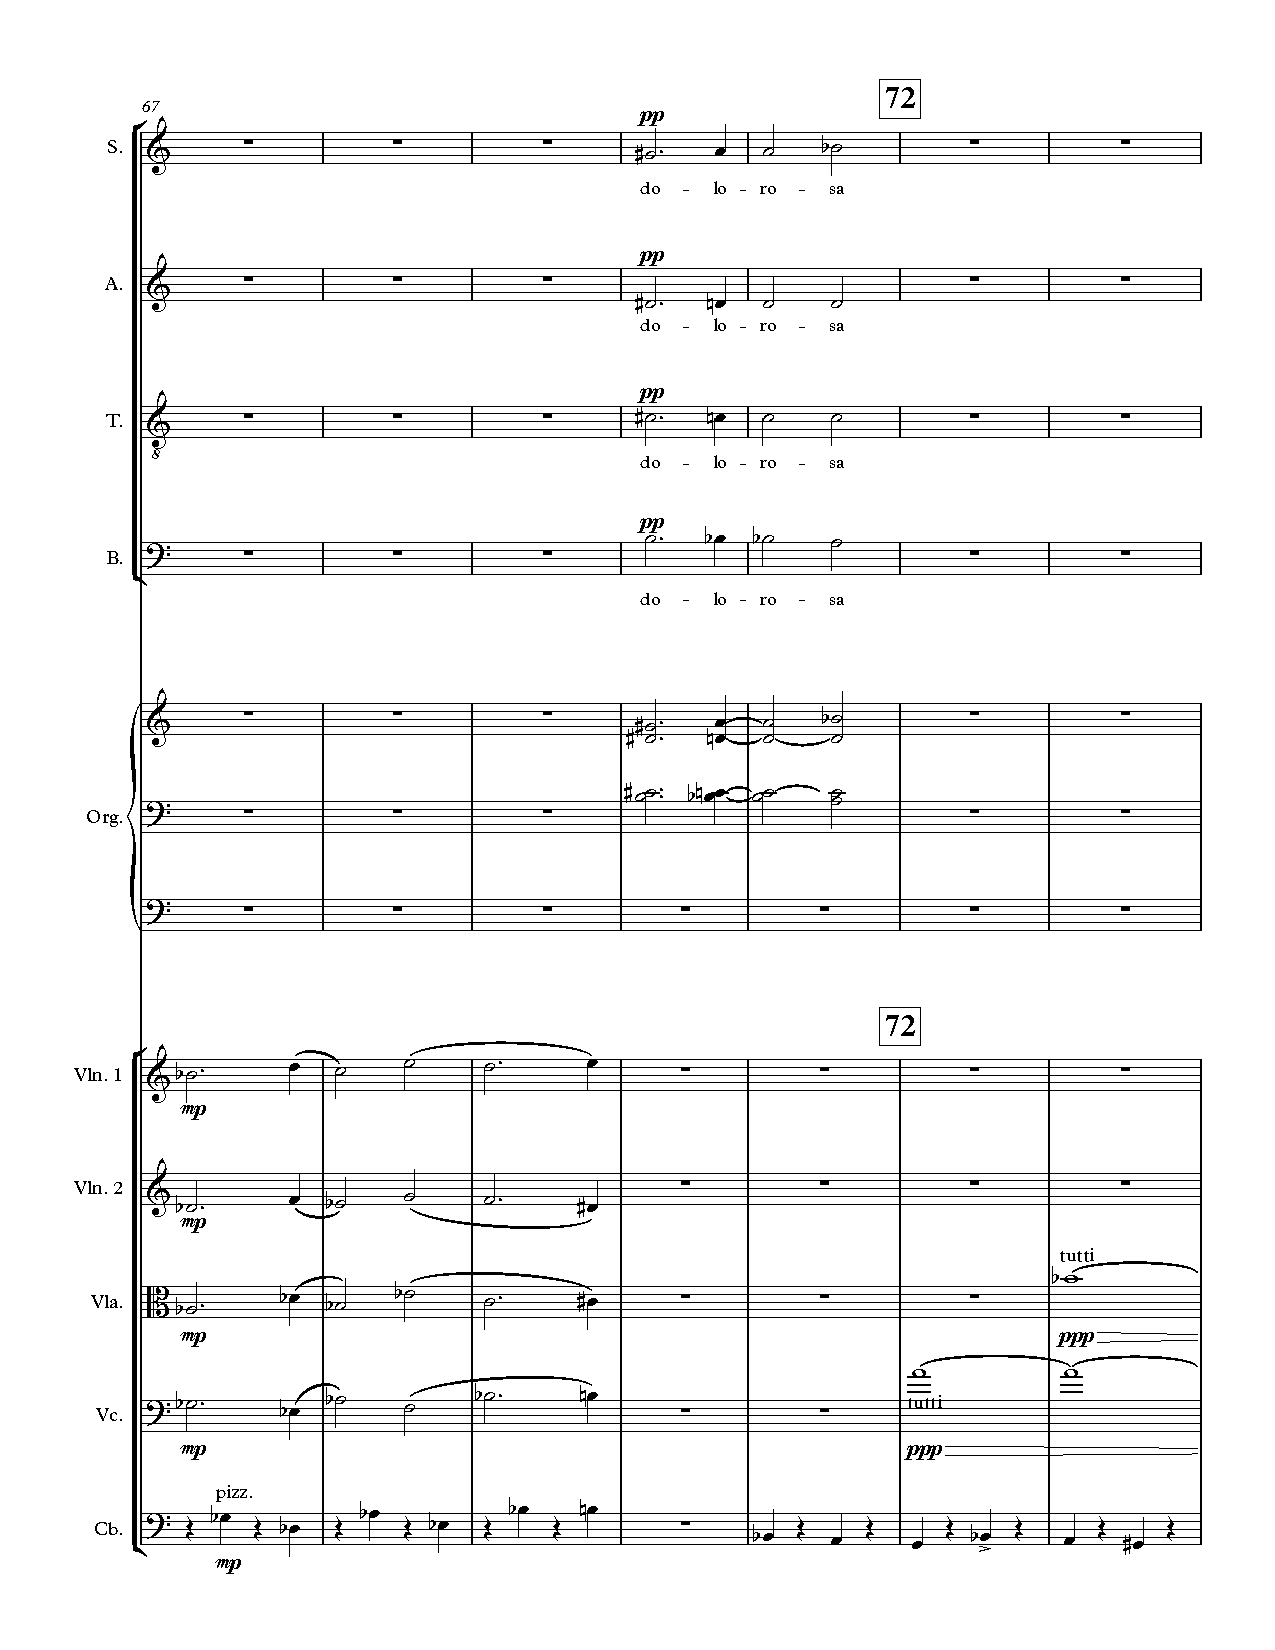
\includegraphics[width=6.5in]{figures/Stabat_Mater_13.pdf}
\end{figure}

%--------------------------------------------------------------------------
\begin{figure}[htbp]
    \centering
	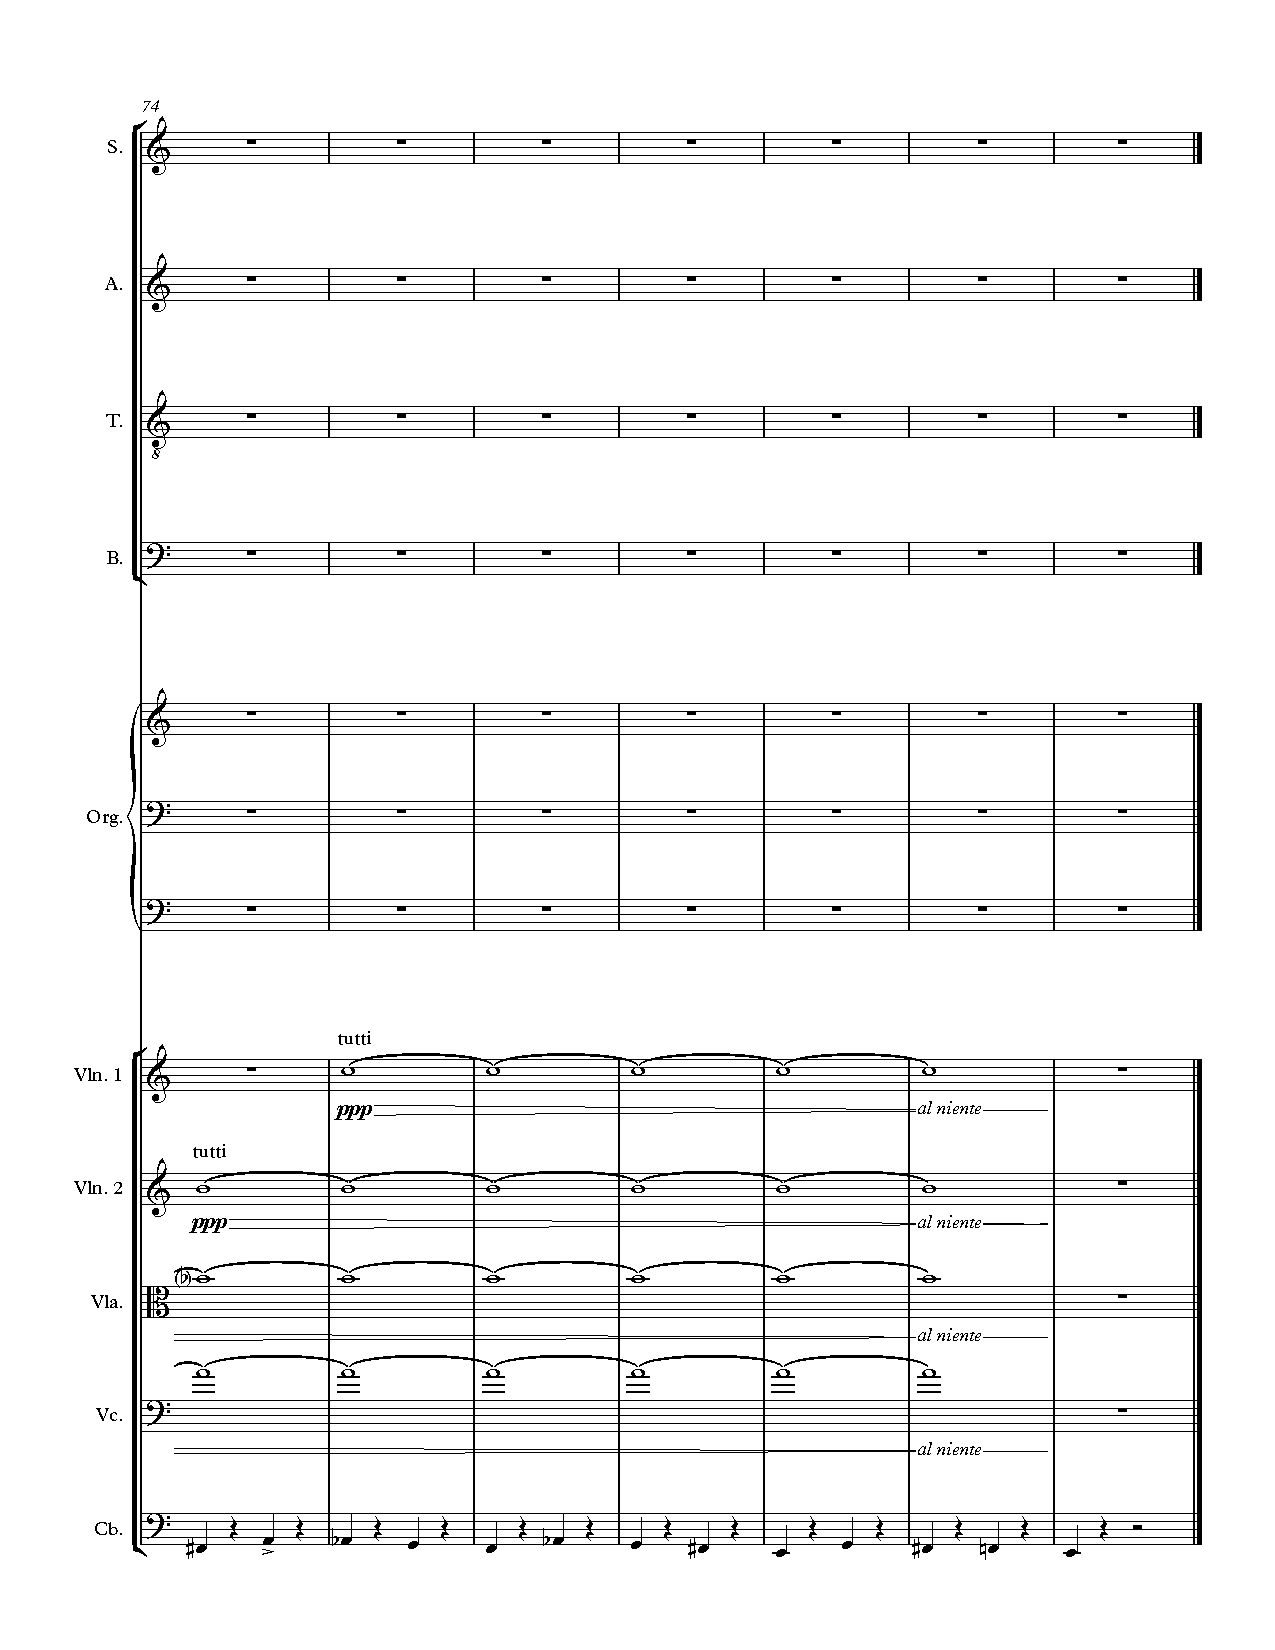
\includegraphics[width=6.5in]{figures/Stabat_Mater_14.pdf}
\end{figure}

%--------------------------------------------------------------------------
\section{Program Notes}

%--------------------------------------------------------------------------
\emph{Stabat Mater} is a piece for SATB choir, organ and string orchestra. It is (very) loosely inspired by the Stabat Mater of Pergolesi, and perhaps a bit by the second movement of the String Quartet No. 4 of Bart\'{o}k. The piece is constructed around a concept of smooth voice-leading, where each harmonic set is morphed into the next with the absolute minimum amount of motion in each voice. The syntax of these motions is structured around simple antecedent-consequent periods, connected by sequential developments to form phrases. The orchestra opens the piece with a turbulent presentation, simbolizing the clamor of the crowds, along with the heavy steps of the \emph{via crucis}, whereas choir and organ personify the suffering and transcendence of mother and son.

%--------------------------------------------------------------------------
\chapter{Out of Focus for Wind Quintet}
\vspace{-2em}

%--------------------------------------------------------------------------
\begin{figure}[H]
    \centering
	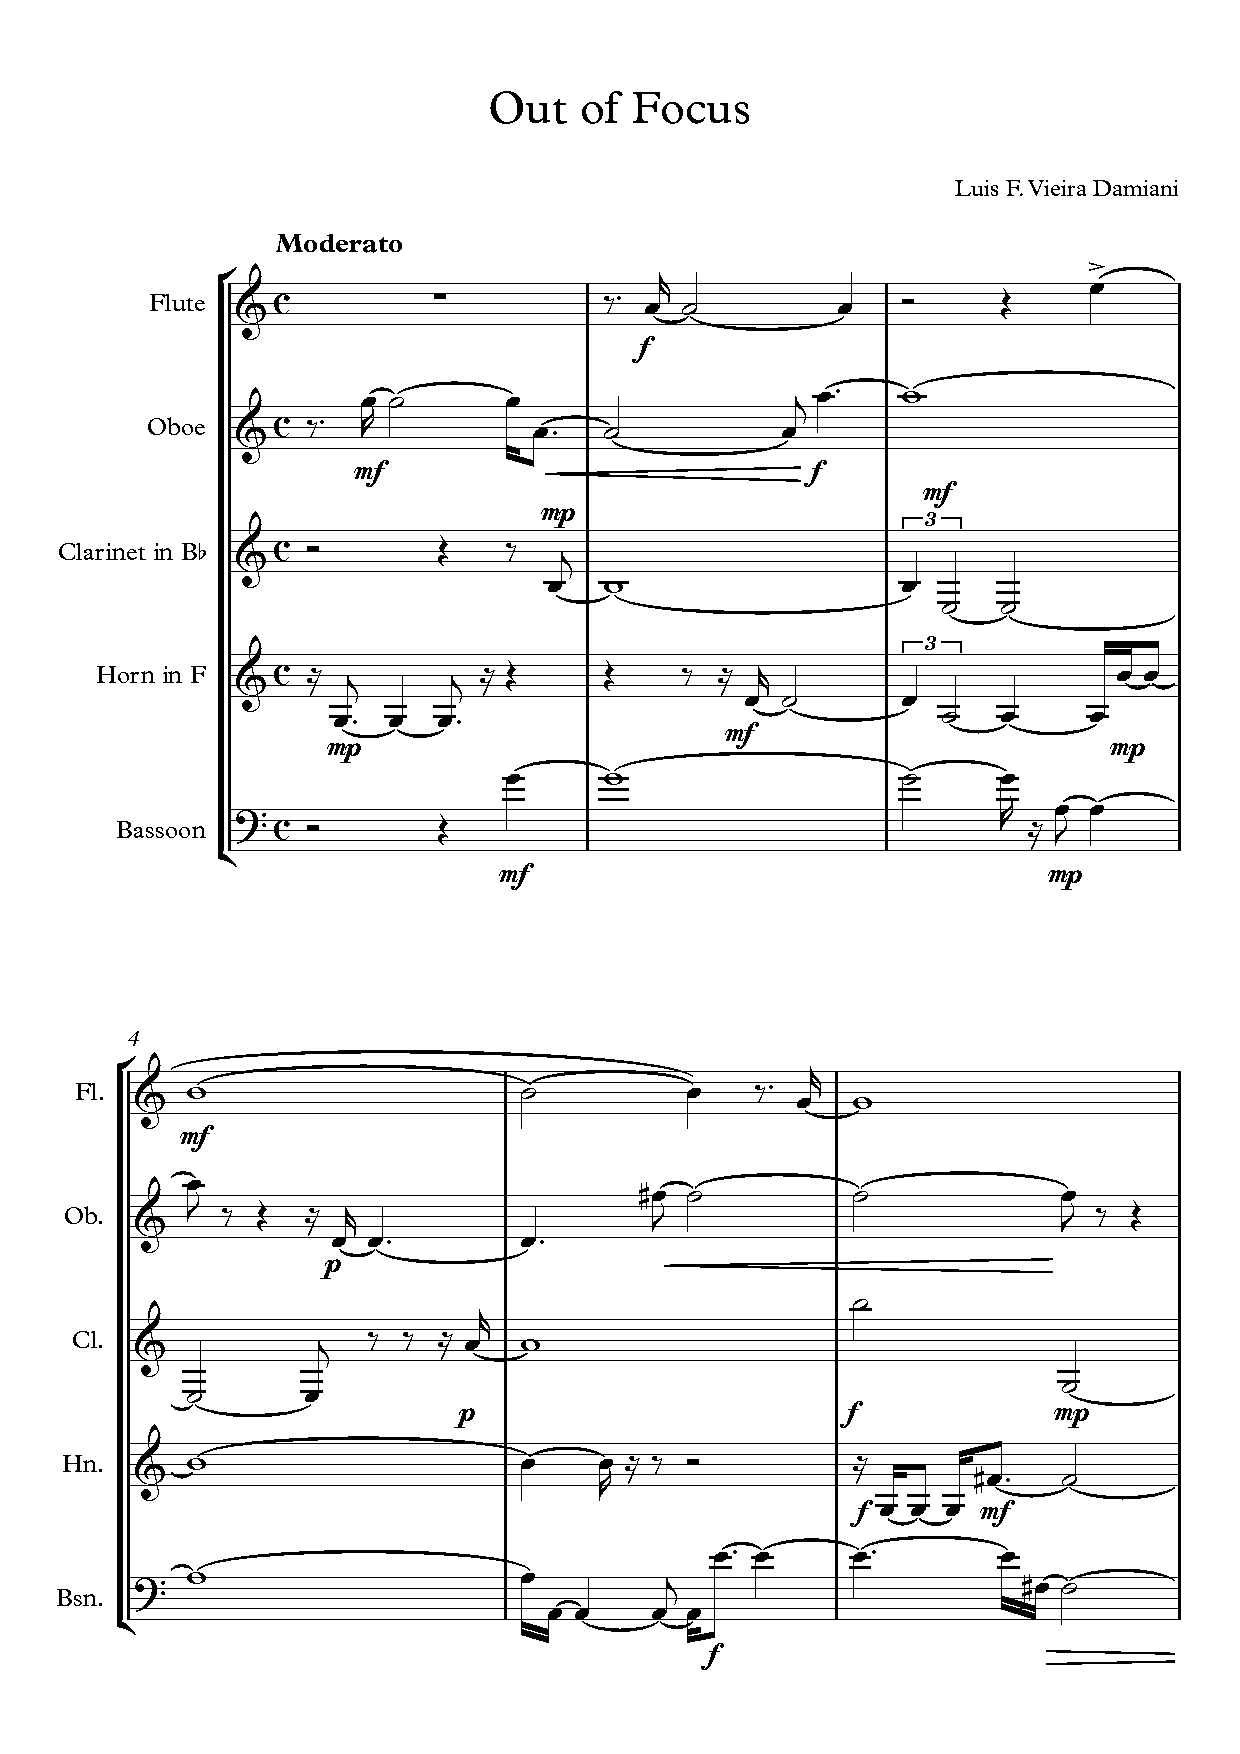
\includegraphics[width=6.5in]{figures/Out_of_Focus_1.pdf}
\end{figure}

%--------------------------------------------------------------------------
\begin{figure}[H]
    \centering
	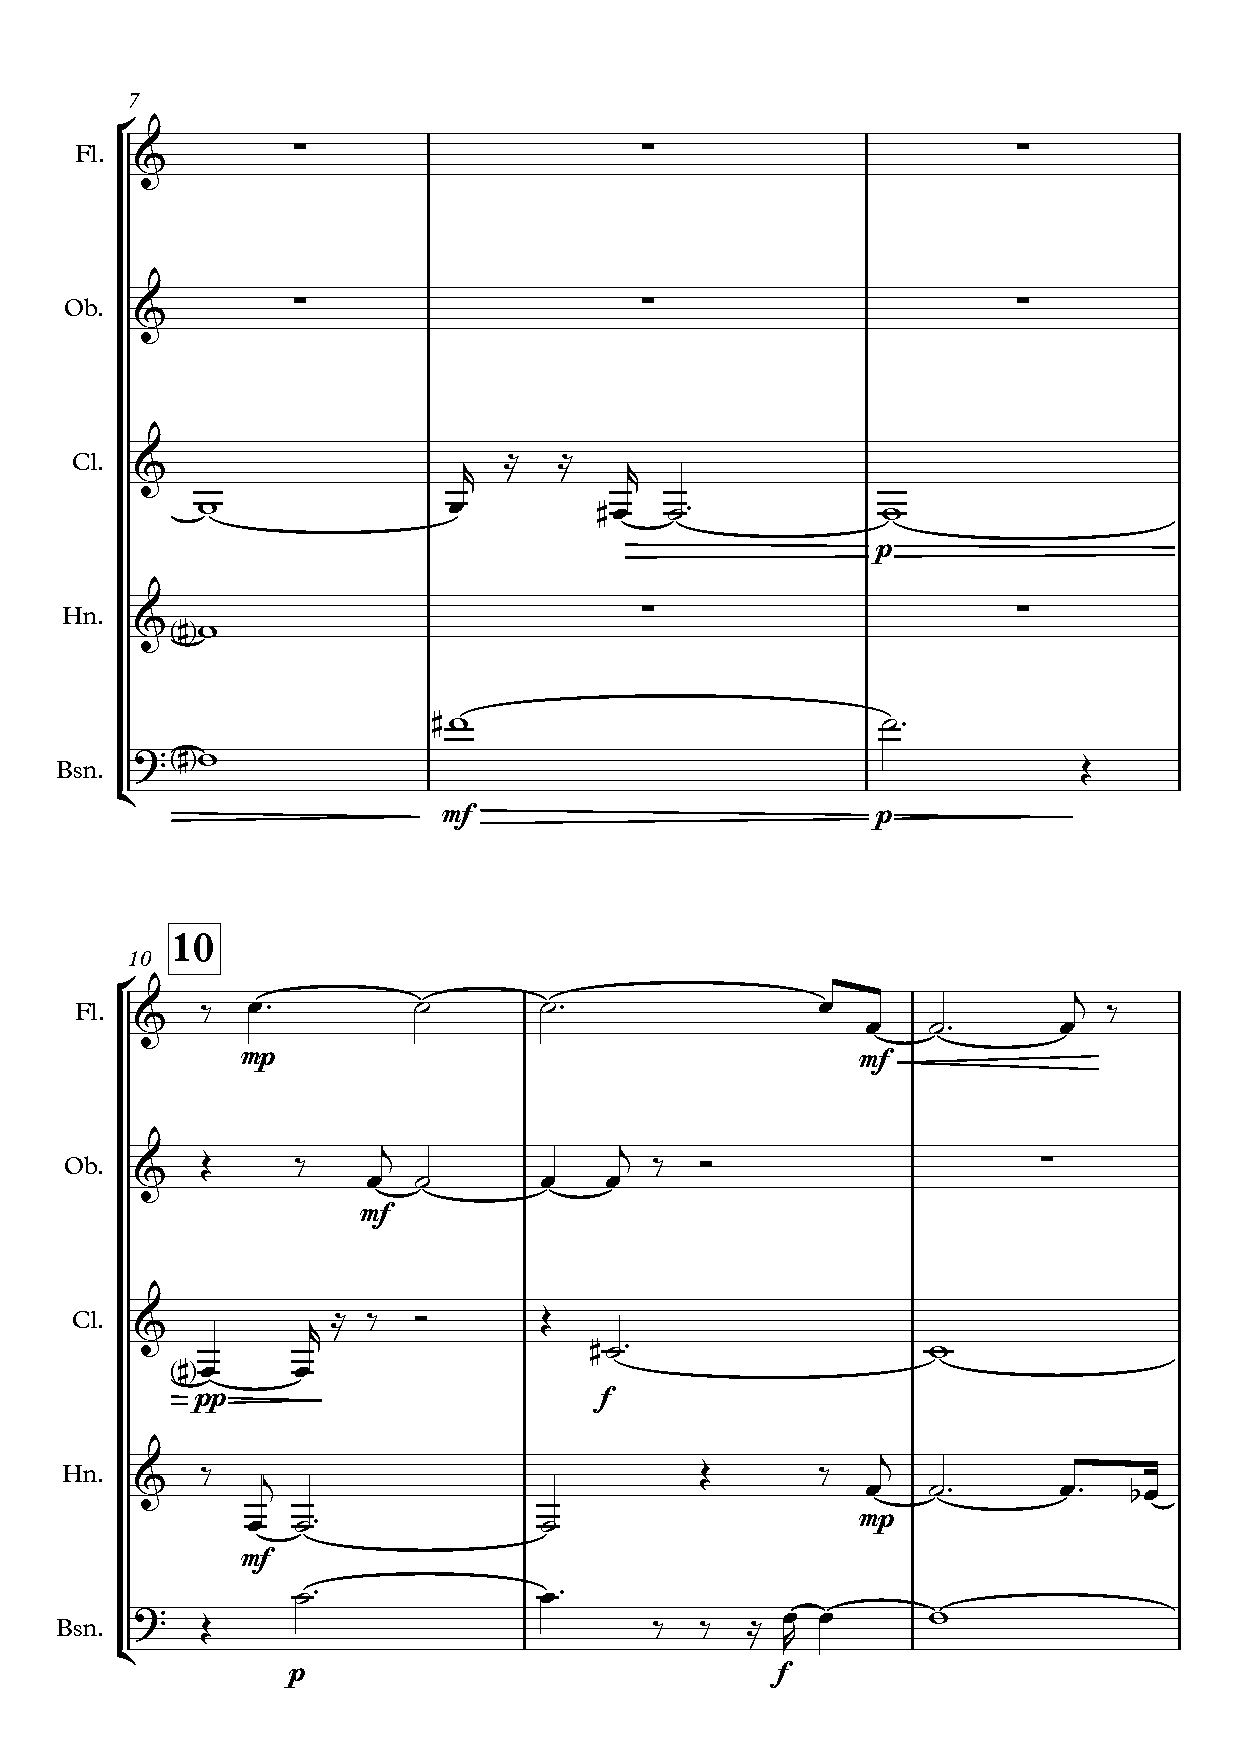
\includegraphics[width=6.5in]{figures/Out_of_Focus_2.pdf}
\end{figure}

%--------------------------------------------------------------------------
\begin{figure}[H]
    \centering
	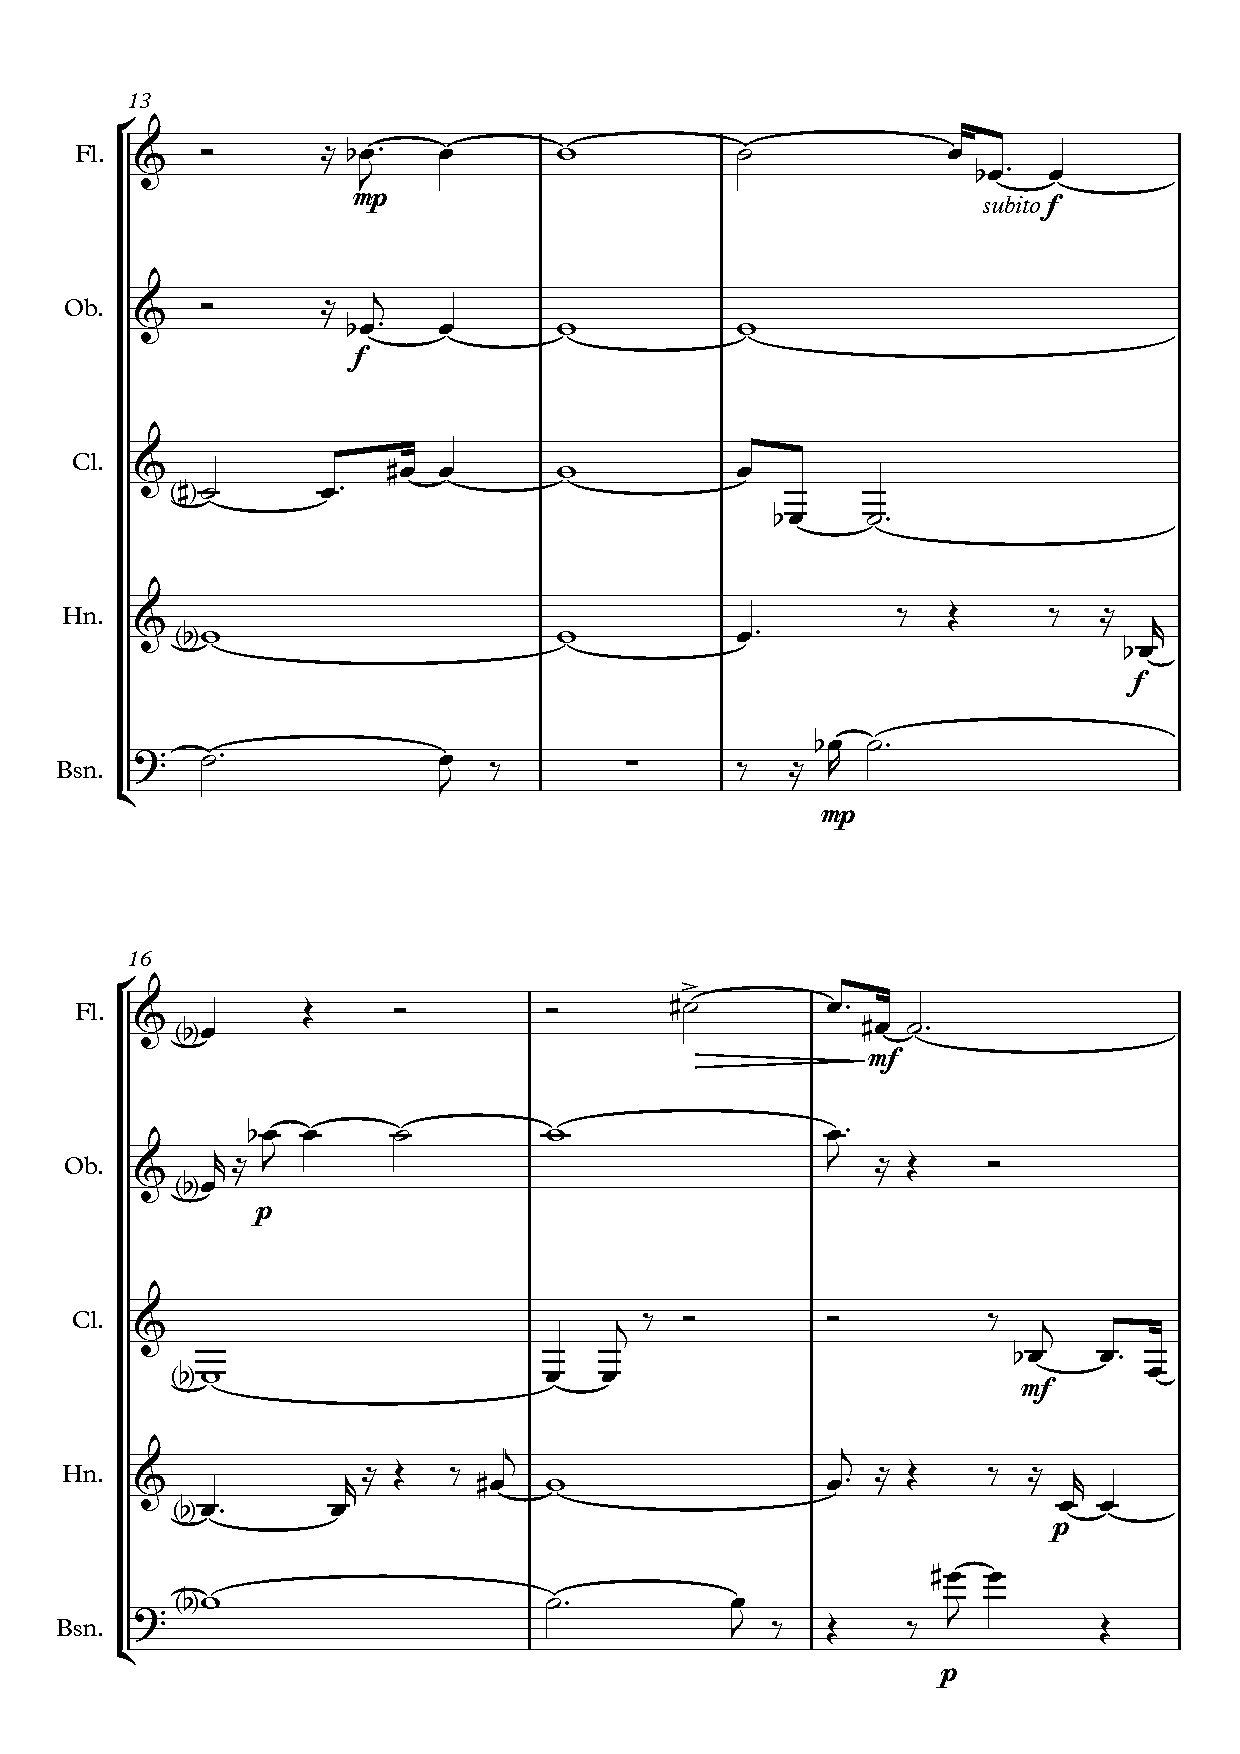
\includegraphics[width=6.5in]{figures/Out_of_Focus_3.pdf}
\end{figure}

%--------------------------------------------------------------------------
\begin{figure}[H]
    \centering
	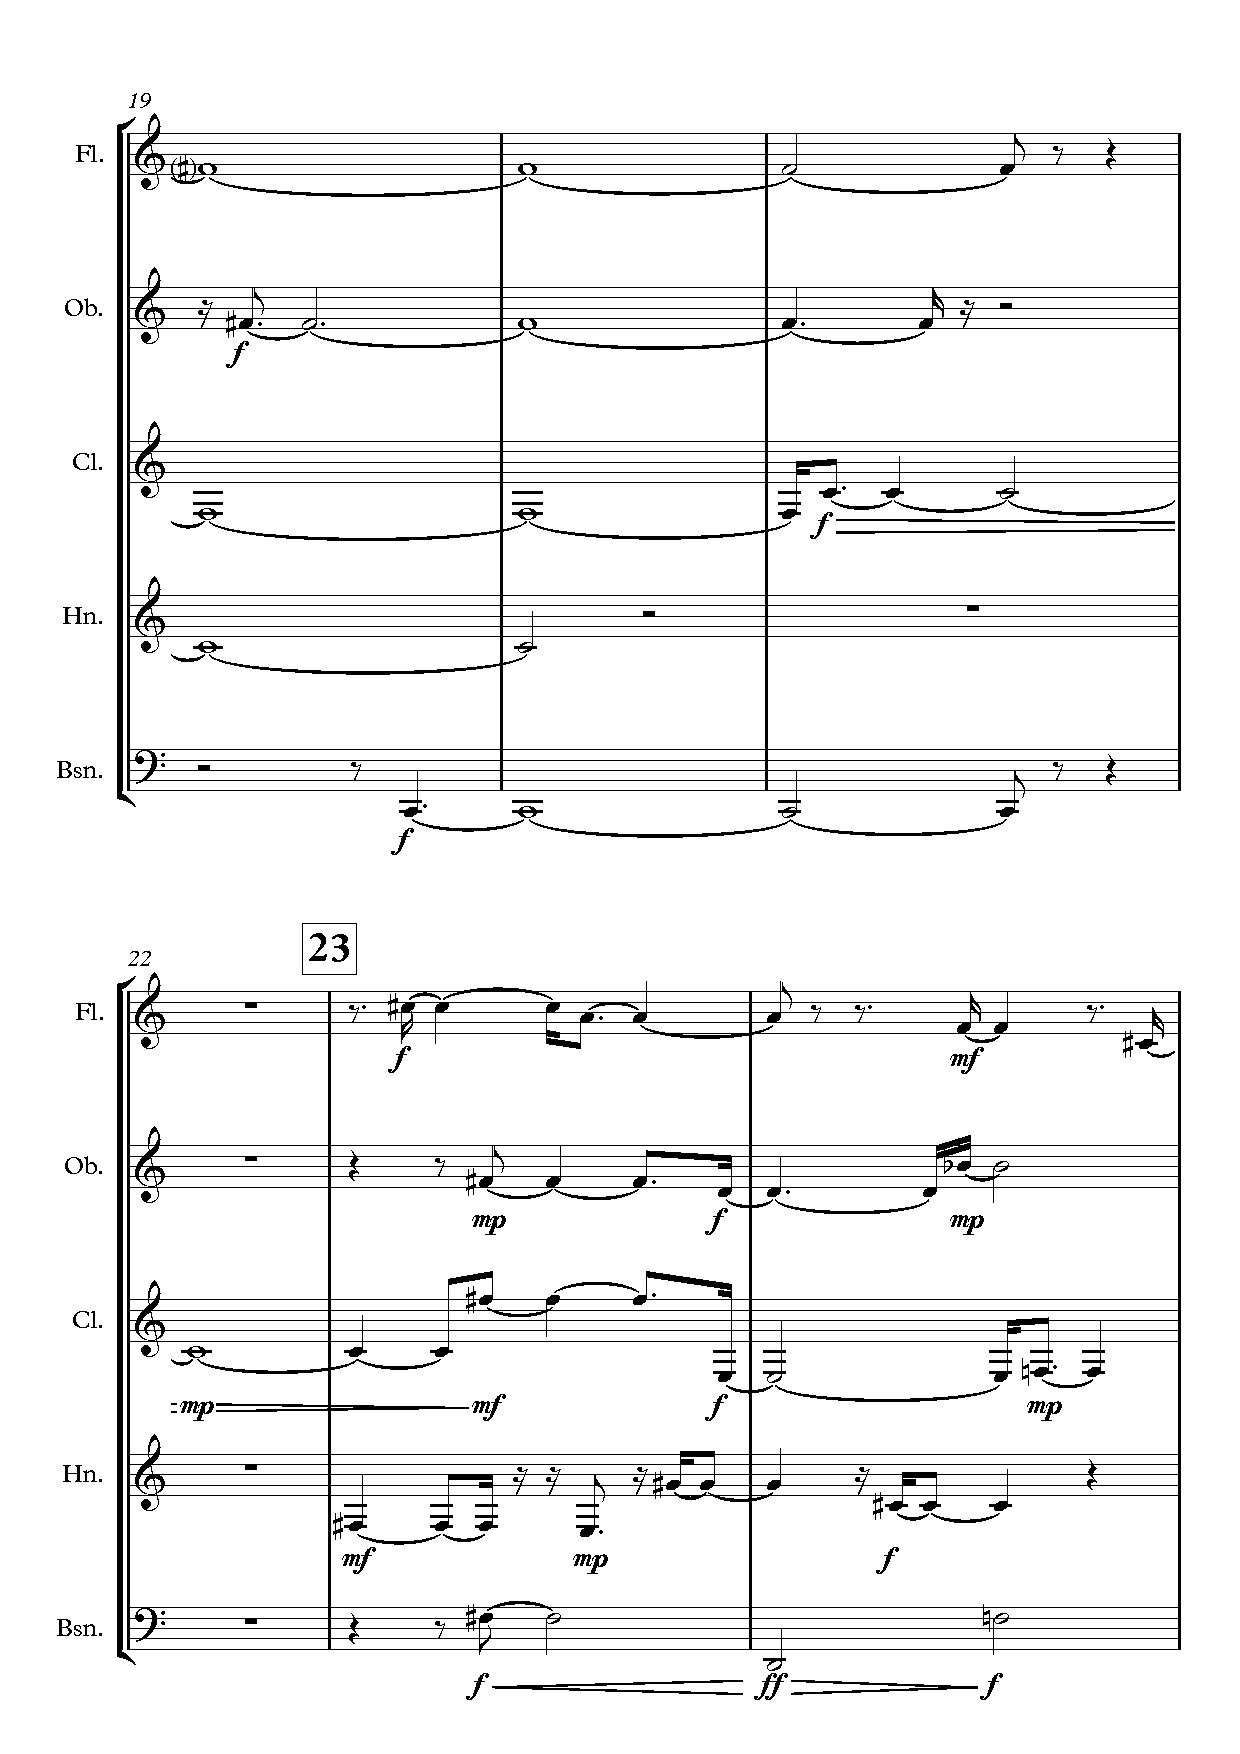
\includegraphics[width=6.5in]{figures/Out_of_Focus_4.pdf}
\end{figure}

%--------------------------------------------------------------------------
\begin{figure}[H]
    \centering
	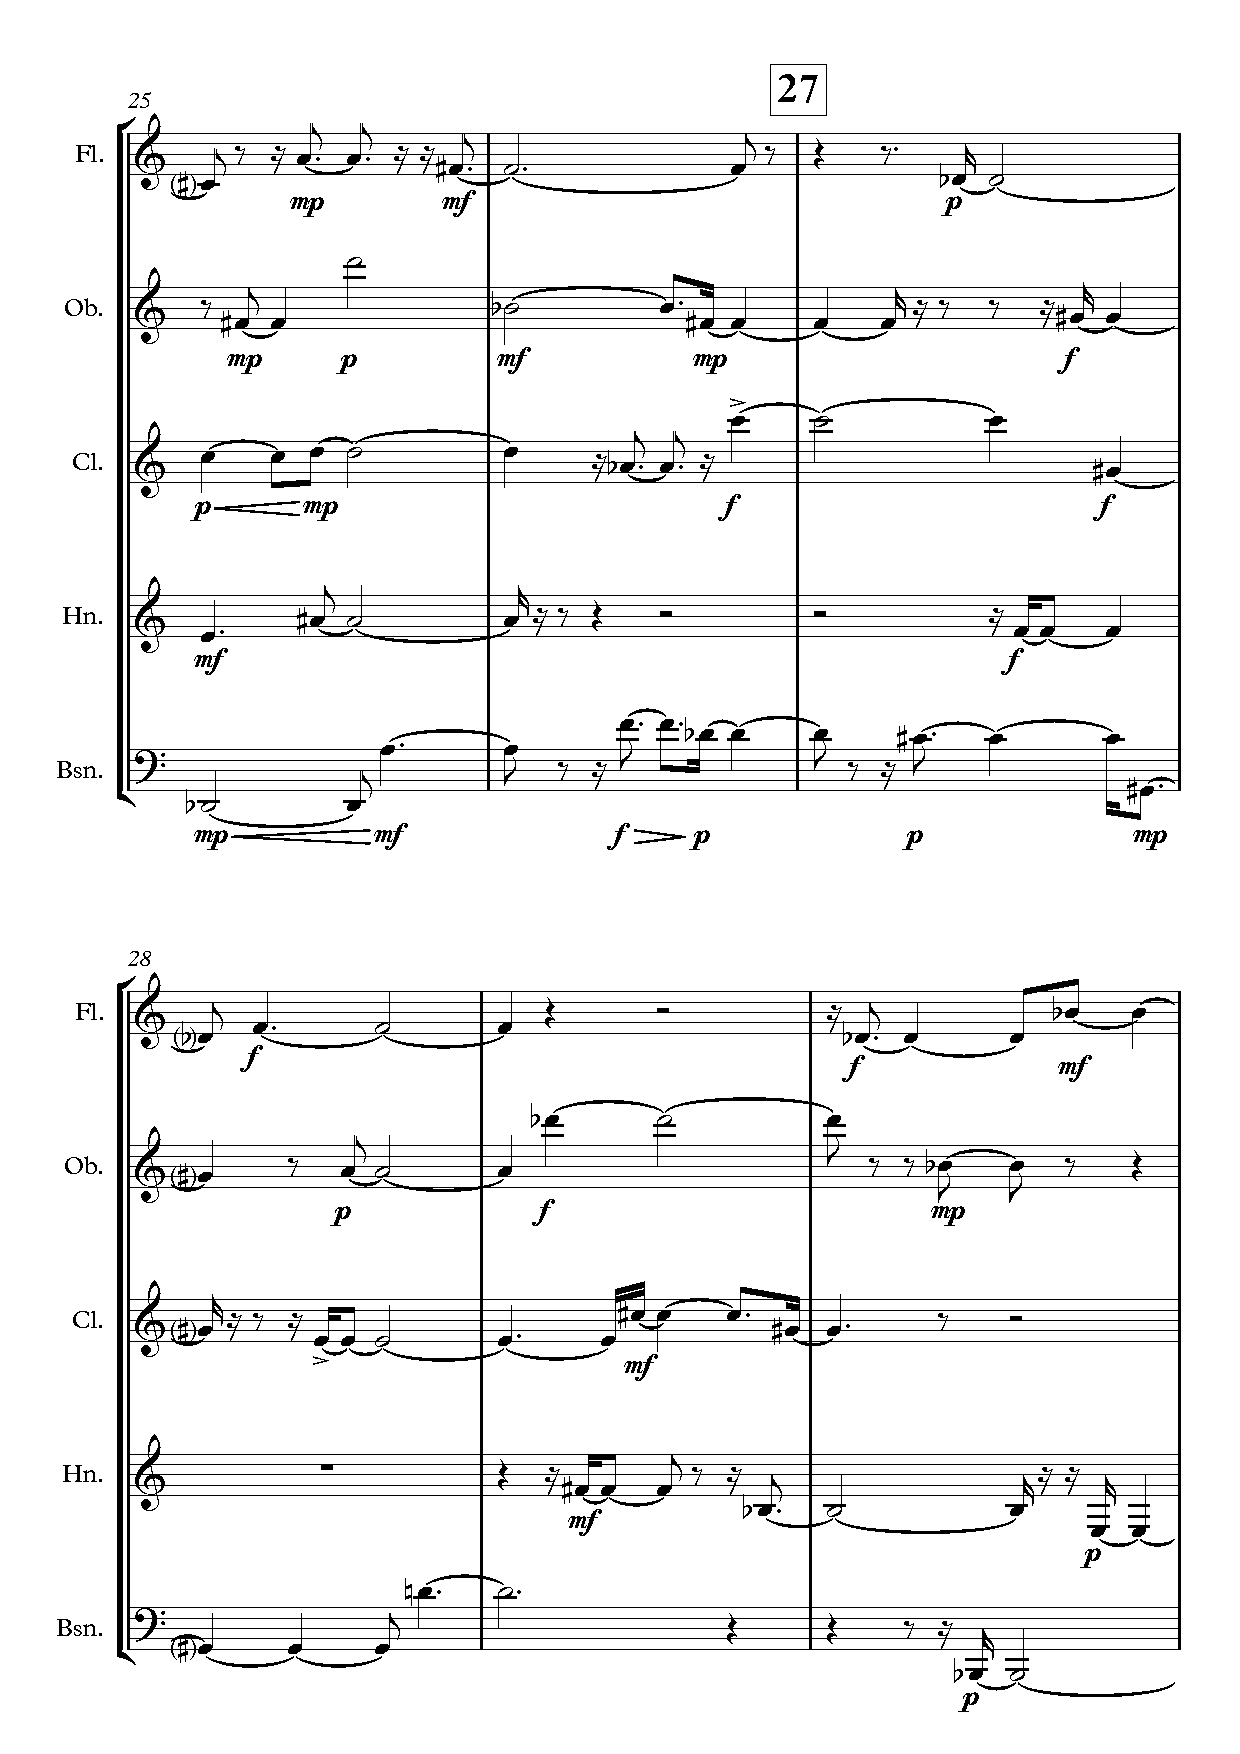
\includegraphics[width=6.5in]{figures/Out_of_Focus_5.pdf}
\end{figure}

%--------------------------------------------------------------------------
\begin{figure}[H]
    \centering
	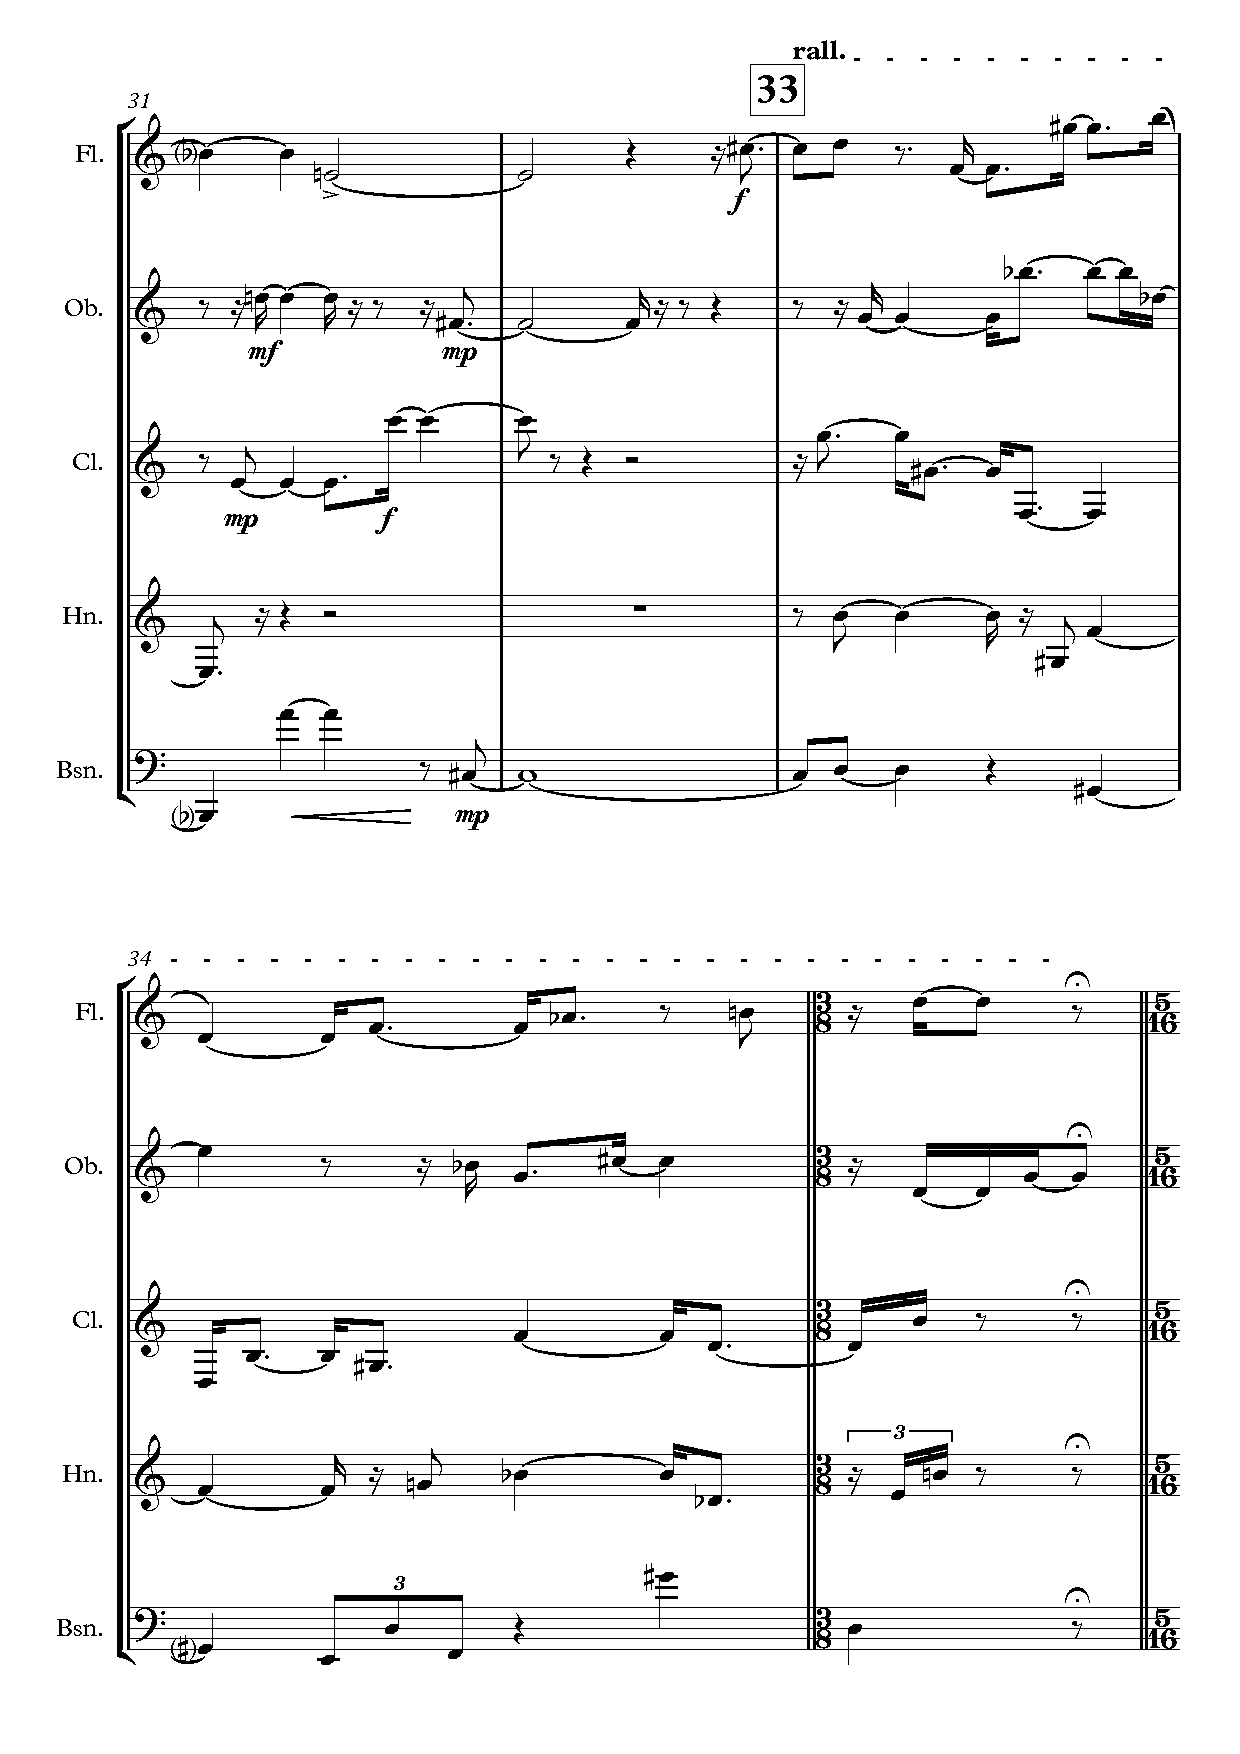
\includegraphics[width=6.5in]{figures/Out_of_Focus_6.pdf}
\end{figure}

%--------------------------------------------------------------------------
\begin{figure}[H]
    \centering
	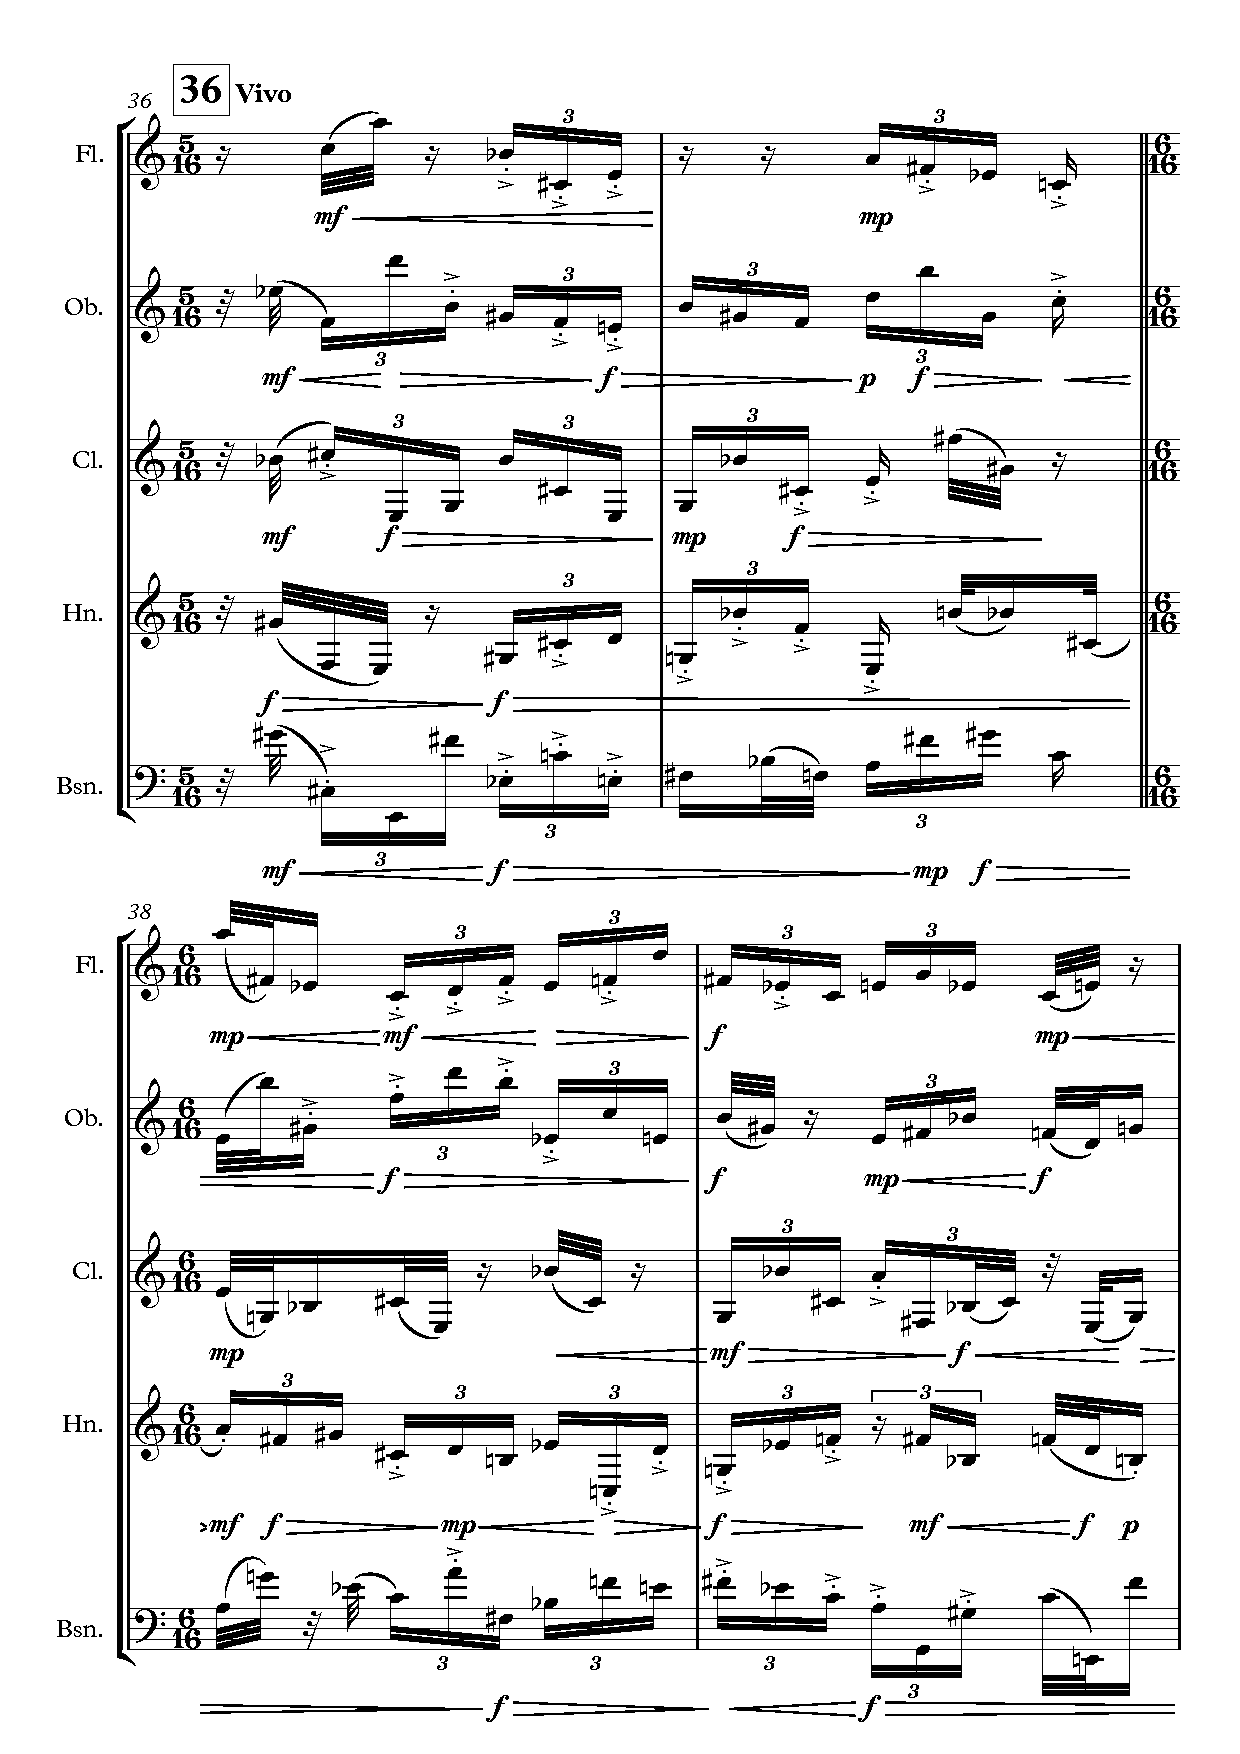
\includegraphics[width=6.5in]{figures/Out_of_Focus_7.pdf}
\end{figure}

%--------------------------------------------------------------------------
\begin{figure}[H]
    \centering
	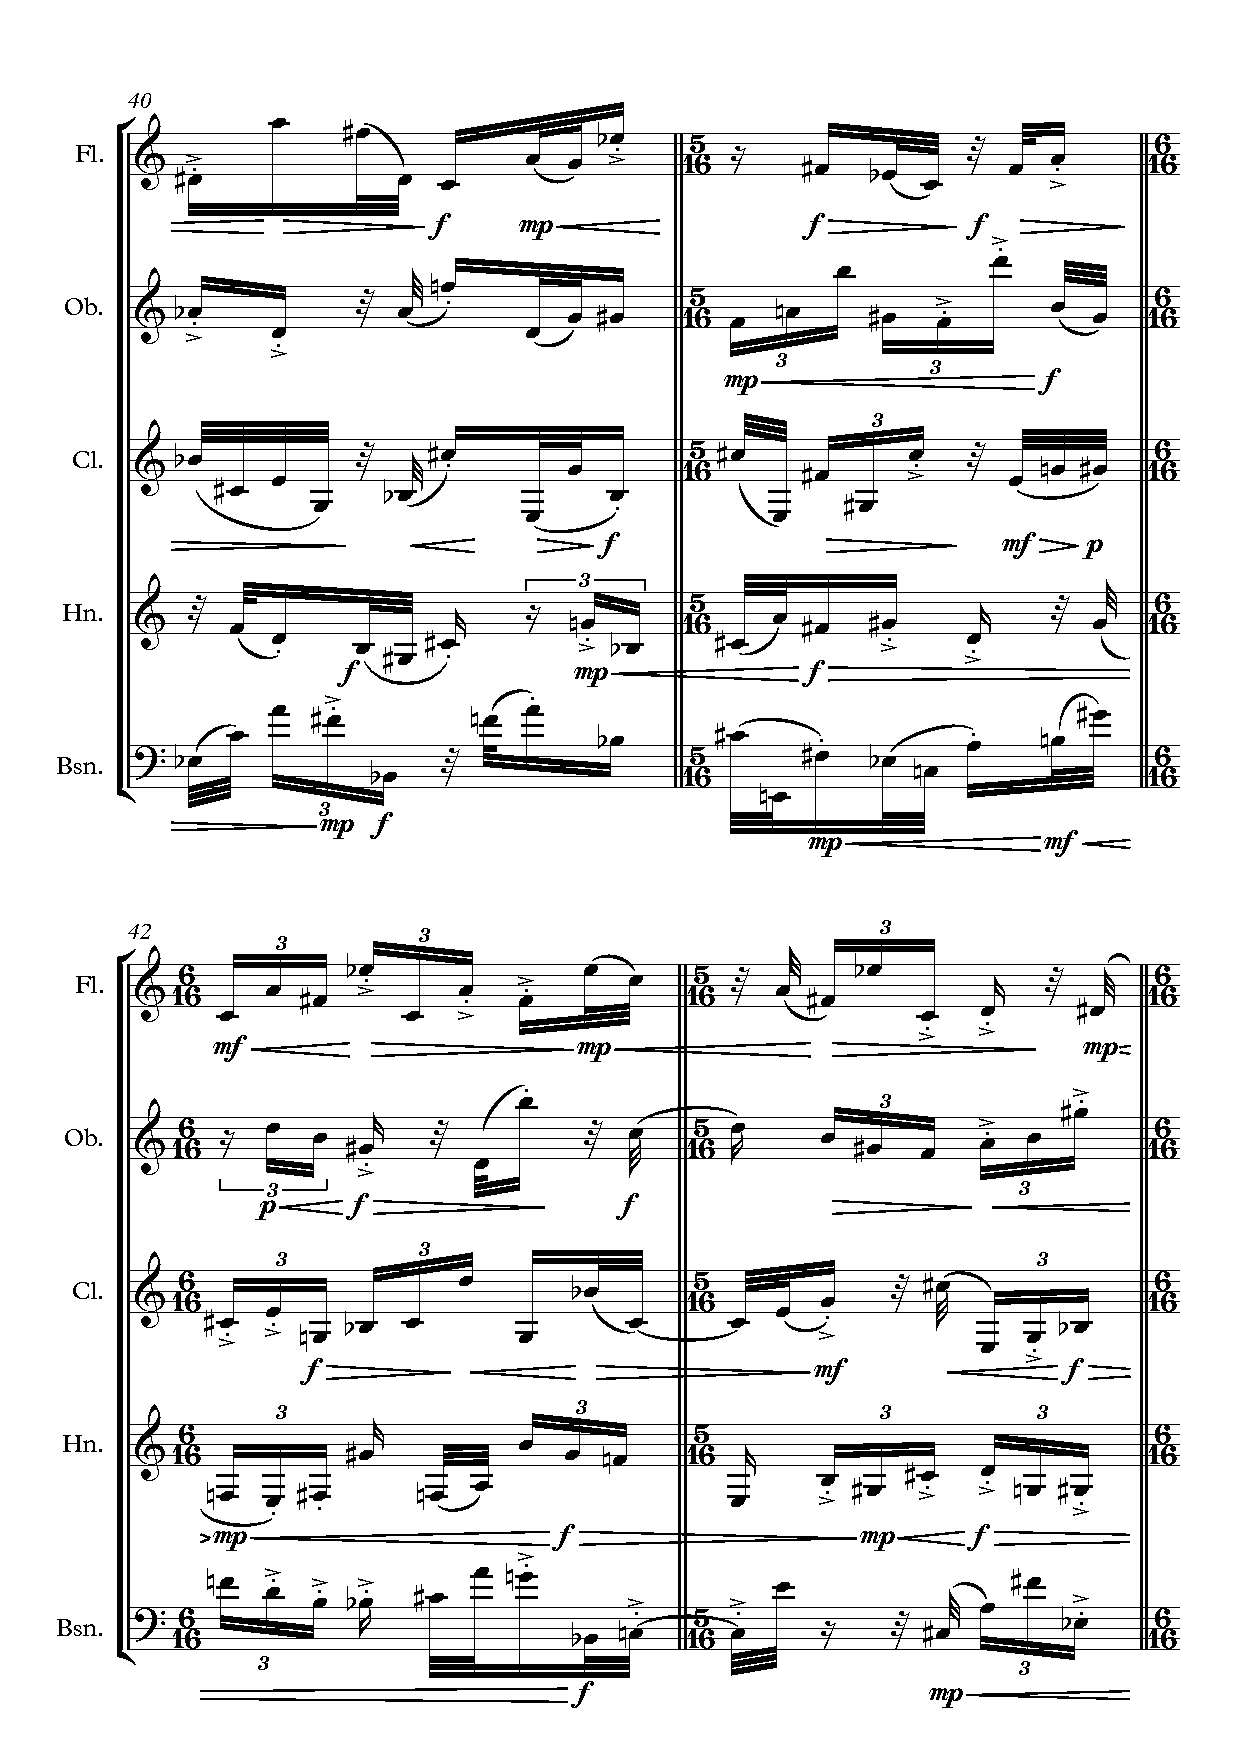
\includegraphics[width=6.5in]{figures/Out_of_Focus_8.pdf}
\end{figure}

%--------------------------------------------------------------------------
\begin{figure}[H]
    \centering
	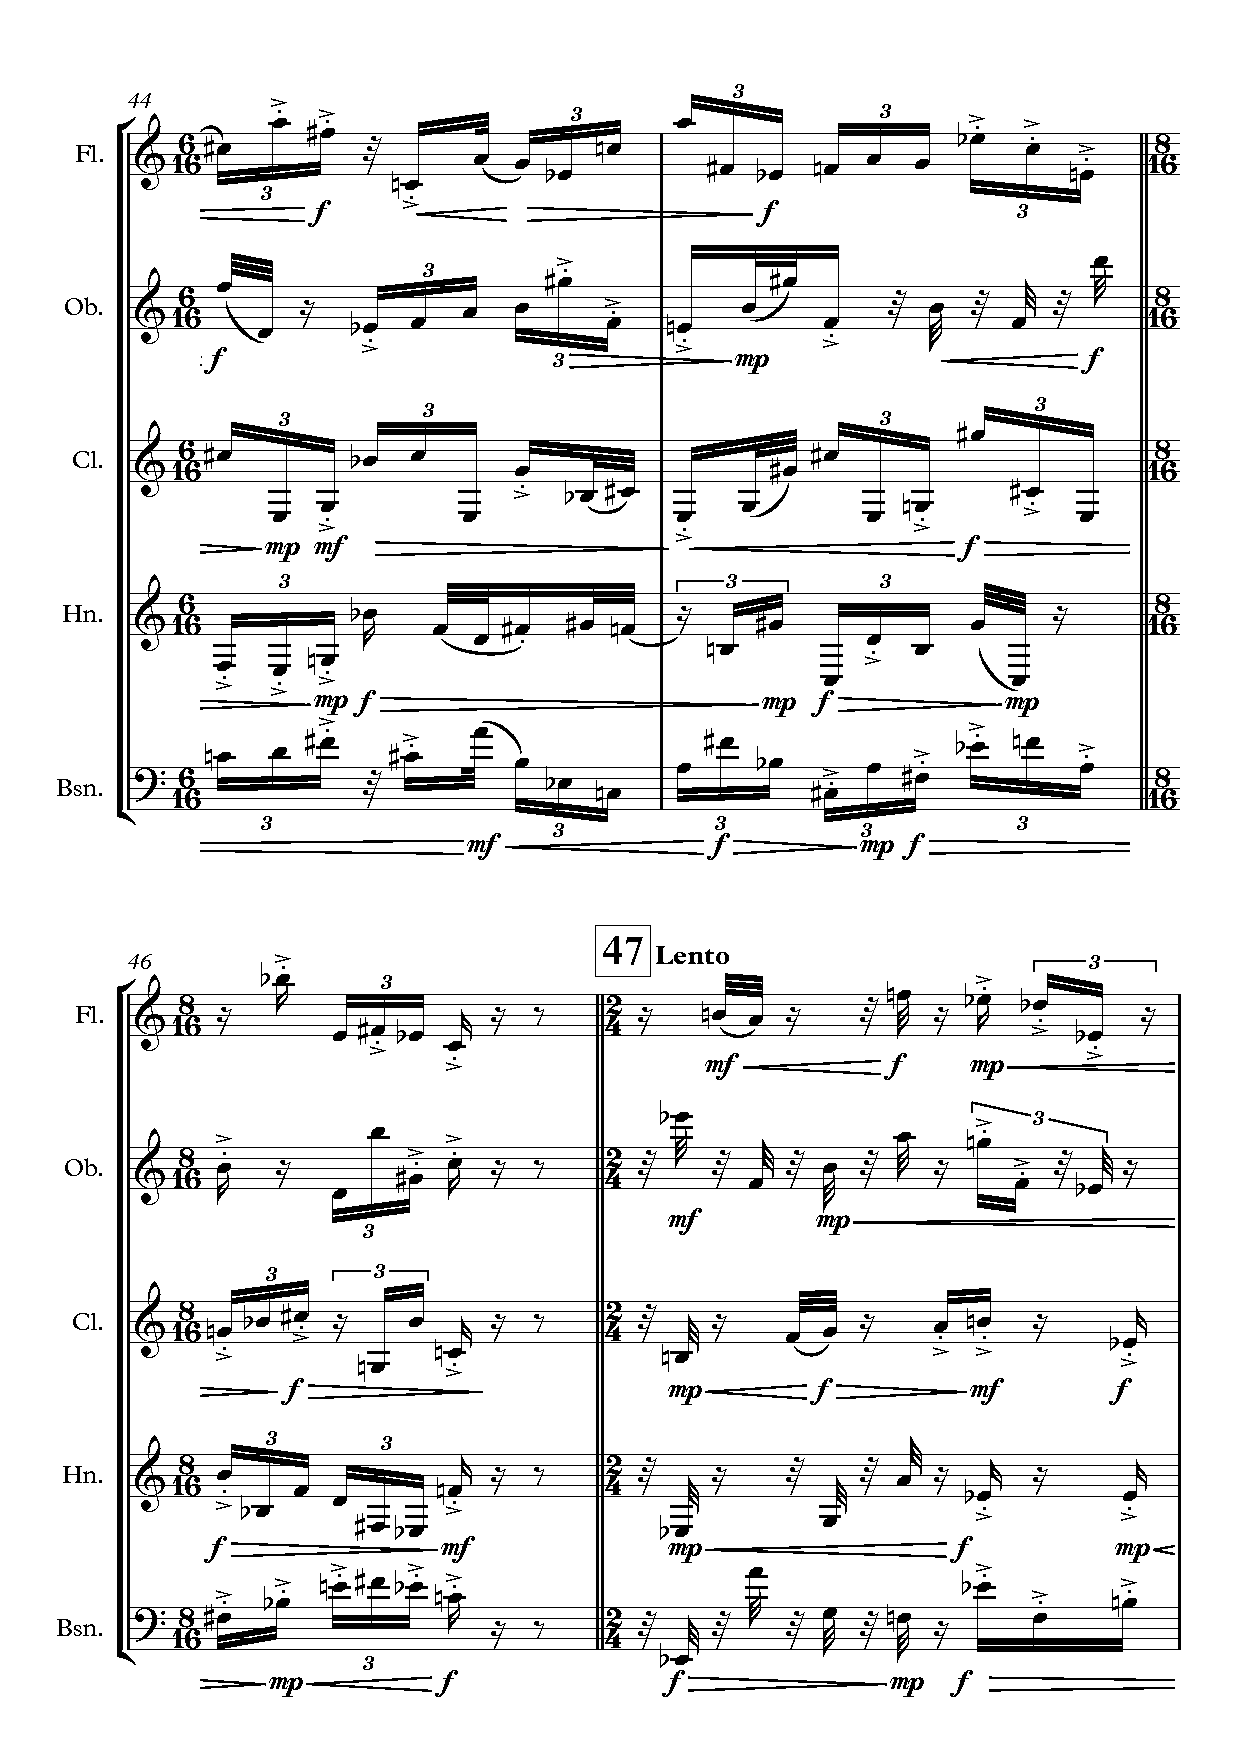
\includegraphics[width=6.5in]{figures/Out_of_Focus_9.pdf}
\end{figure}

%--------------------------------------------------------------------------
\begin{figure}[H]
    \centering
	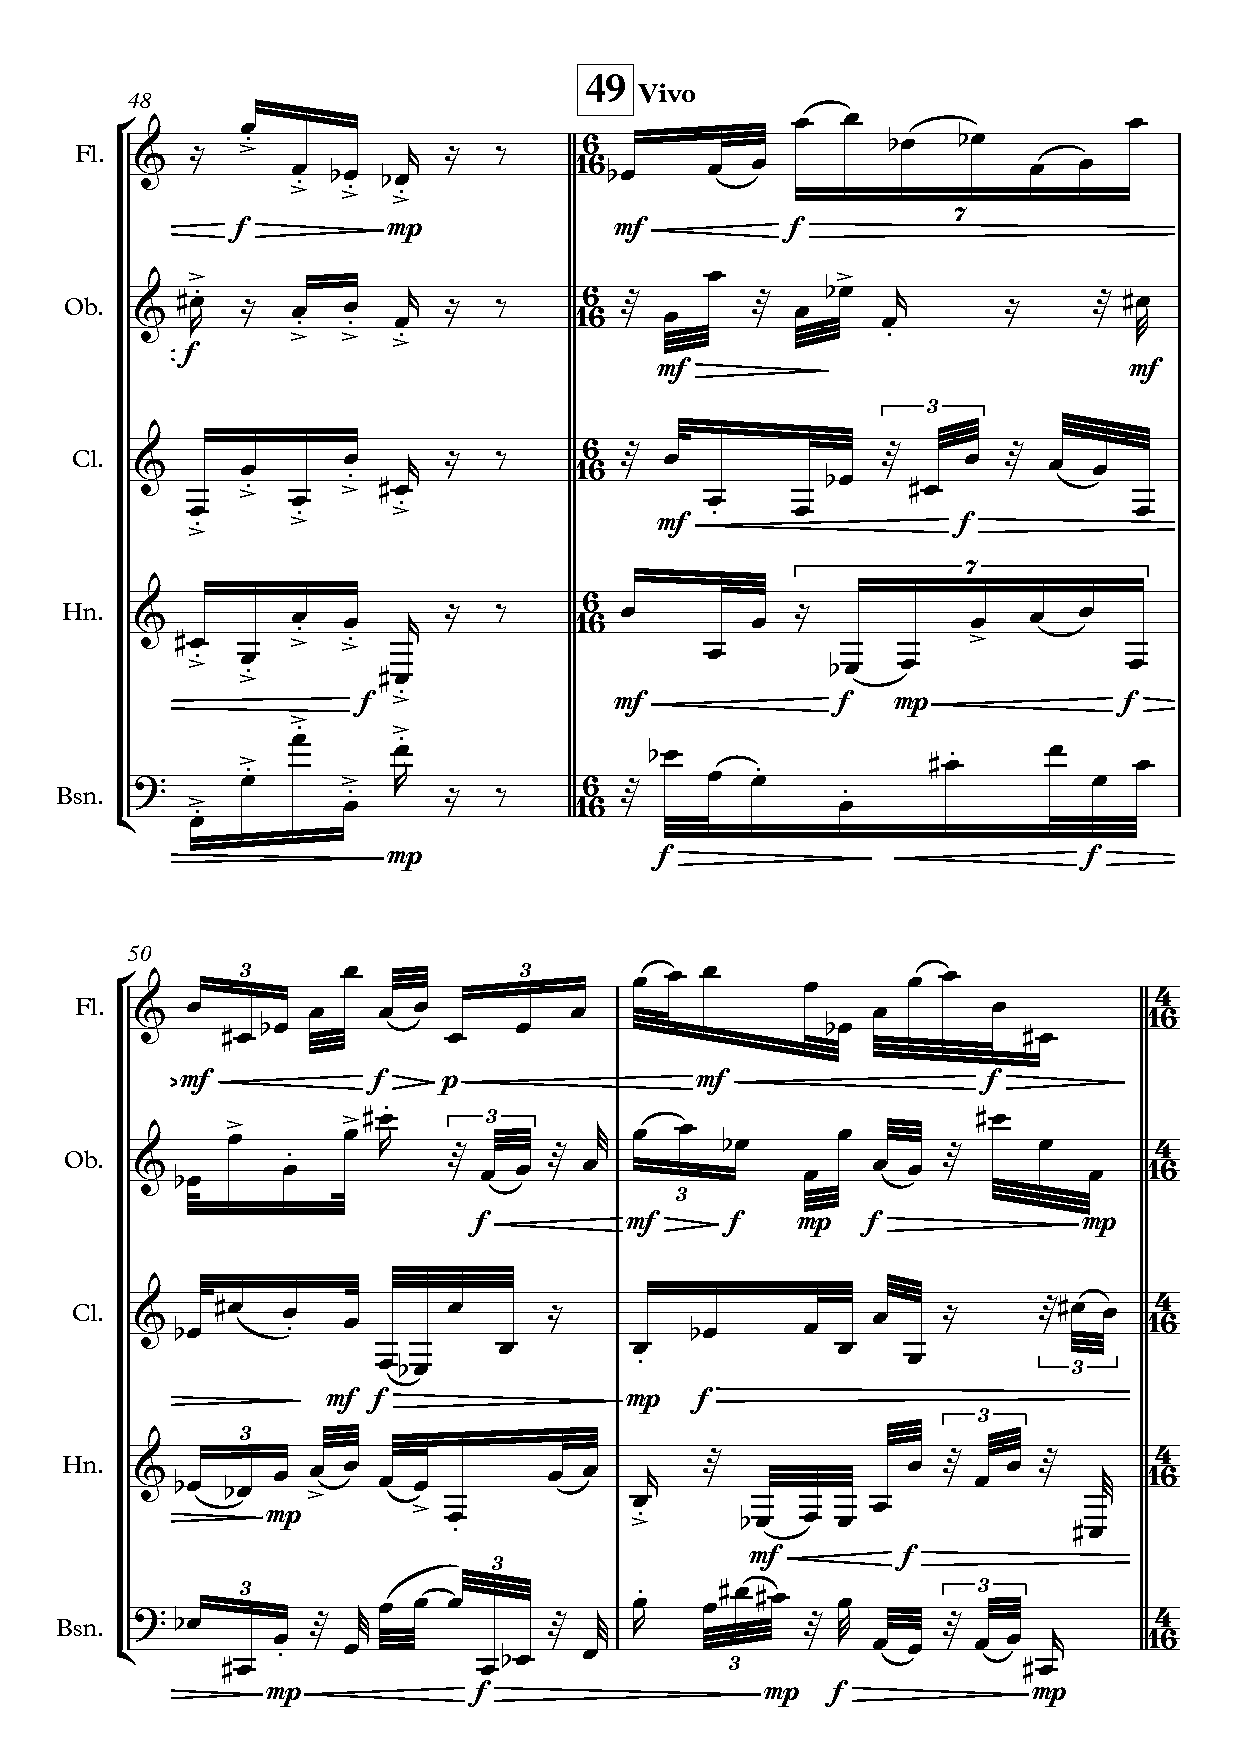
\includegraphics[width=6.5in]{figures/Out_of_Focus_10.pdf}
\end{figure}

%--------------------------------------------------------------------------
\begin{figure}[H]
    \centering
	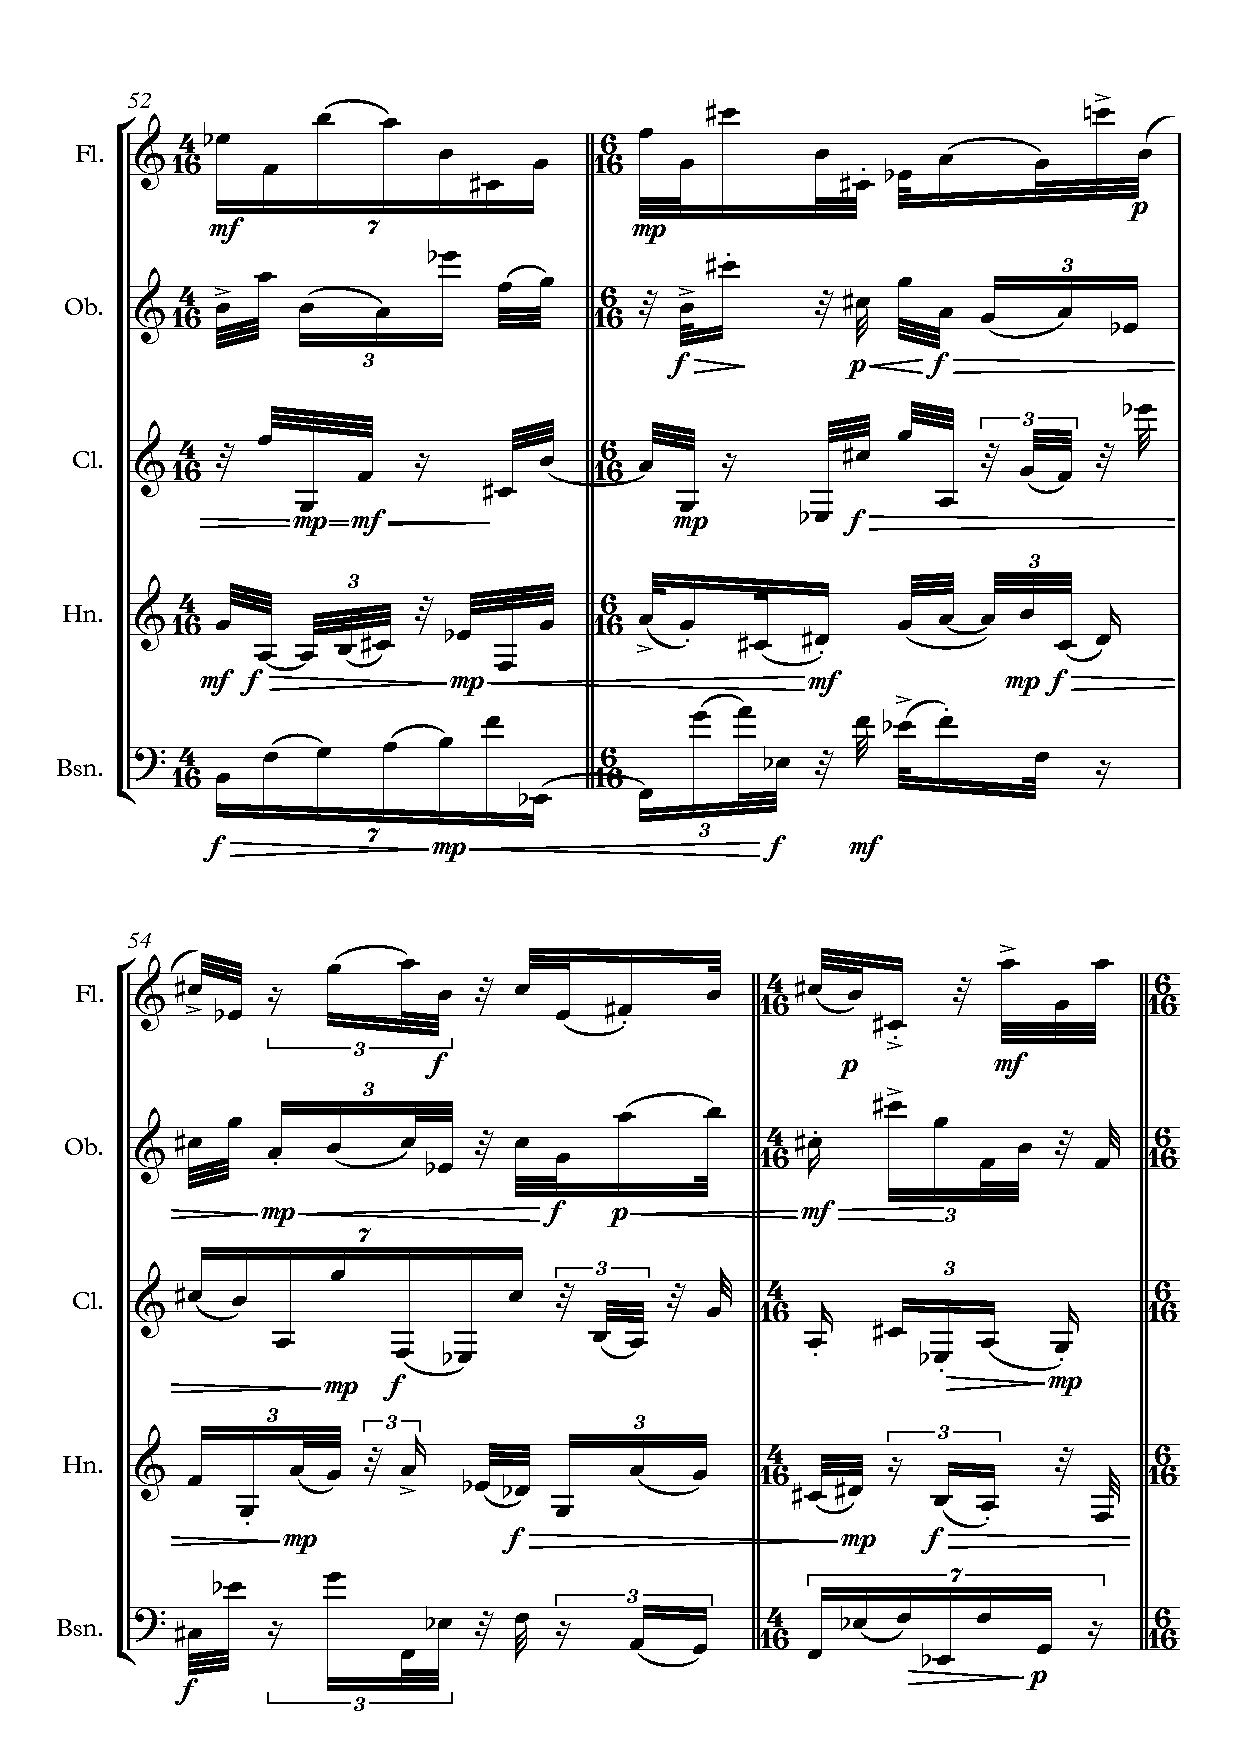
\includegraphics[width=6.5in]{figures/Out_of_Focus_11.pdf}
\end{figure}

%--------------------------------------------------------------------------
\begin{figure}[H]
    \centering
	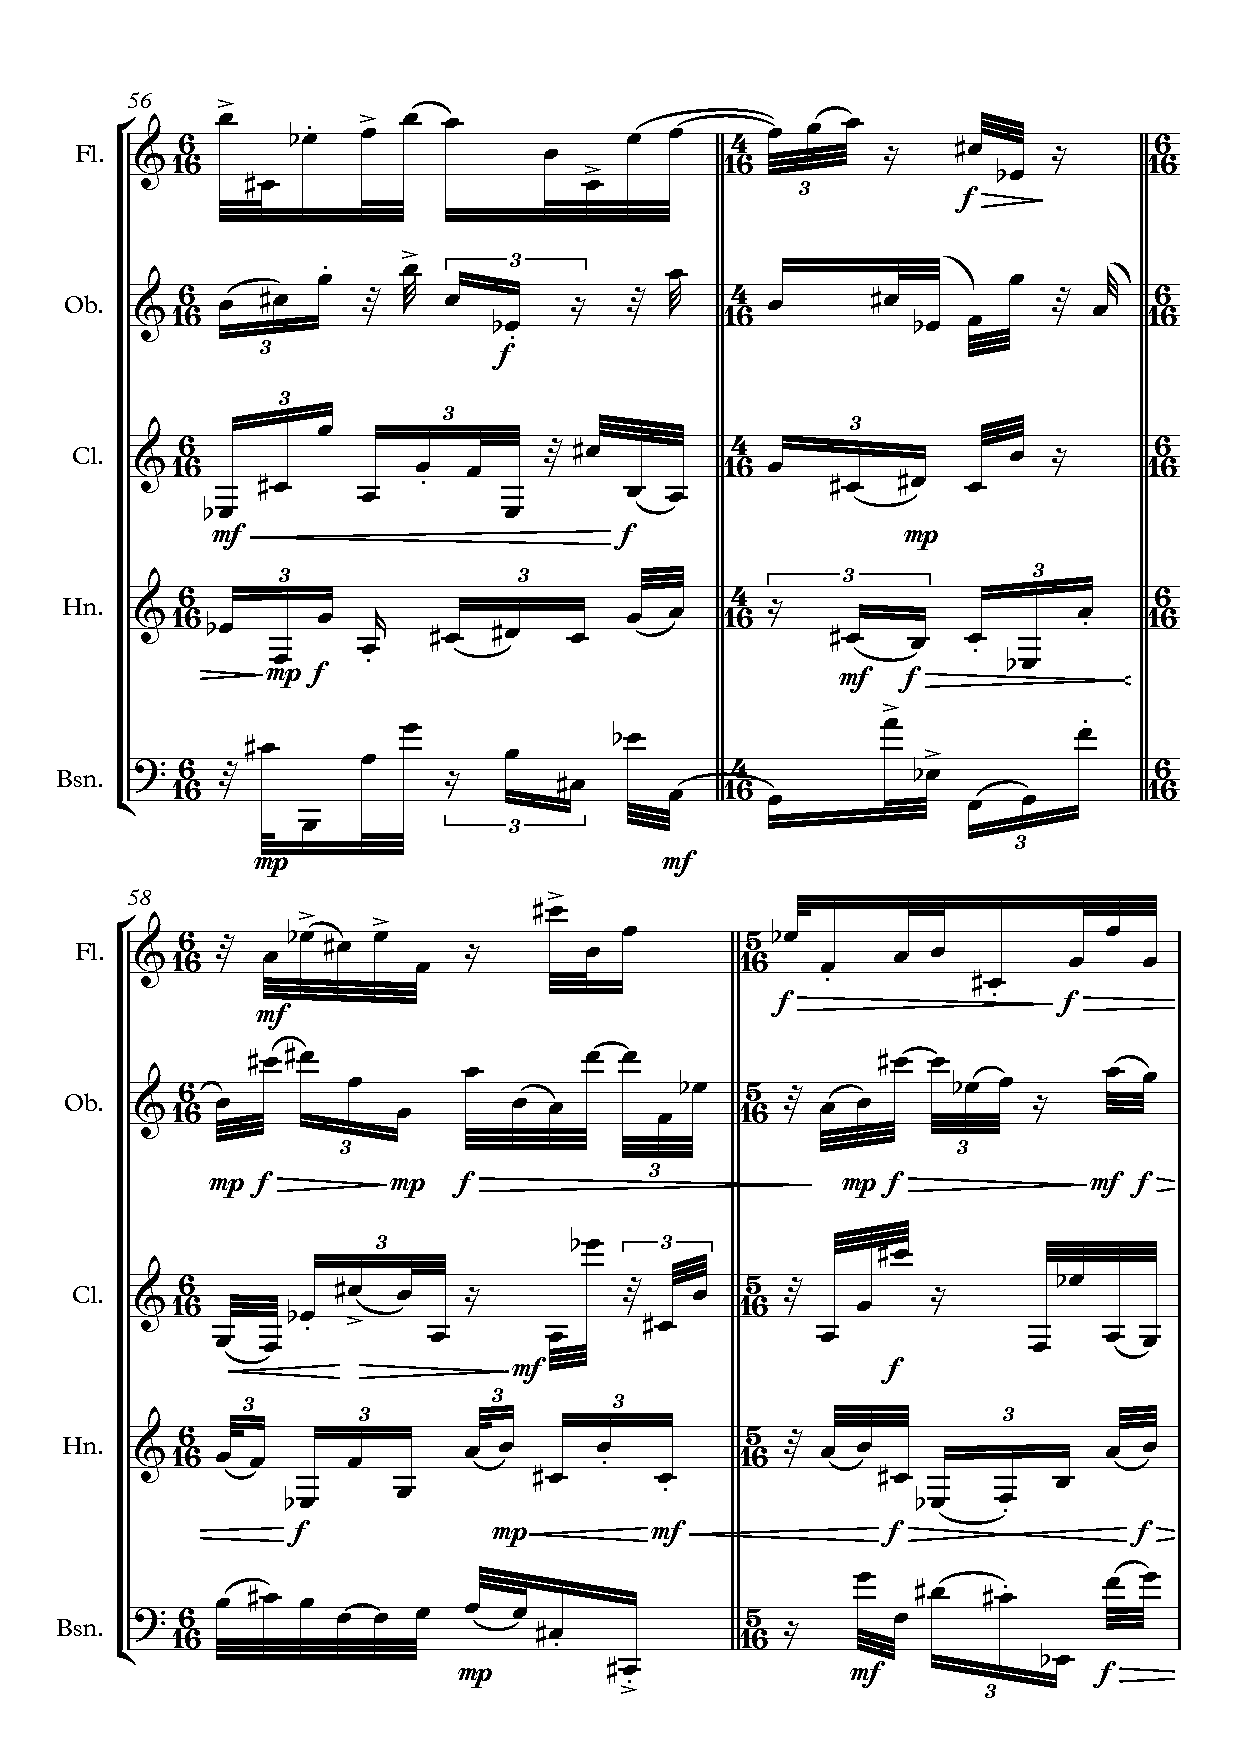
\includegraphics[width=6.5in]{figures/Out_of_Focus_12.pdf}
\end{figure}

%--------------------------------------------------------------------------
\begin{figure}[H]
    \centering
	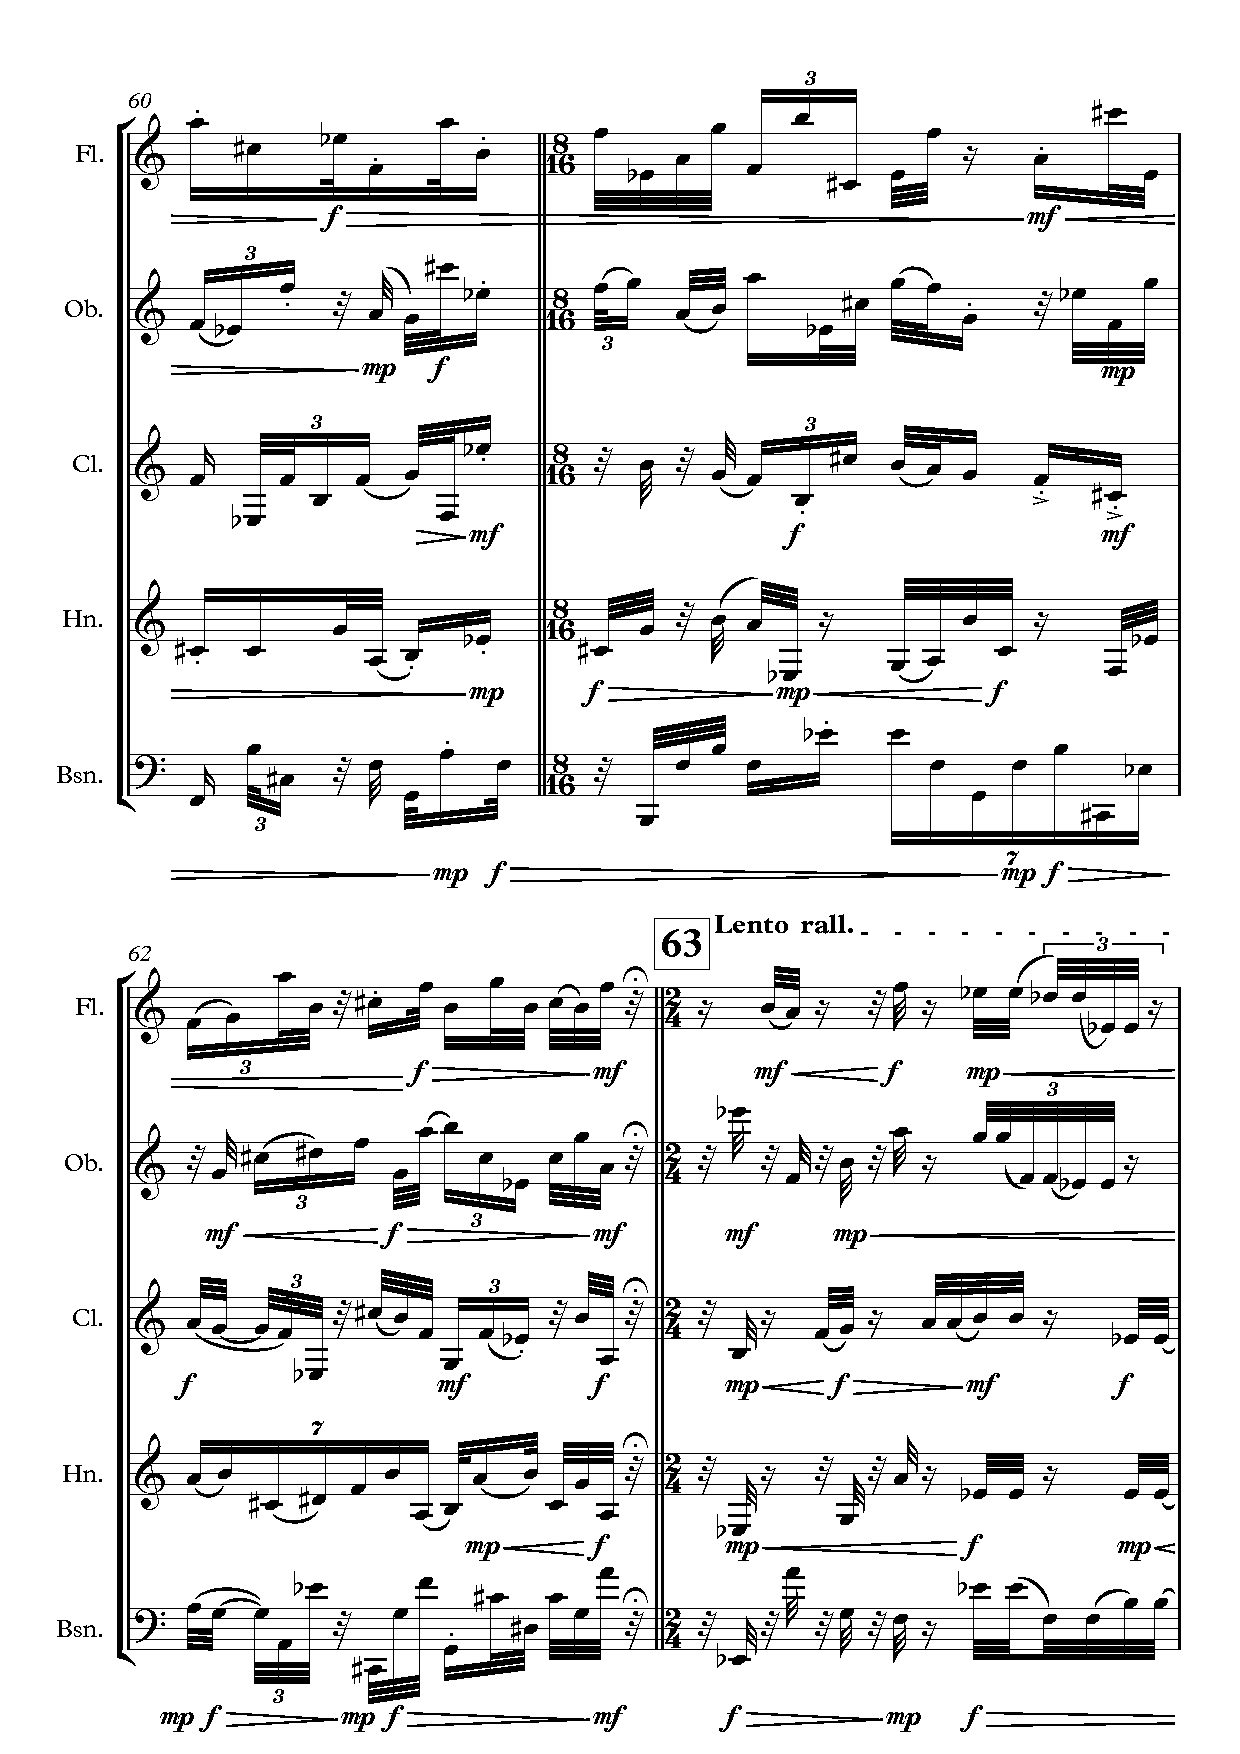
\includegraphics[width=6.5in]{figures/Out_of_Focus_13.pdf}
\end{figure}

%--------------------------------------------------------------------------
\begin{figure}[H]
    \centering
	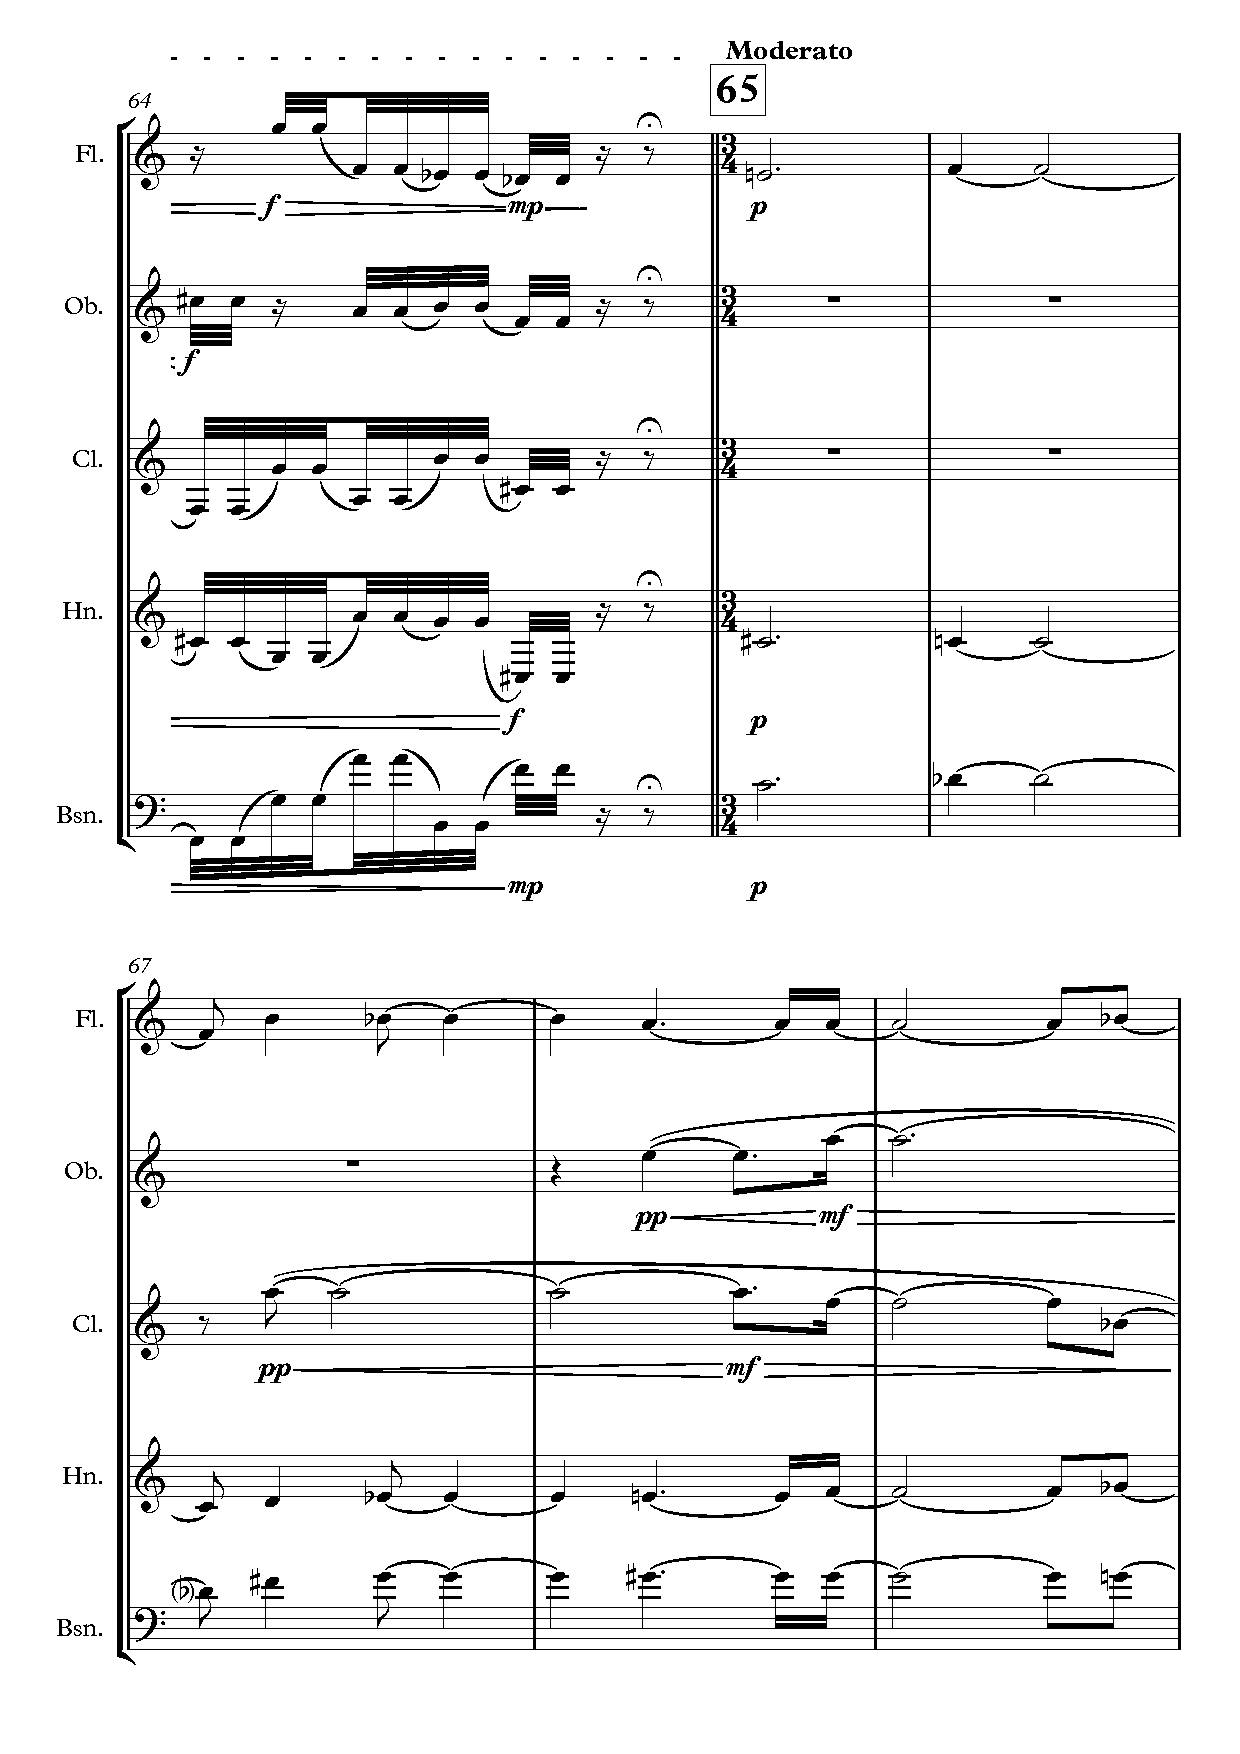
\includegraphics[width=6.5in]{figures/Out_of_Focus_14.pdf}
\end{figure}

%--------------------------------------------------------------------------
\begin{figure}[H]
    \centering
	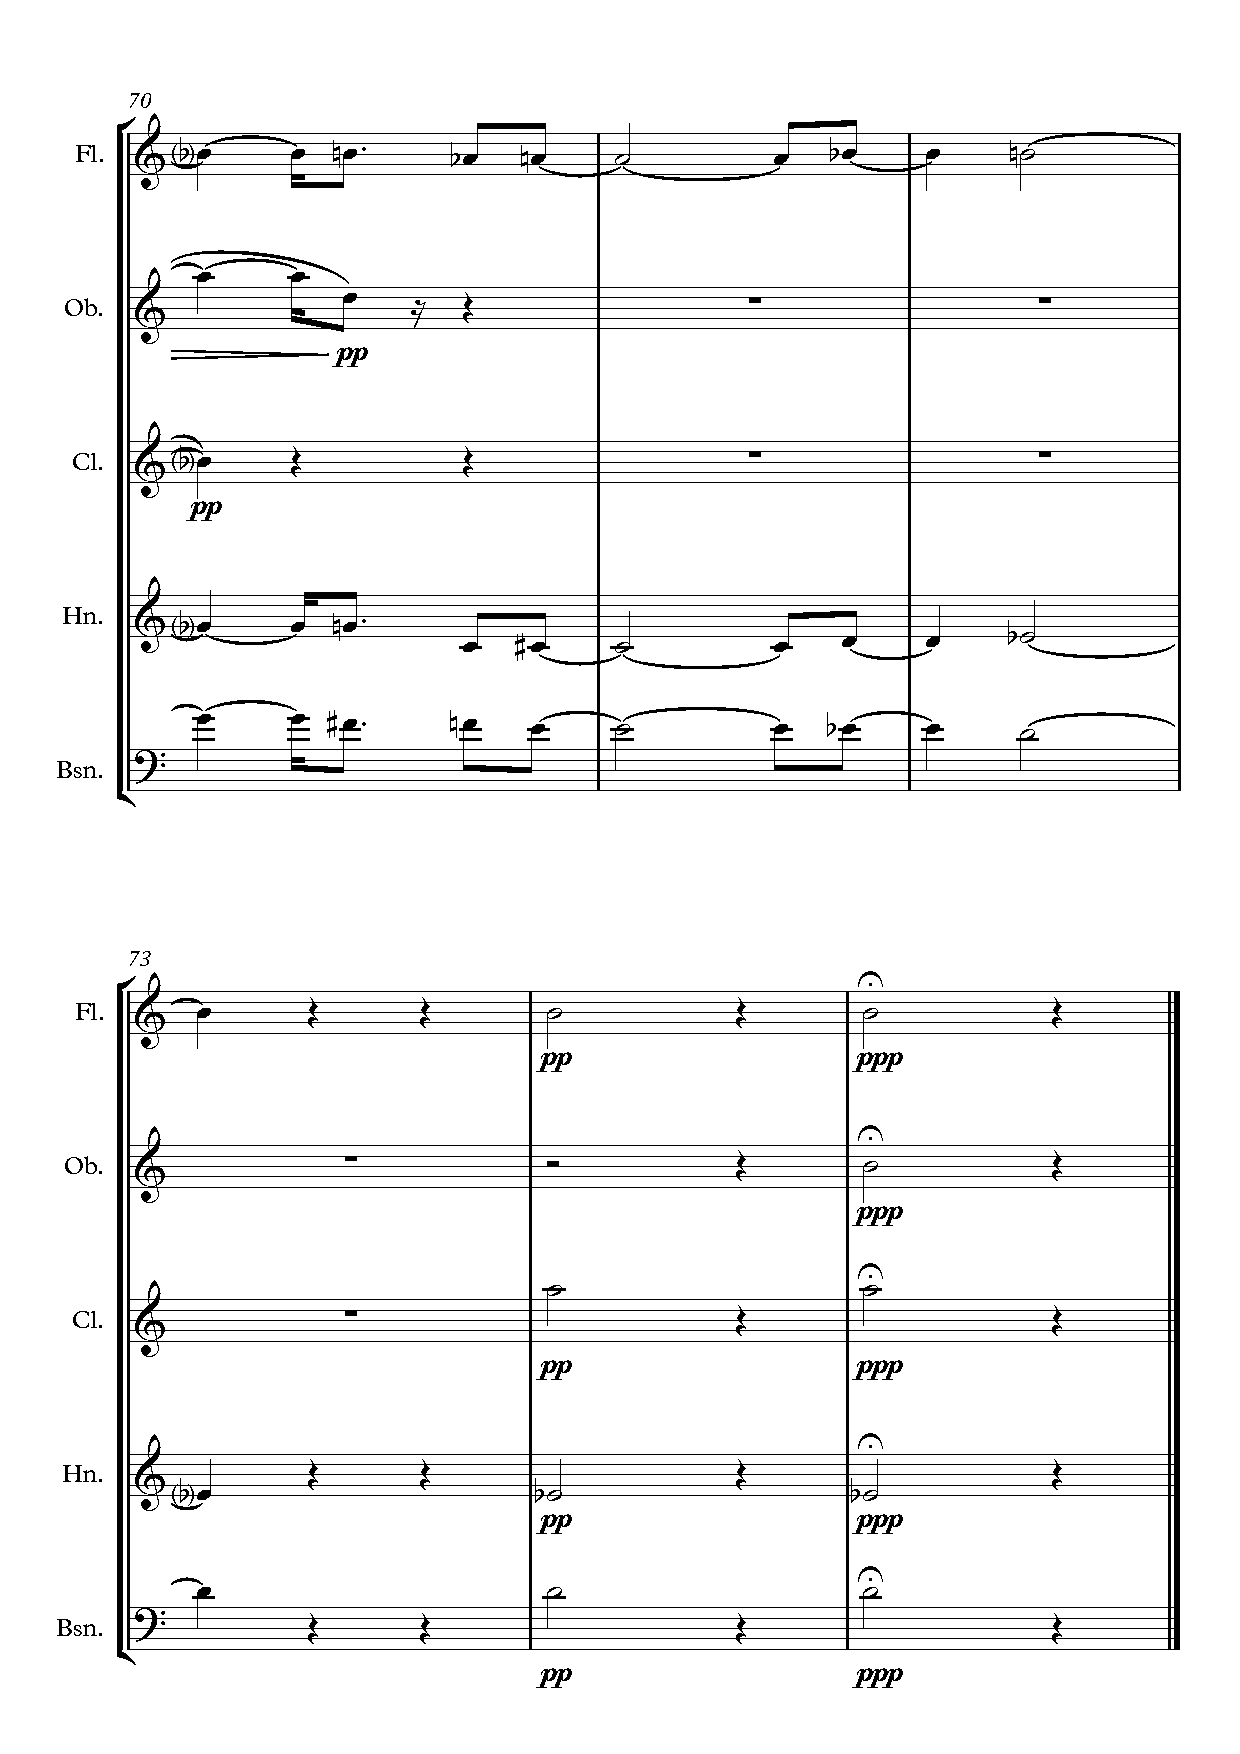
\includegraphics[width=6.5in]{figures/Out_of_Focus_15.pdf}
\end{figure}

%--------------------------------------------------------------------------
\section{Program Notes}

%--------------------------------------------------------------------------
\emph{Out of Focus for Wind Quintet} is a short piece in a single movement with three contrasting sections. The piece departs from a generative algorithm which is stochastic in nature. Every instrument is centered around a particular note, and the algorithm dictates how these central notes evolve in terms of pitch and octave displacements, dynamics, and durations. The raw output of the algorithm is brought to life in a second and final compositional stage, where a myriad of adjustments and gestures are added to make the instruments sing. \emph{Out of Focus} was composed in 2014 and premiered as part of the Society of Composers, Inc. Showcase. The event took place at the University of Florida on February 7\textsuperscript{th} of 2015.

%--------------------------------------------------------------------------
\chapter{Duo for Alto Saxophone and Viola}

%--------------------------------------------------------------------------
\begin{figure}[h!]
    \centering
	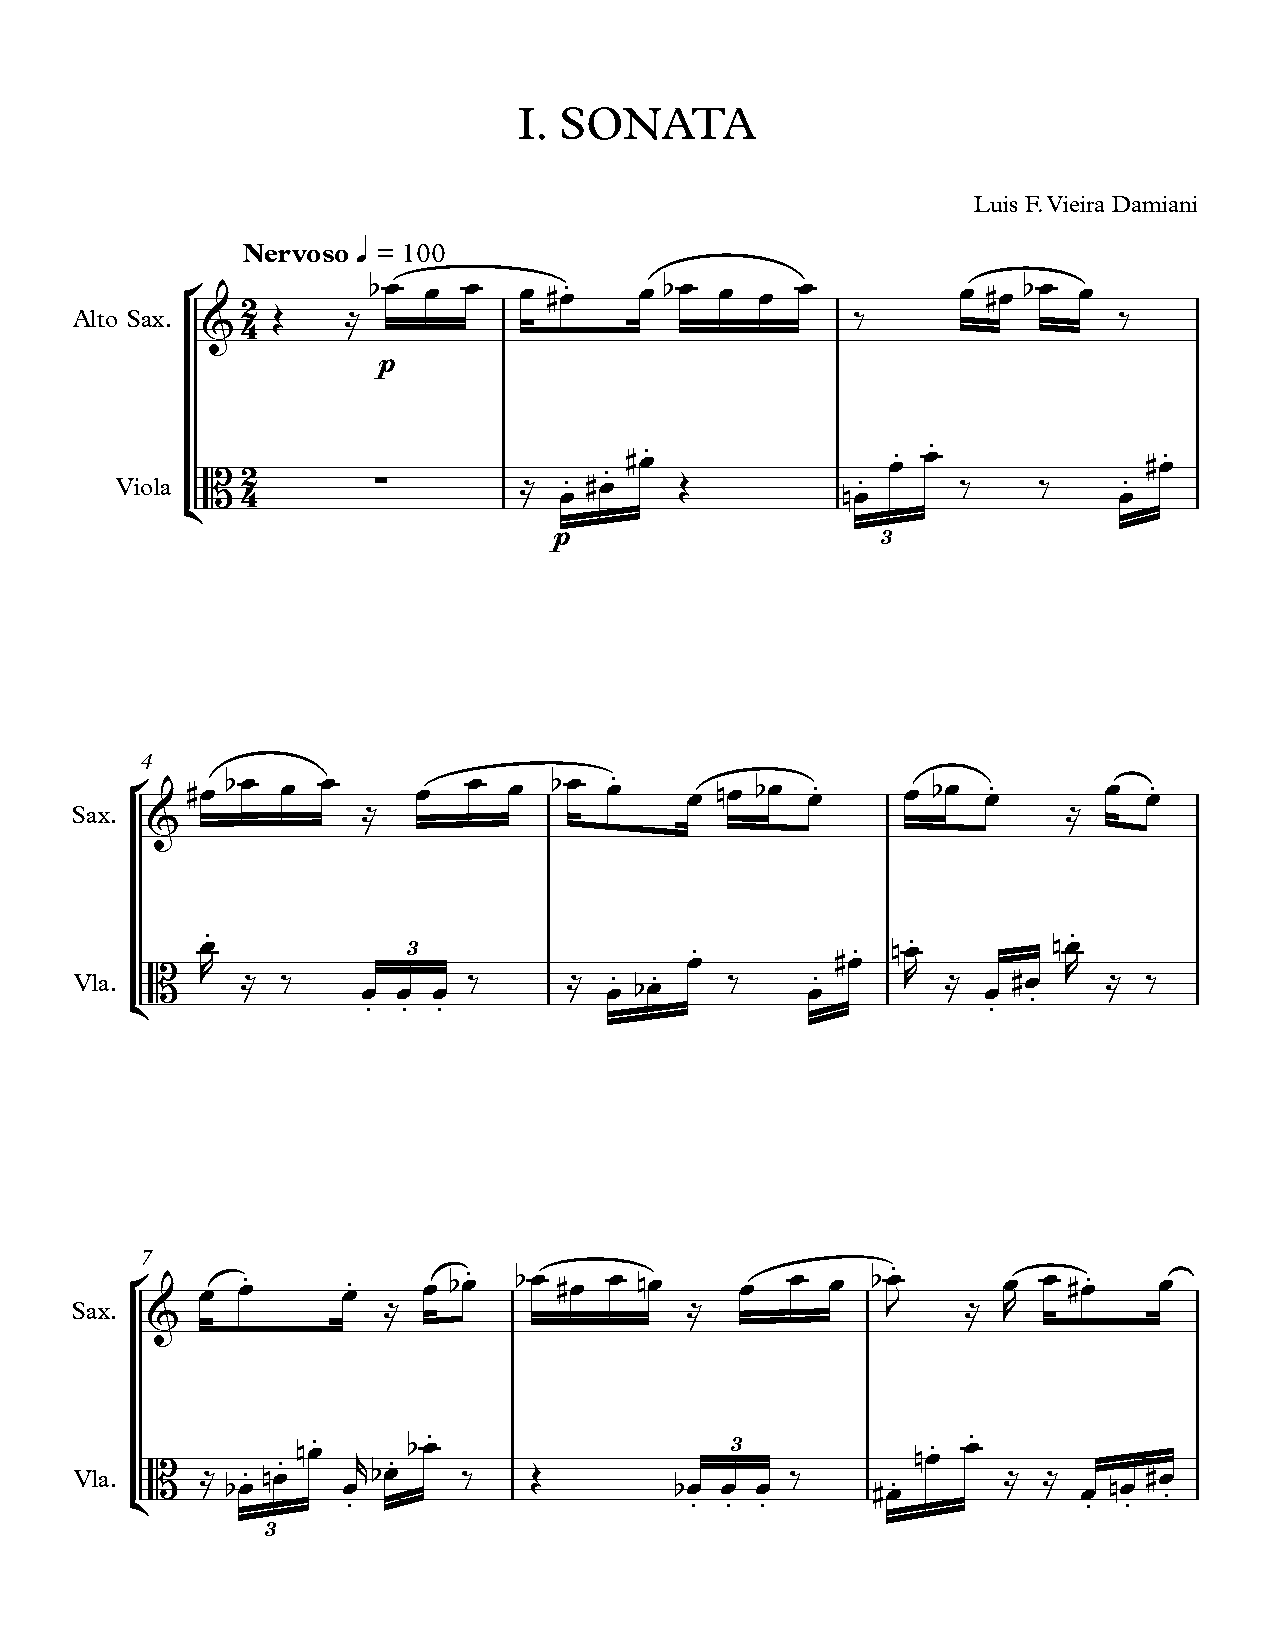
\includegraphics[width=6.5in]{figures/Sax_Viola_1.pdf}
\end{figure}

%--------------------------------------------------------------------------
\begin{figure}[htbp]
    \centering
	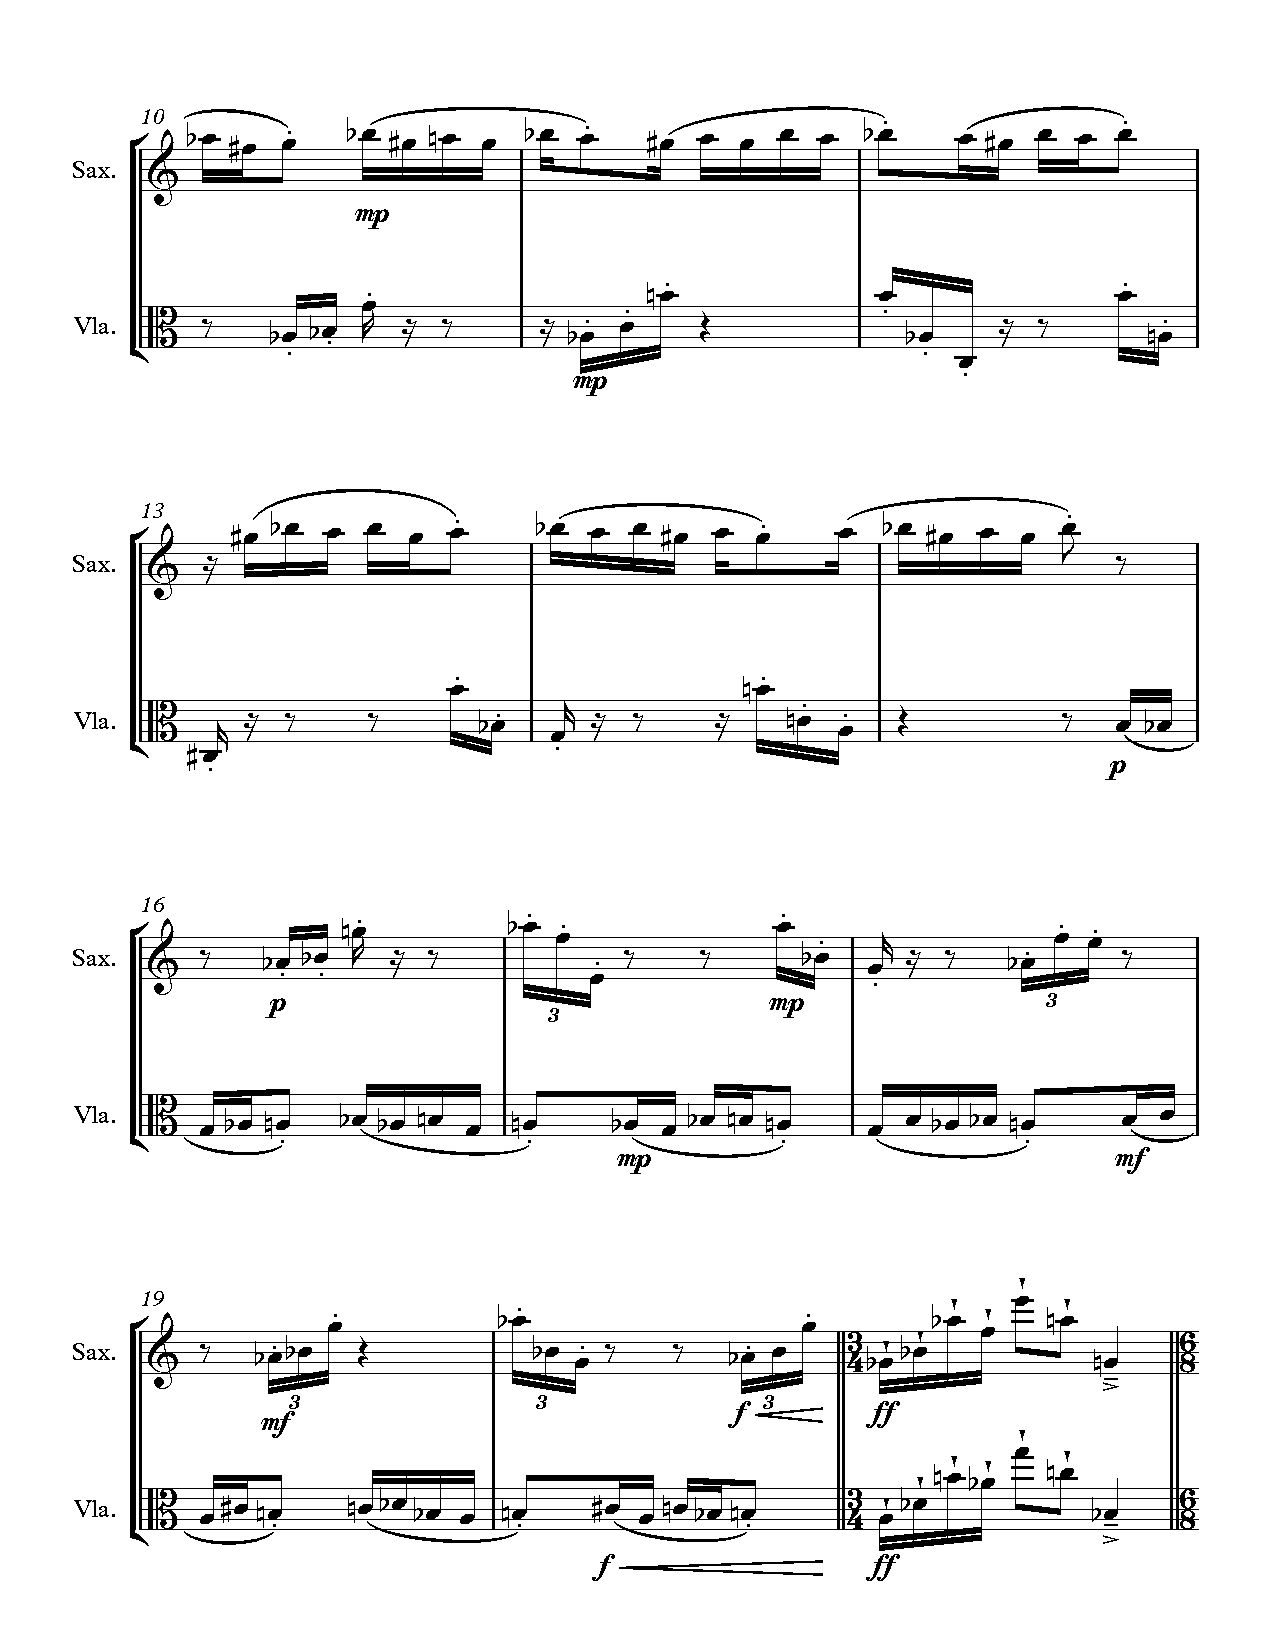
\includegraphics[width=6.5in]{figures/Sax_Viola_2.pdf}
\end{figure}

%--------------------------------------------------------------------------
\begin{figure}[htbp]
    \centering
	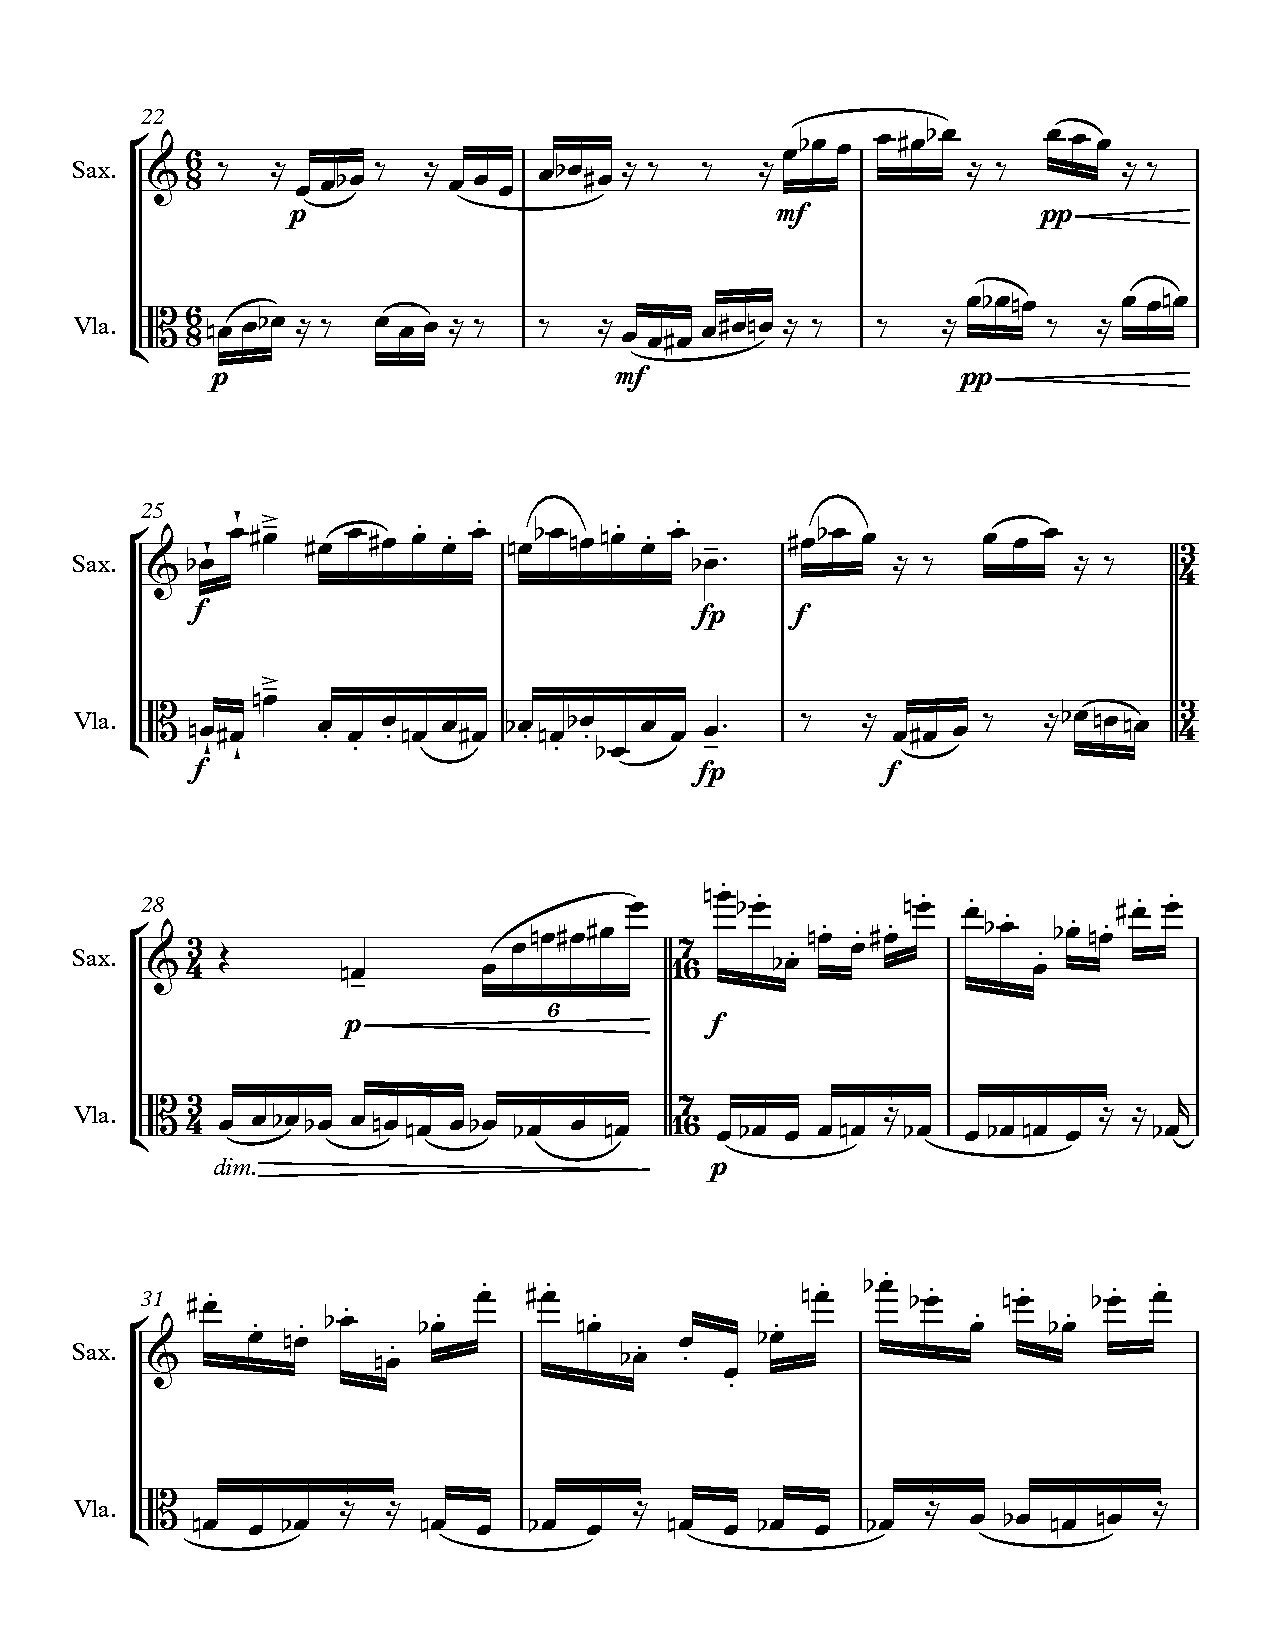
\includegraphics[width=6.5in]{figures/Sax_Viola_3.pdf}
\end{figure}

%--------------------------------------------------------------------------
\begin{figure}[htbp]
    \centering
	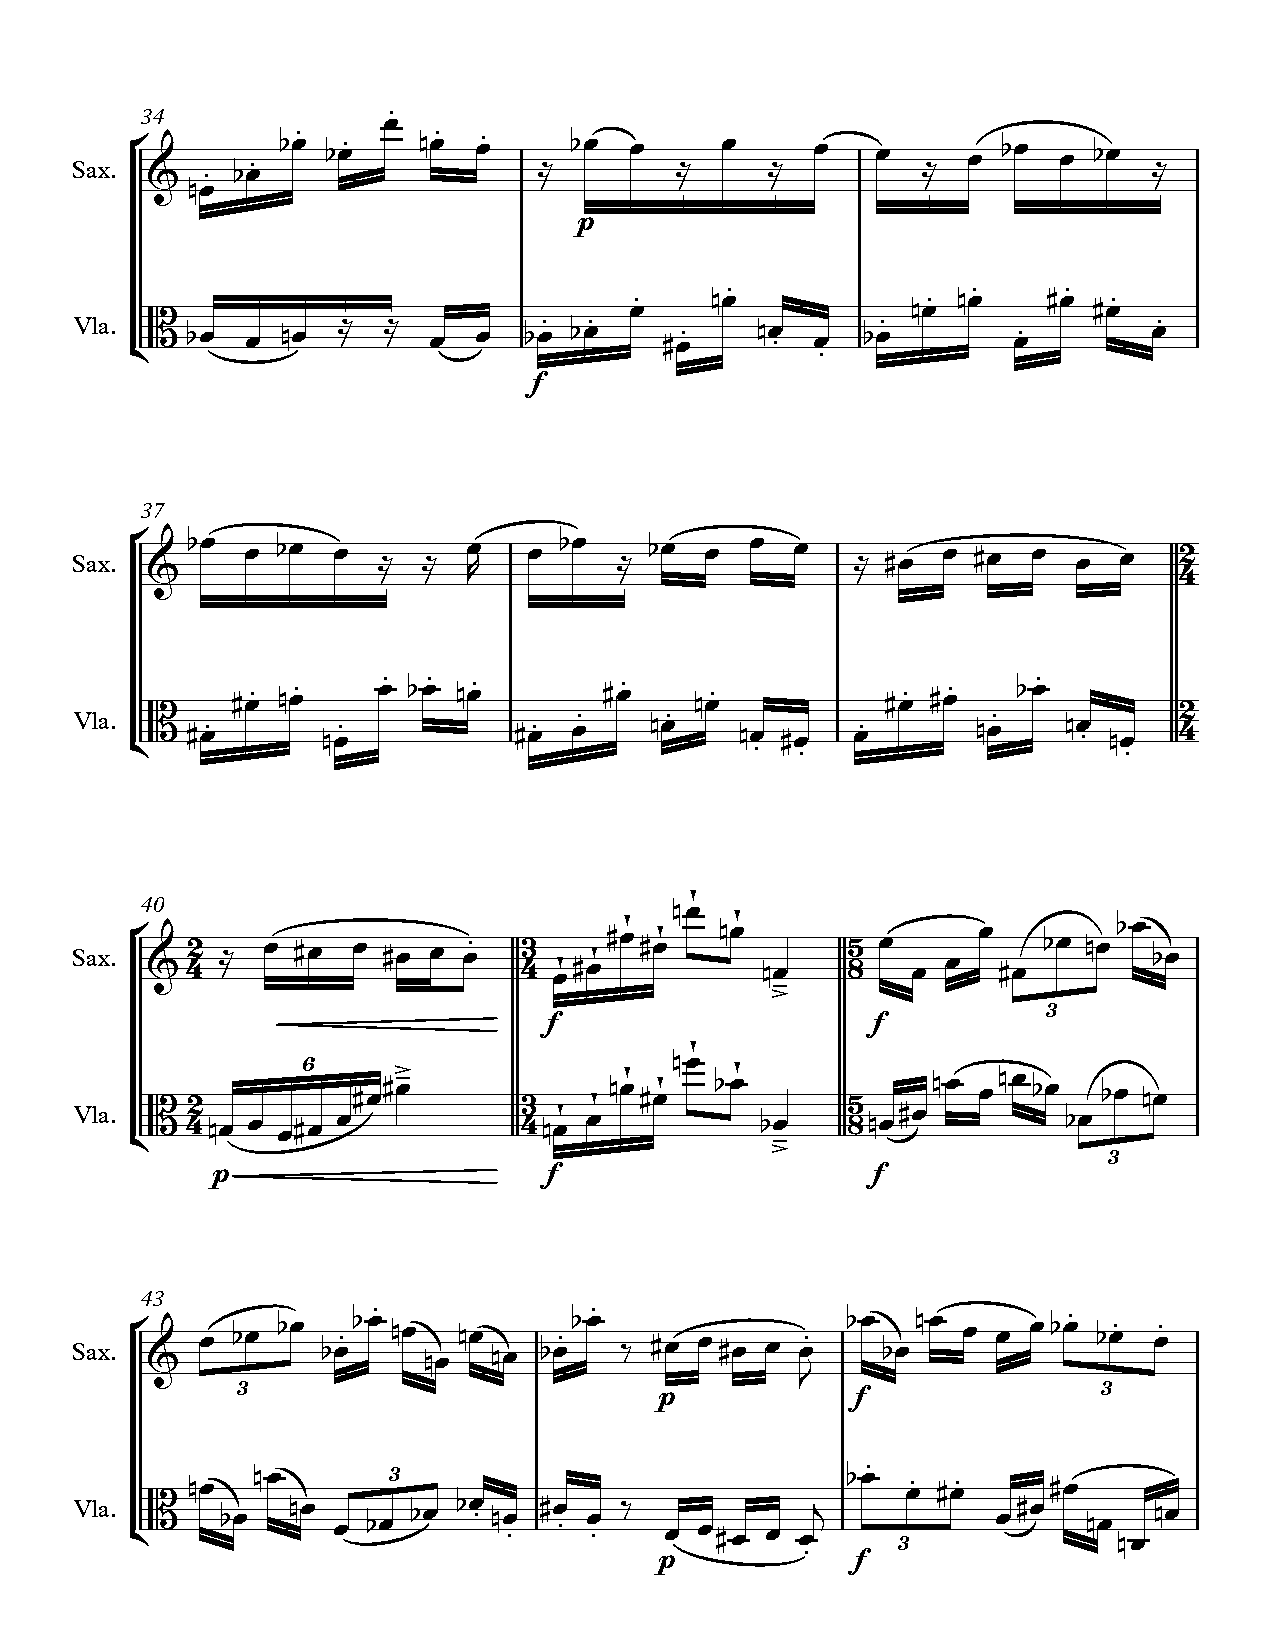
\includegraphics[width=6.5in]{figures/Sax_Viola_4.pdf}
\end{figure}

%--------------------------------------------------------------------------
\begin{figure}[htbp]
    \centering
	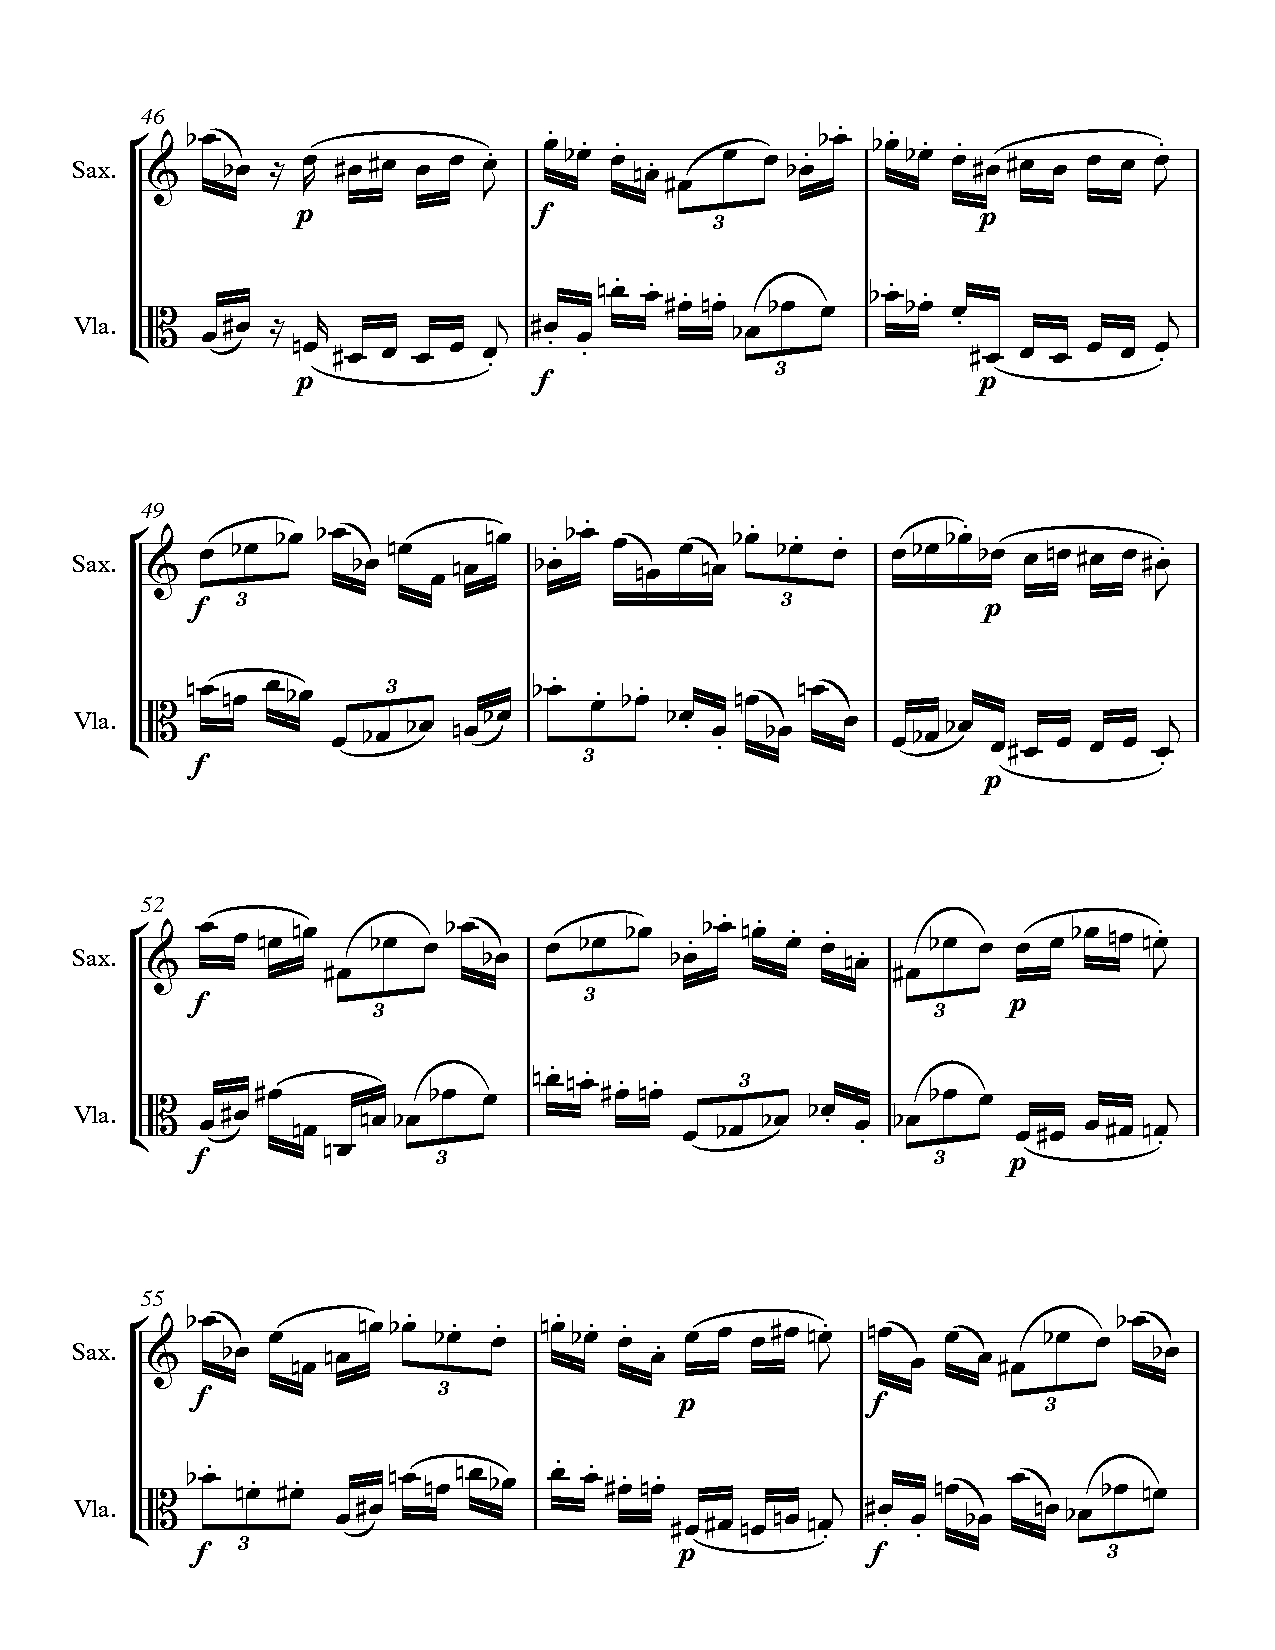
\includegraphics[width=6.5in]{figures/Sax_Viola_5.pdf}
\end{figure}

%--------------------------------------------------------------------------
\begin{figure}[htbp]
    \centering
	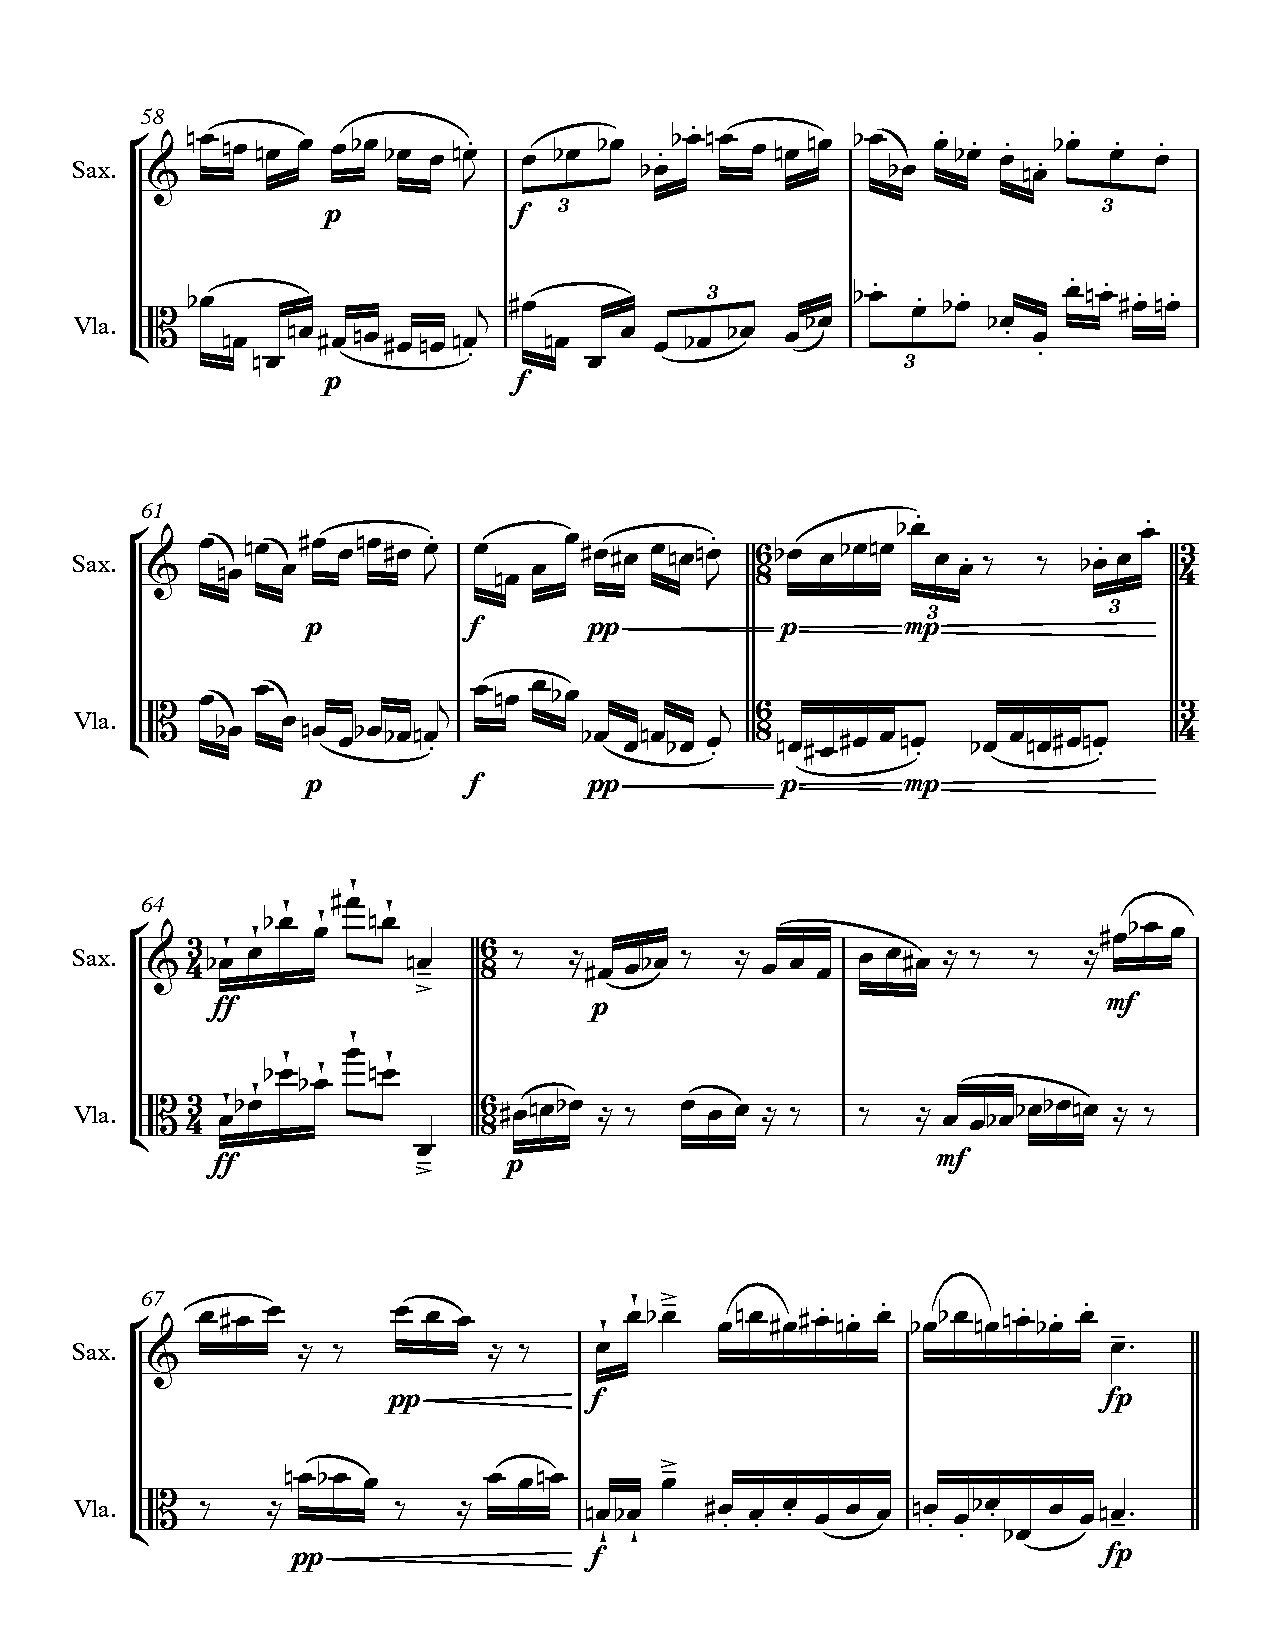
\includegraphics[width=6.5in]{figures/Sax_Viola_6.pdf}
\end{figure}

%--------------------------------------------------------------------------
\begin{figure}[htbp]
    \centering
	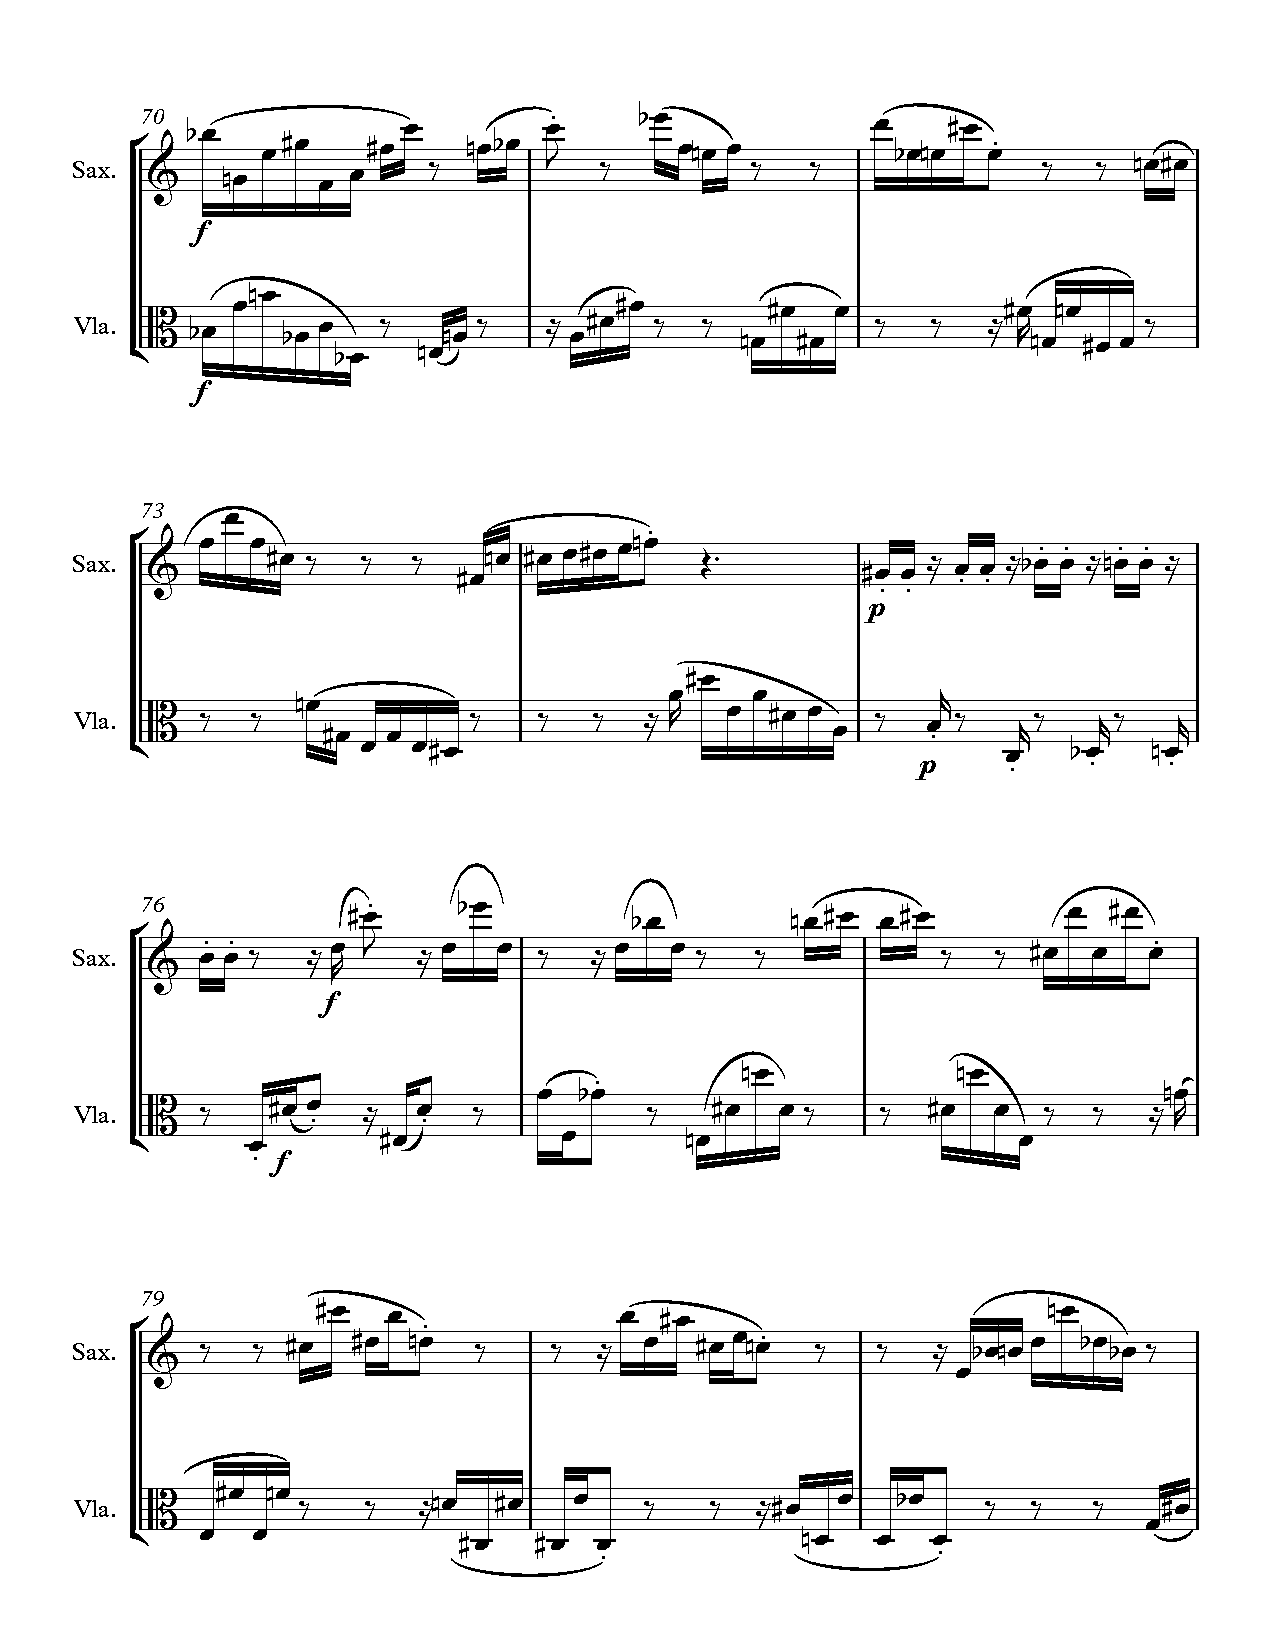
\includegraphics[width=6.5in]{figures/Sax_Viola_7.pdf}
\end{figure}

%--------------------------------------------------------------------------
\begin{figure}[htbp]
    \centering
	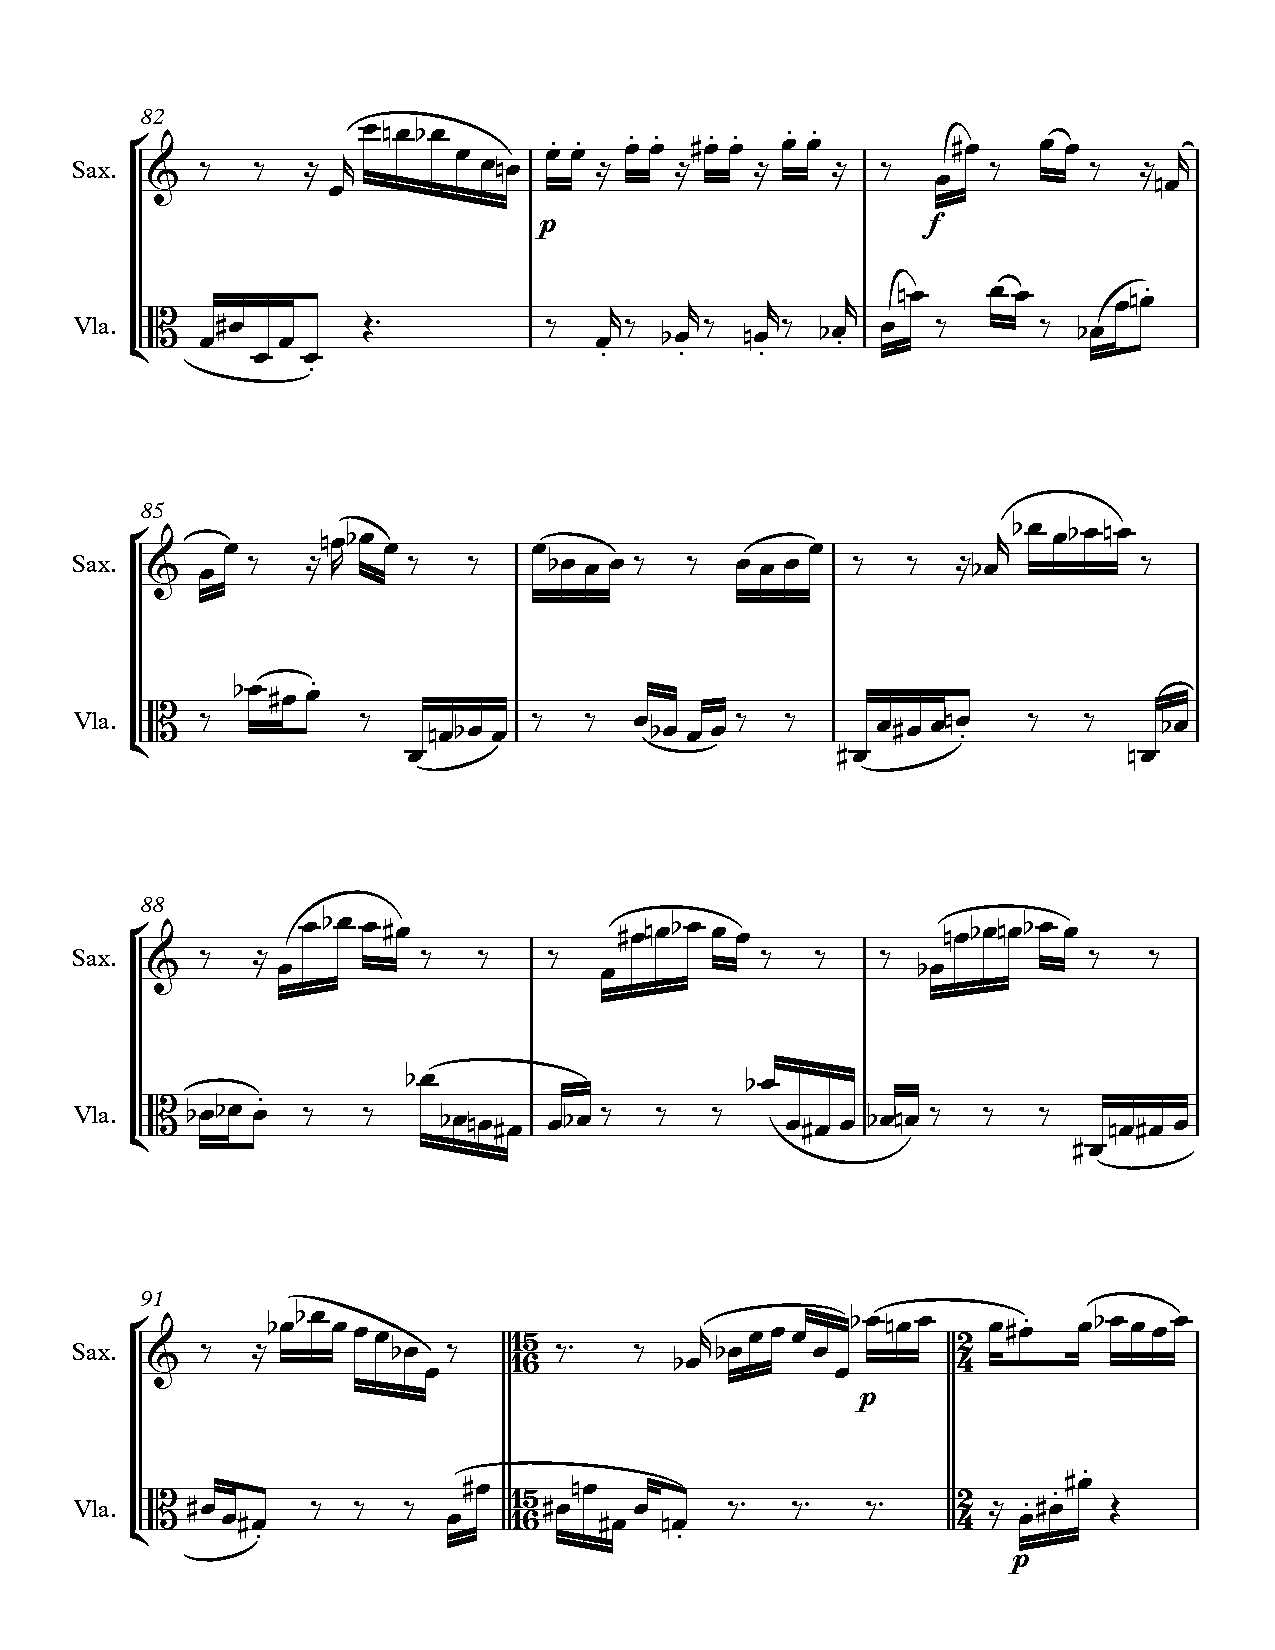
\includegraphics[width=6.5in]{figures/Sax_Viola_8.pdf}
\end{figure}

%--------------------------------------------------------------------------
\begin{figure}[htbp]
    \centering
	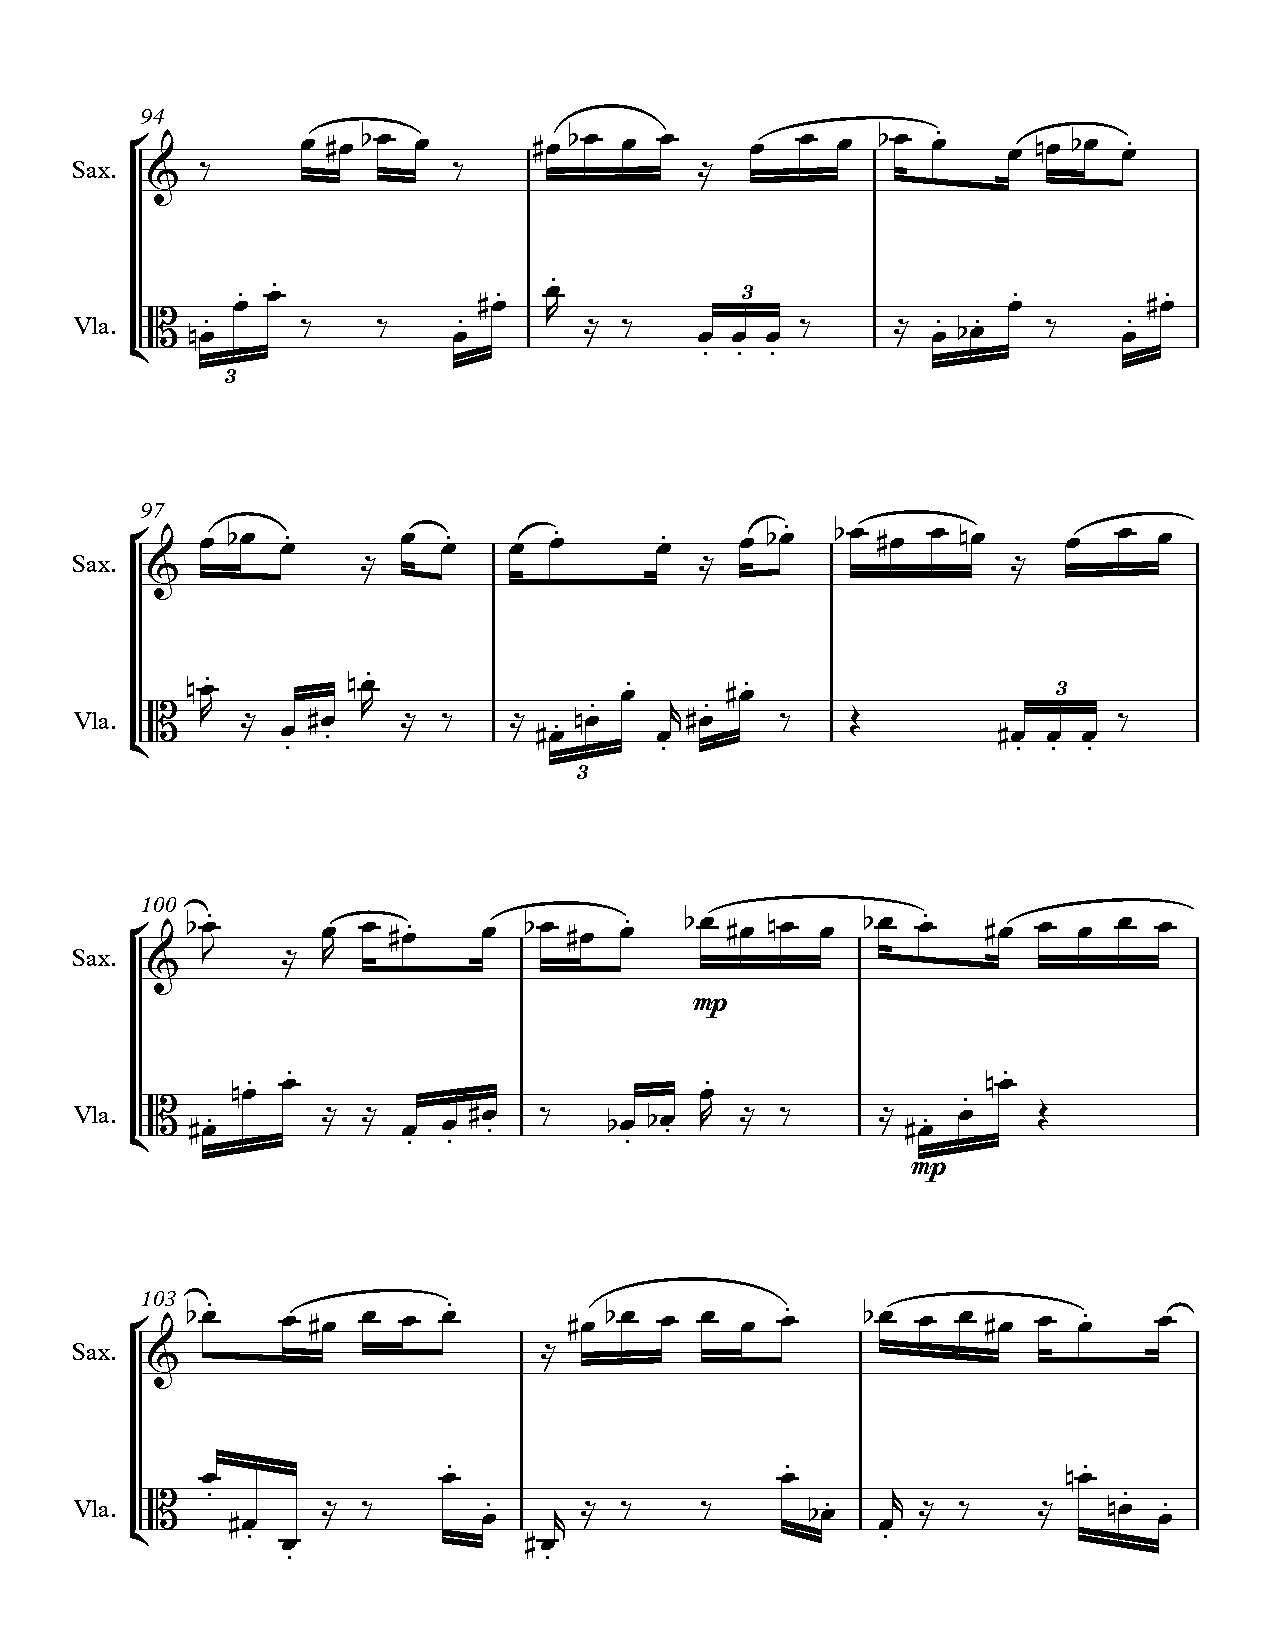
\includegraphics[width=6.5in]{figures/Sax_Viola_9.pdf}
\end{figure}

%--------------------------------------------------------------------------
\begin{figure}[htbp]
    \centering
	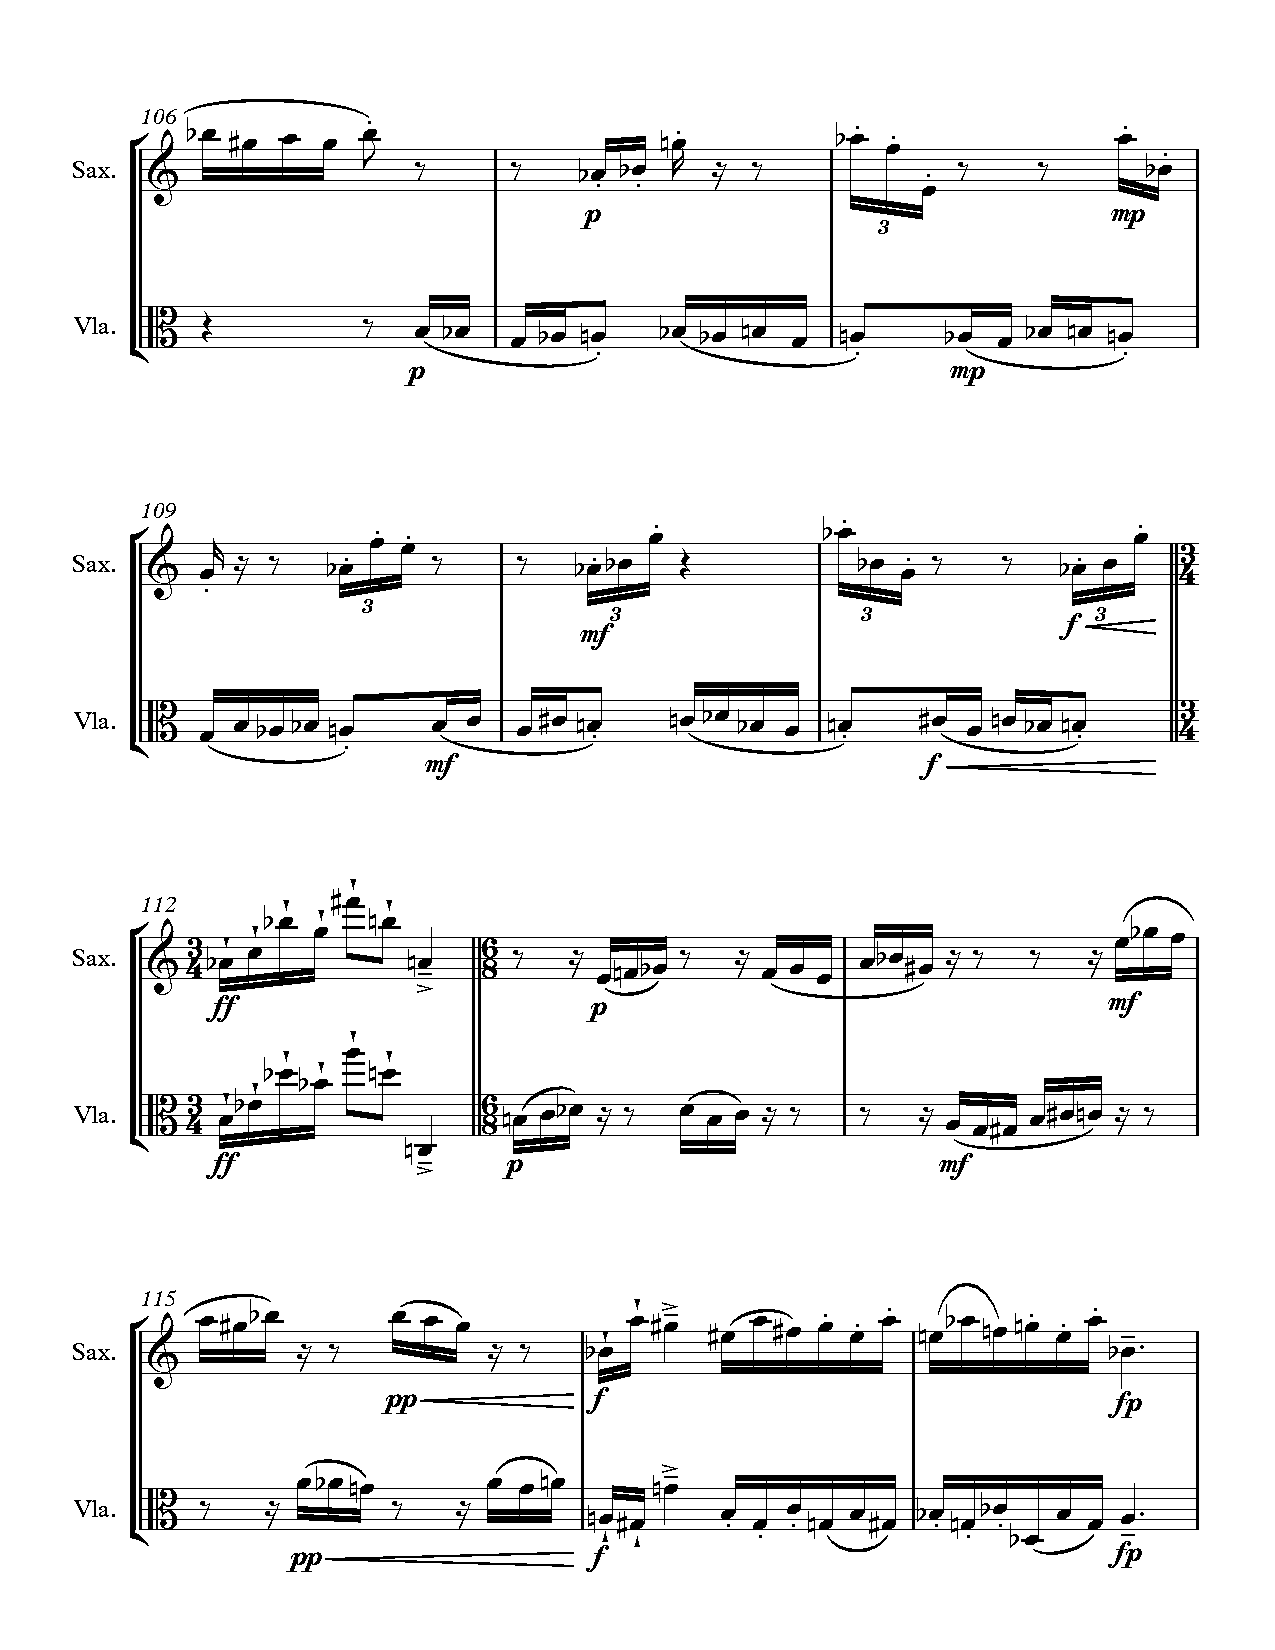
\includegraphics[width=6.5in]{figures/Sax_Viola_10.pdf}
\end{figure}

%--------------------------------------------------------------------------
\begin{figure}[htbp]
    \centering
	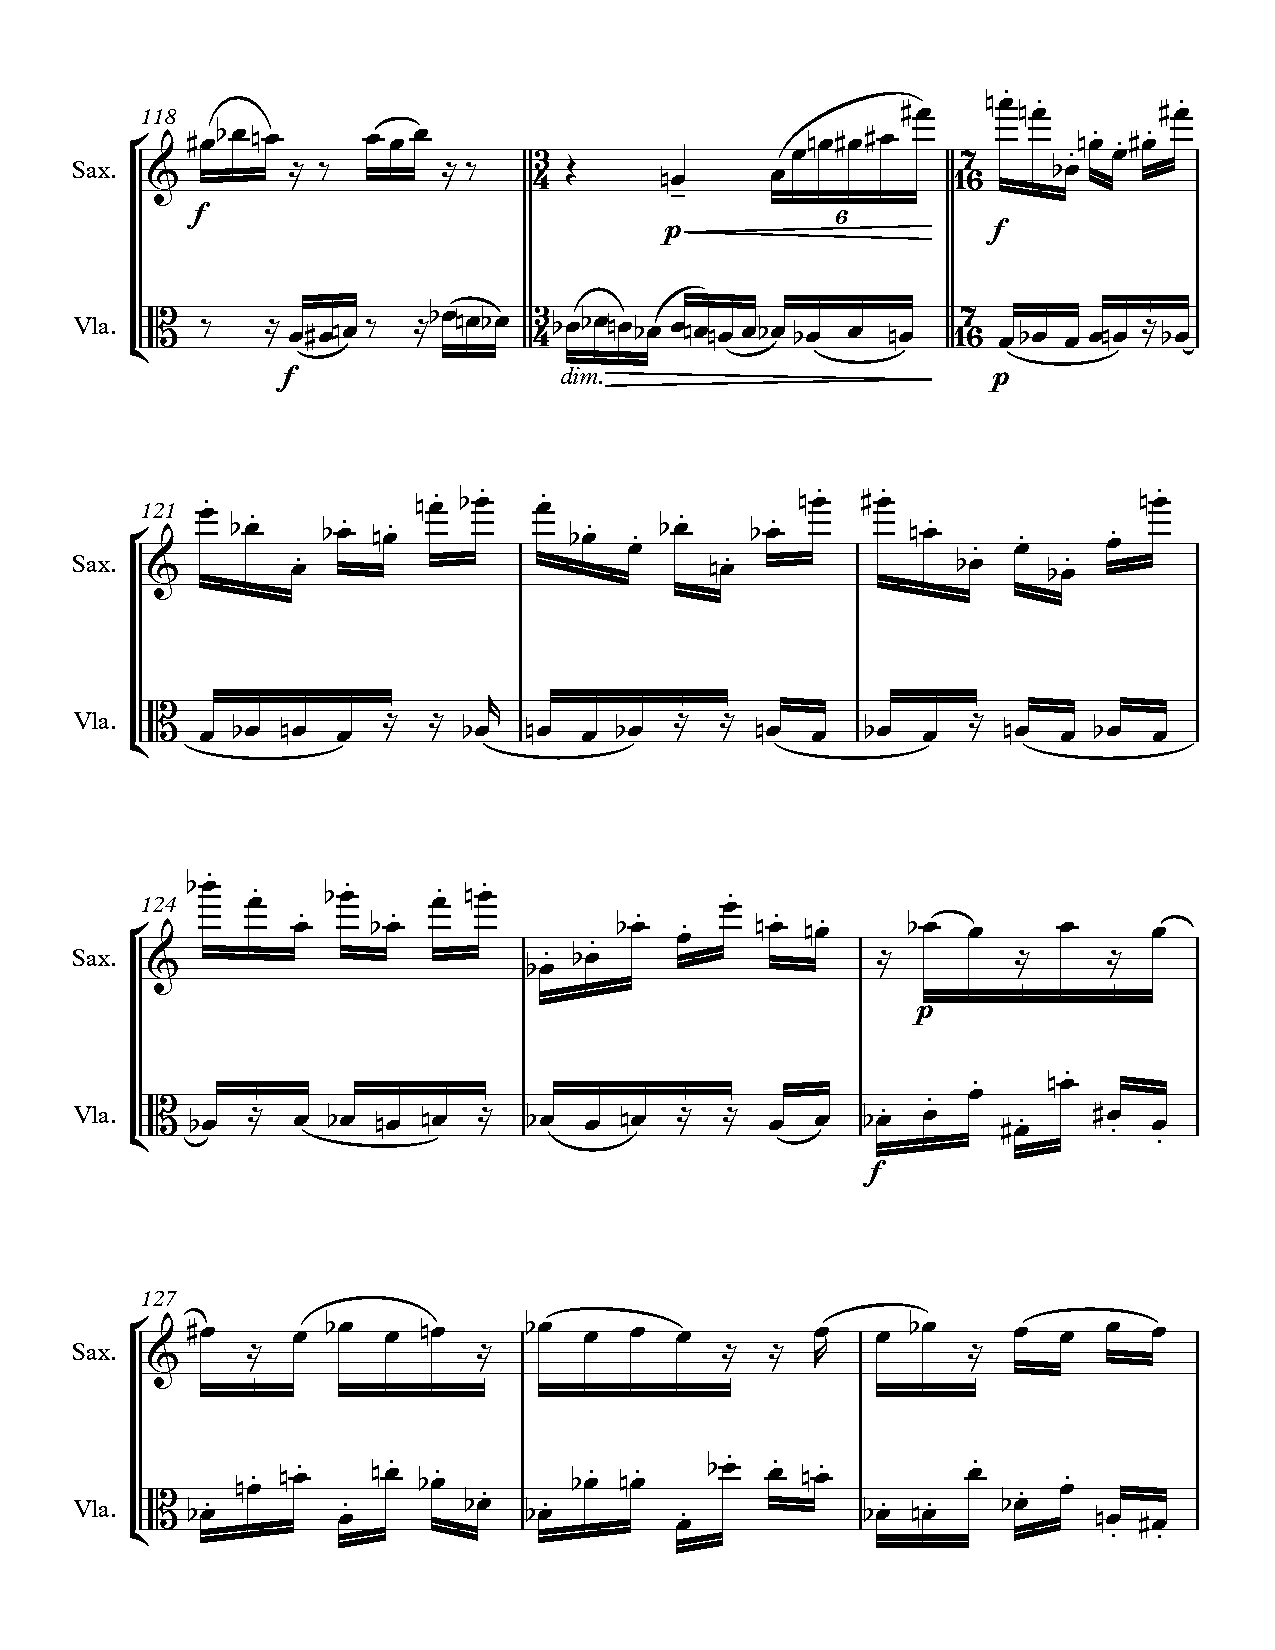
\includegraphics[width=6.5in]{figures/Sax_Viola_11.pdf}
\end{figure}

%--------------------------------------------------------------------------
\begin{figure}[htbp]
    \centering
	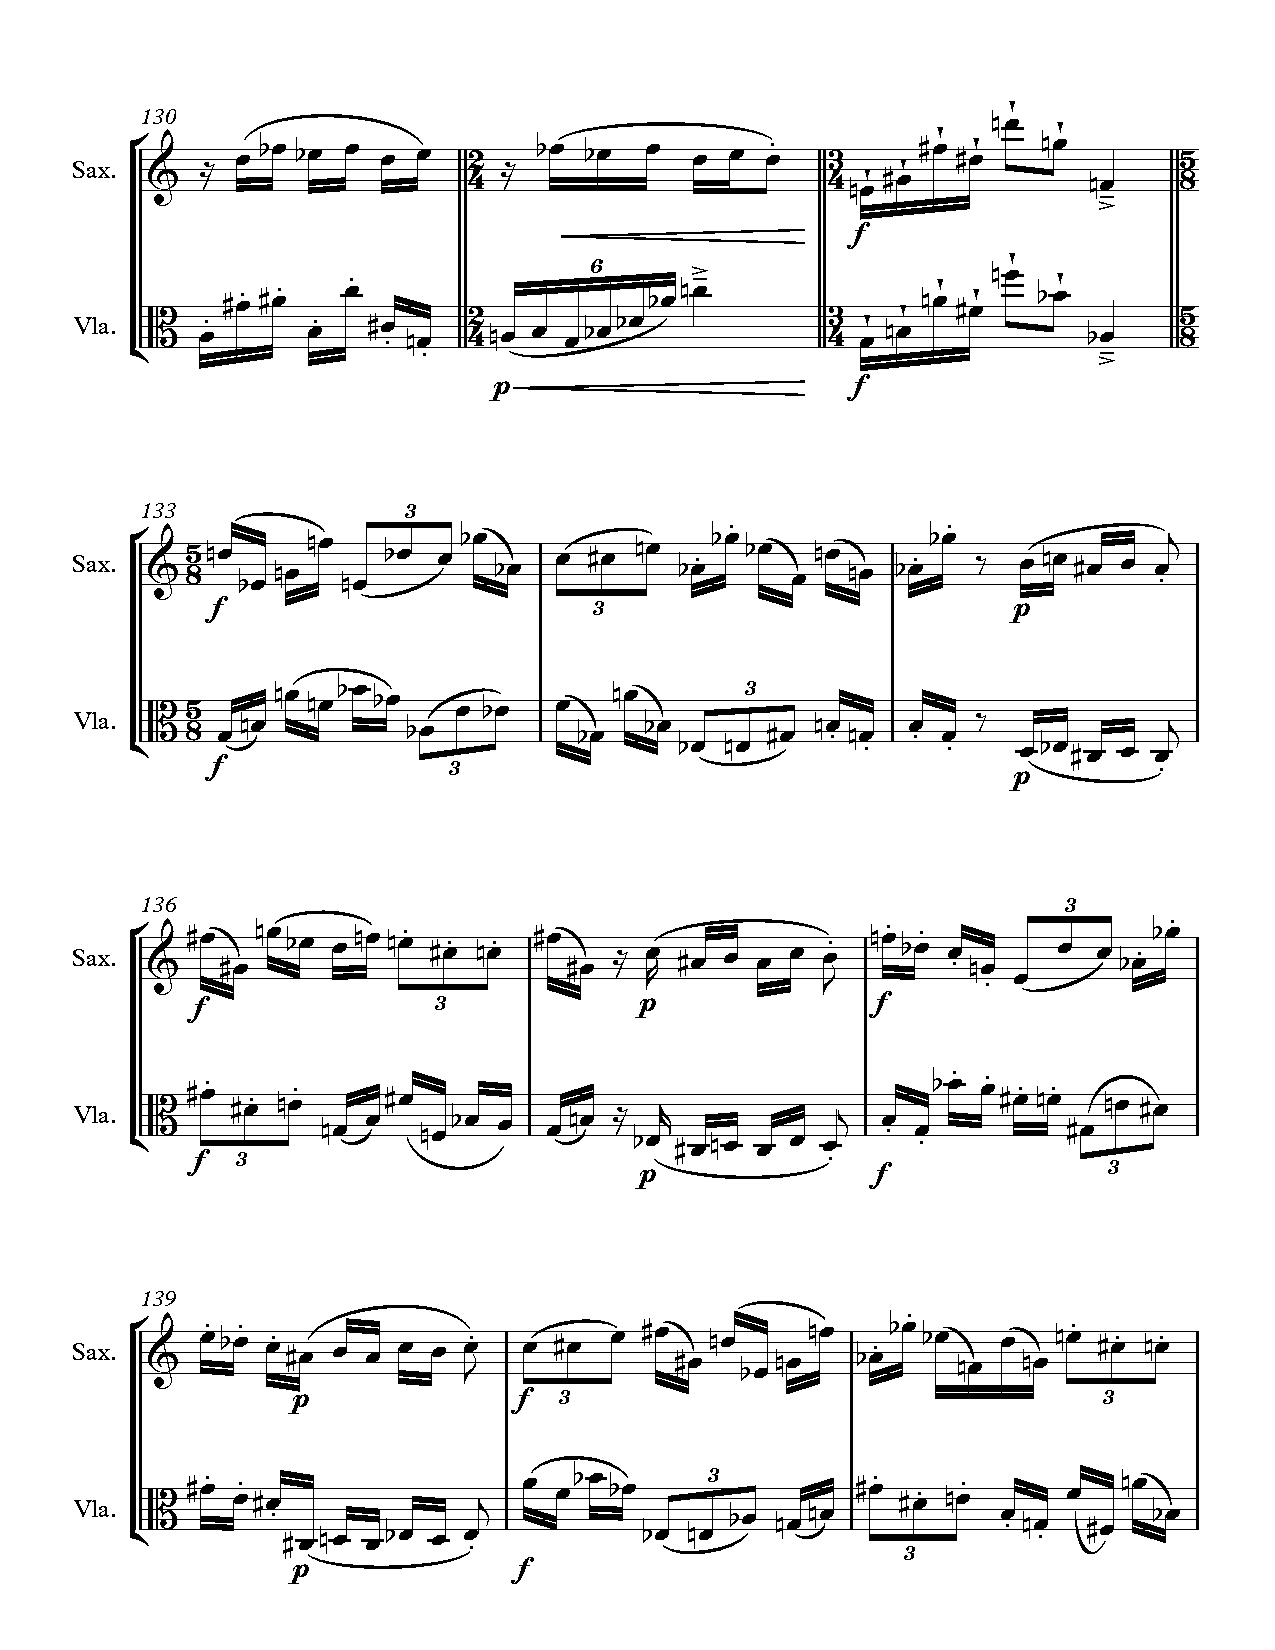
\includegraphics[width=6.5in]{figures/Sax_Viola_12.pdf}
\end{figure}

%--------------------------------------------------------------------------
\begin{figure}[htbp]
    \centering
	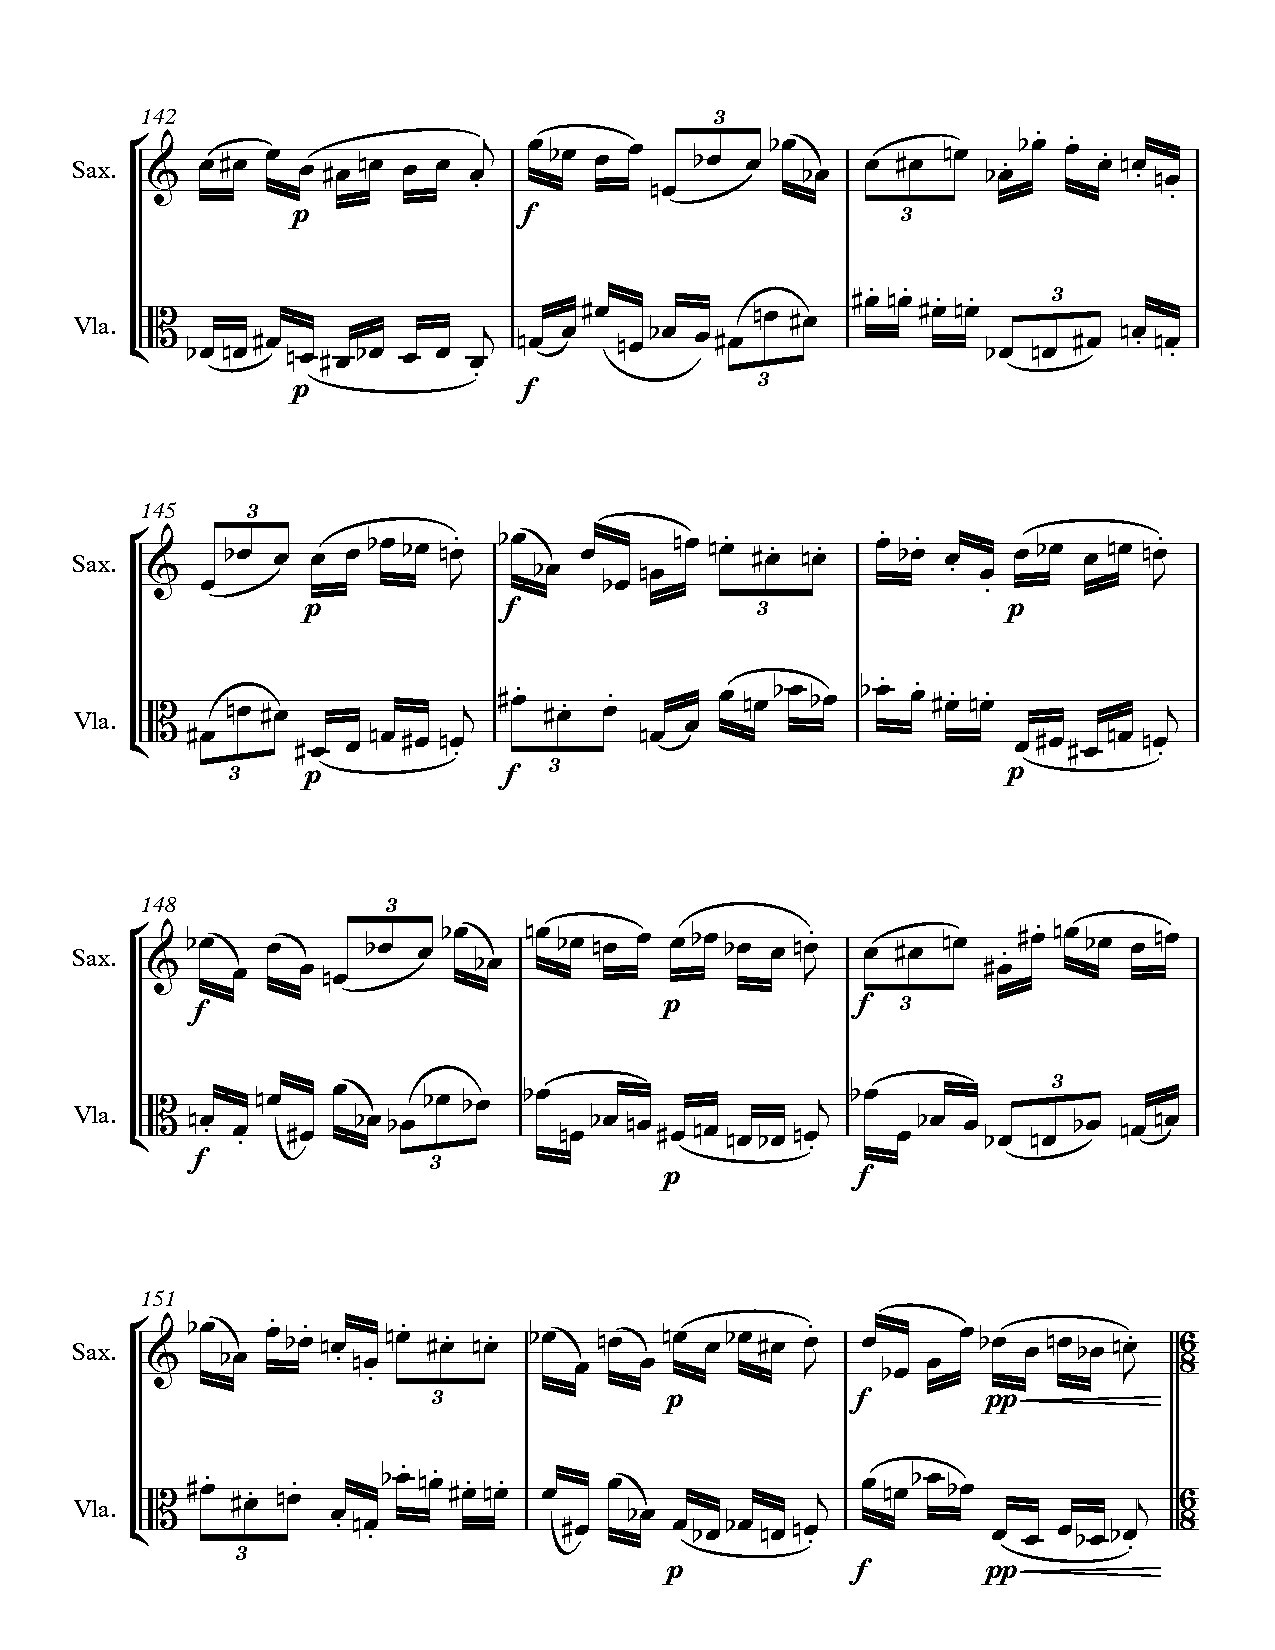
\includegraphics[width=6.5in]{figures/Sax_Viola_13.pdf}
\end{figure}

%--------------------------------------------------------------------------
\begin{figure}[htbp]
    \centering
	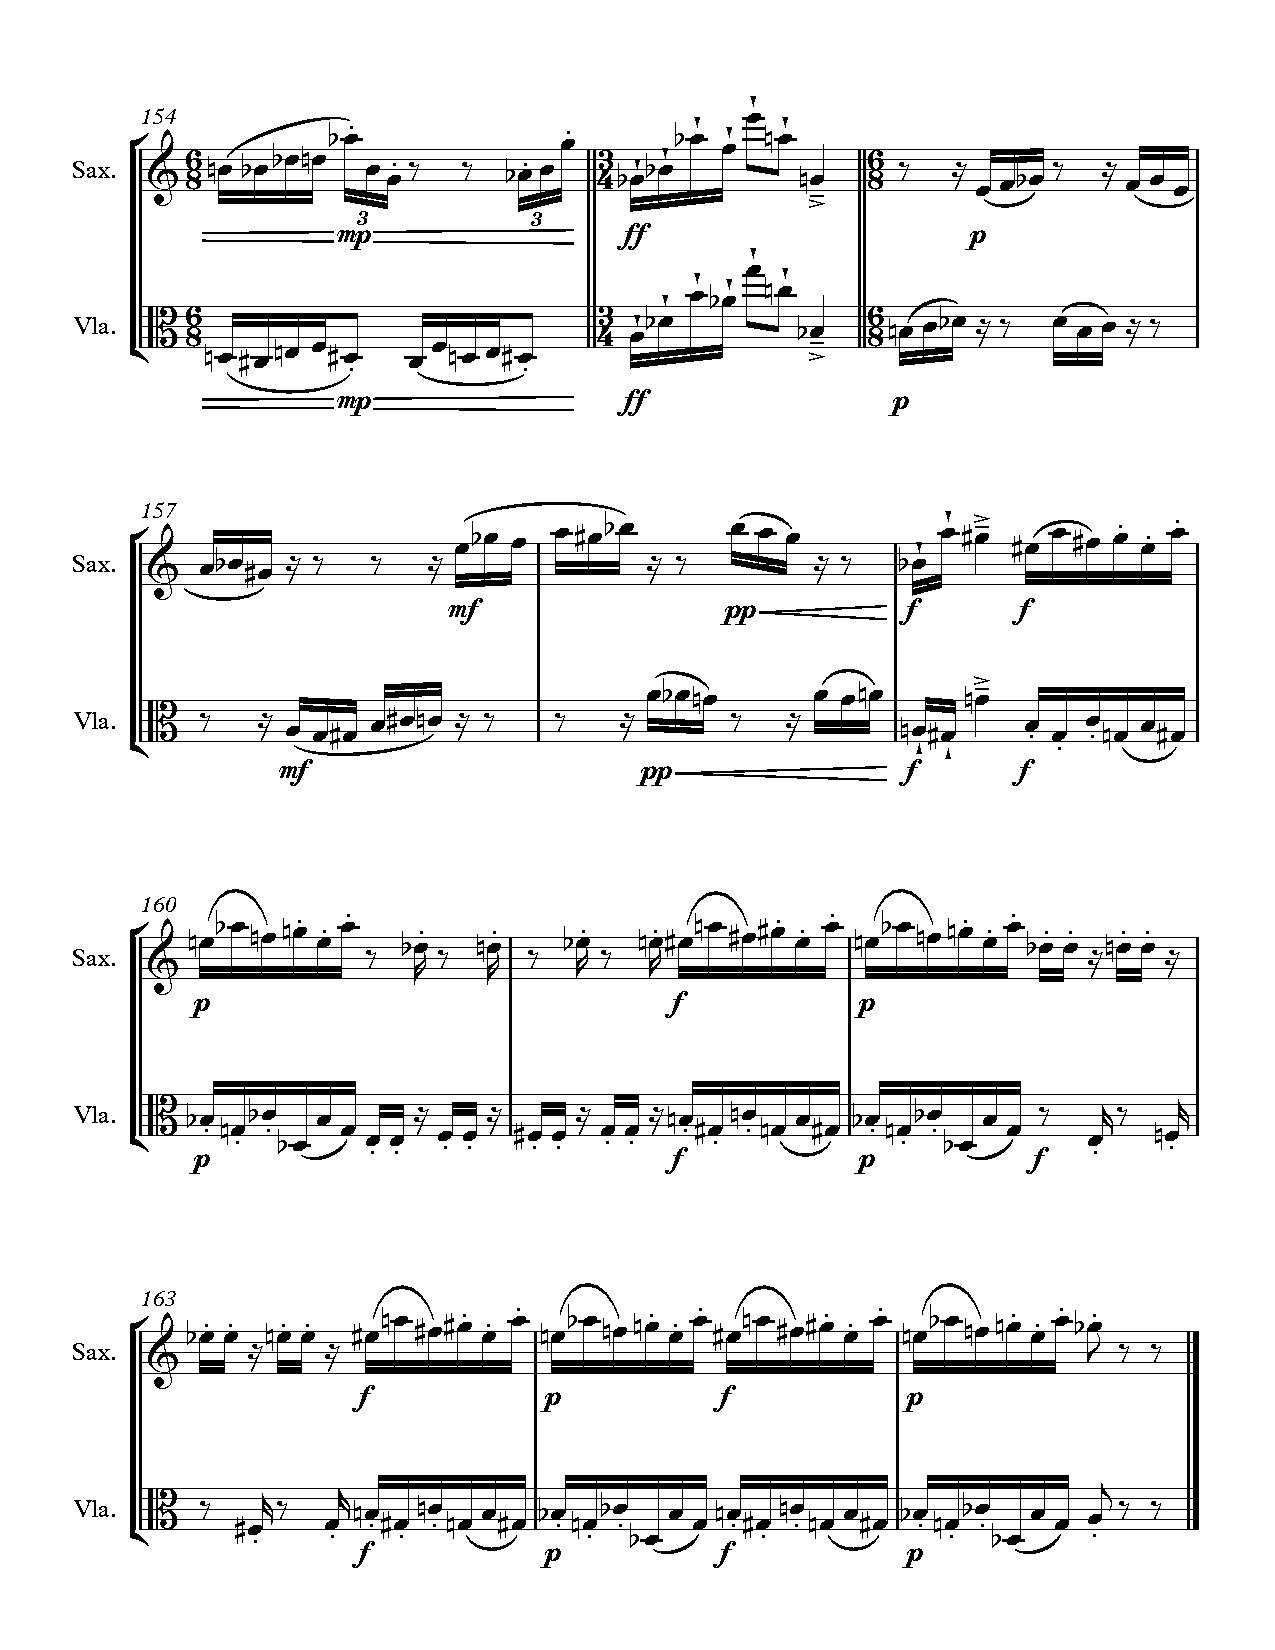
\includegraphics[width=6.5in]{figures/Sax_Viola_14.pdf}
\end{figure}

%--------------------------------------------------------------------------
\begin{figure}[htbp]
    \centering
	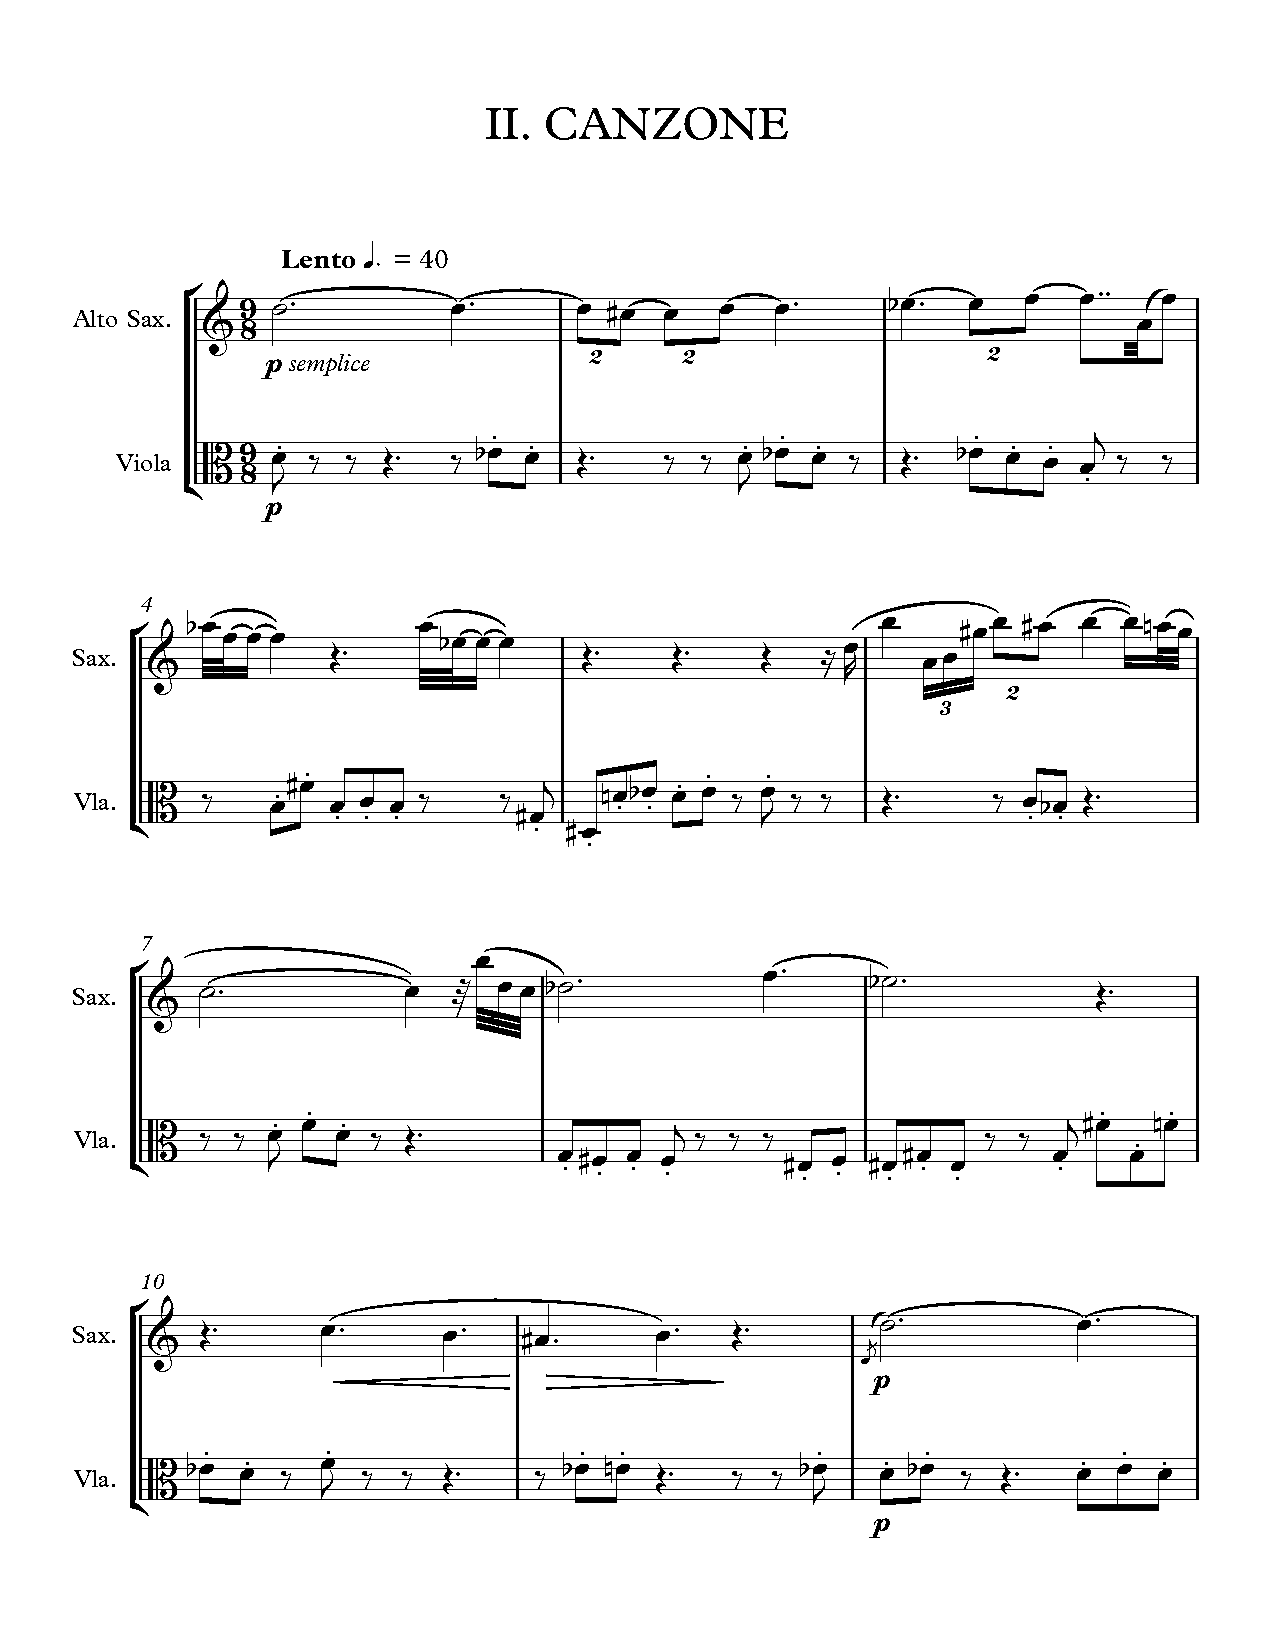
\includegraphics[width=6.5in]{figures/Sax_Viola_15.pdf}
\end{figure}

%--------------------------------------------------------------------------
\begin{figure}[htbp]
    \centering
	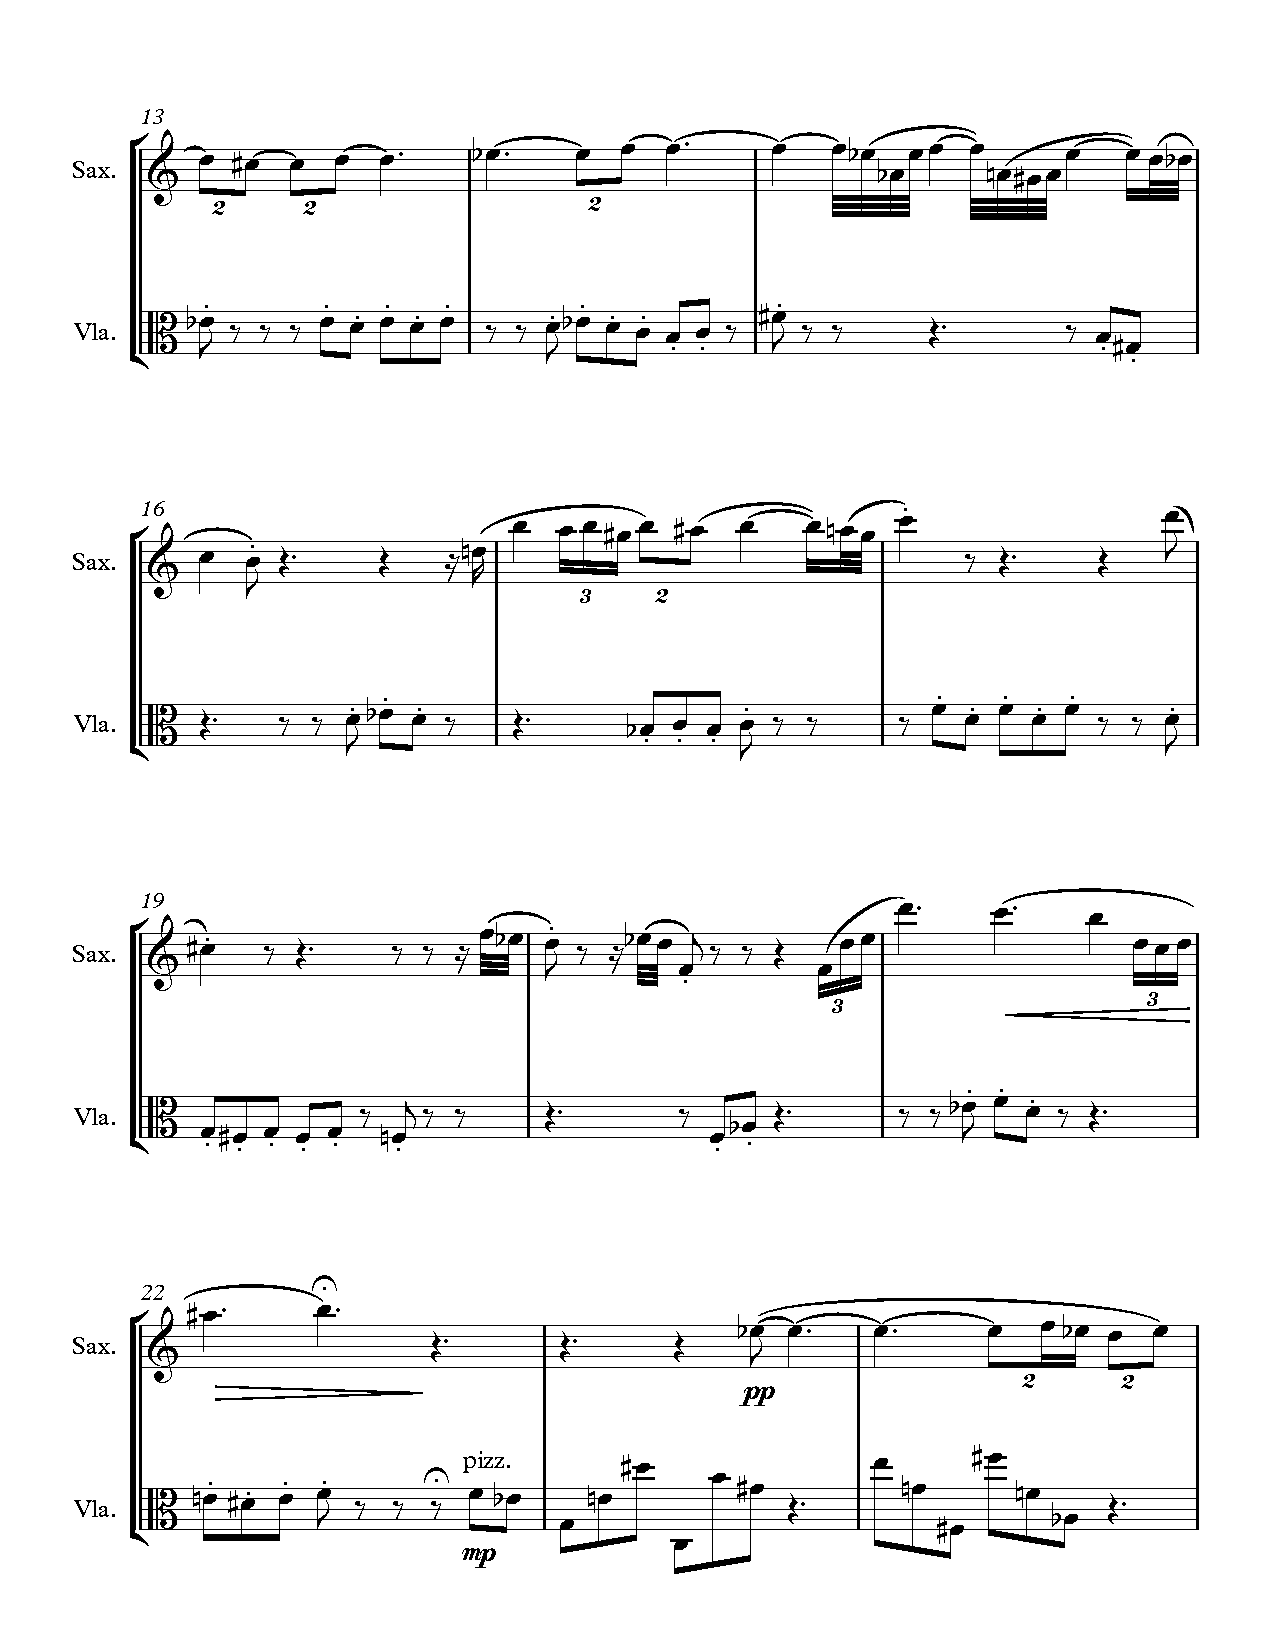
\includegraphics[width=6.5in]{figures/Sax_Viola_16.pdf}
\end{figure}

%--------------------------------------------------------------------------
\begin{figure}[htbp]
    \centering
	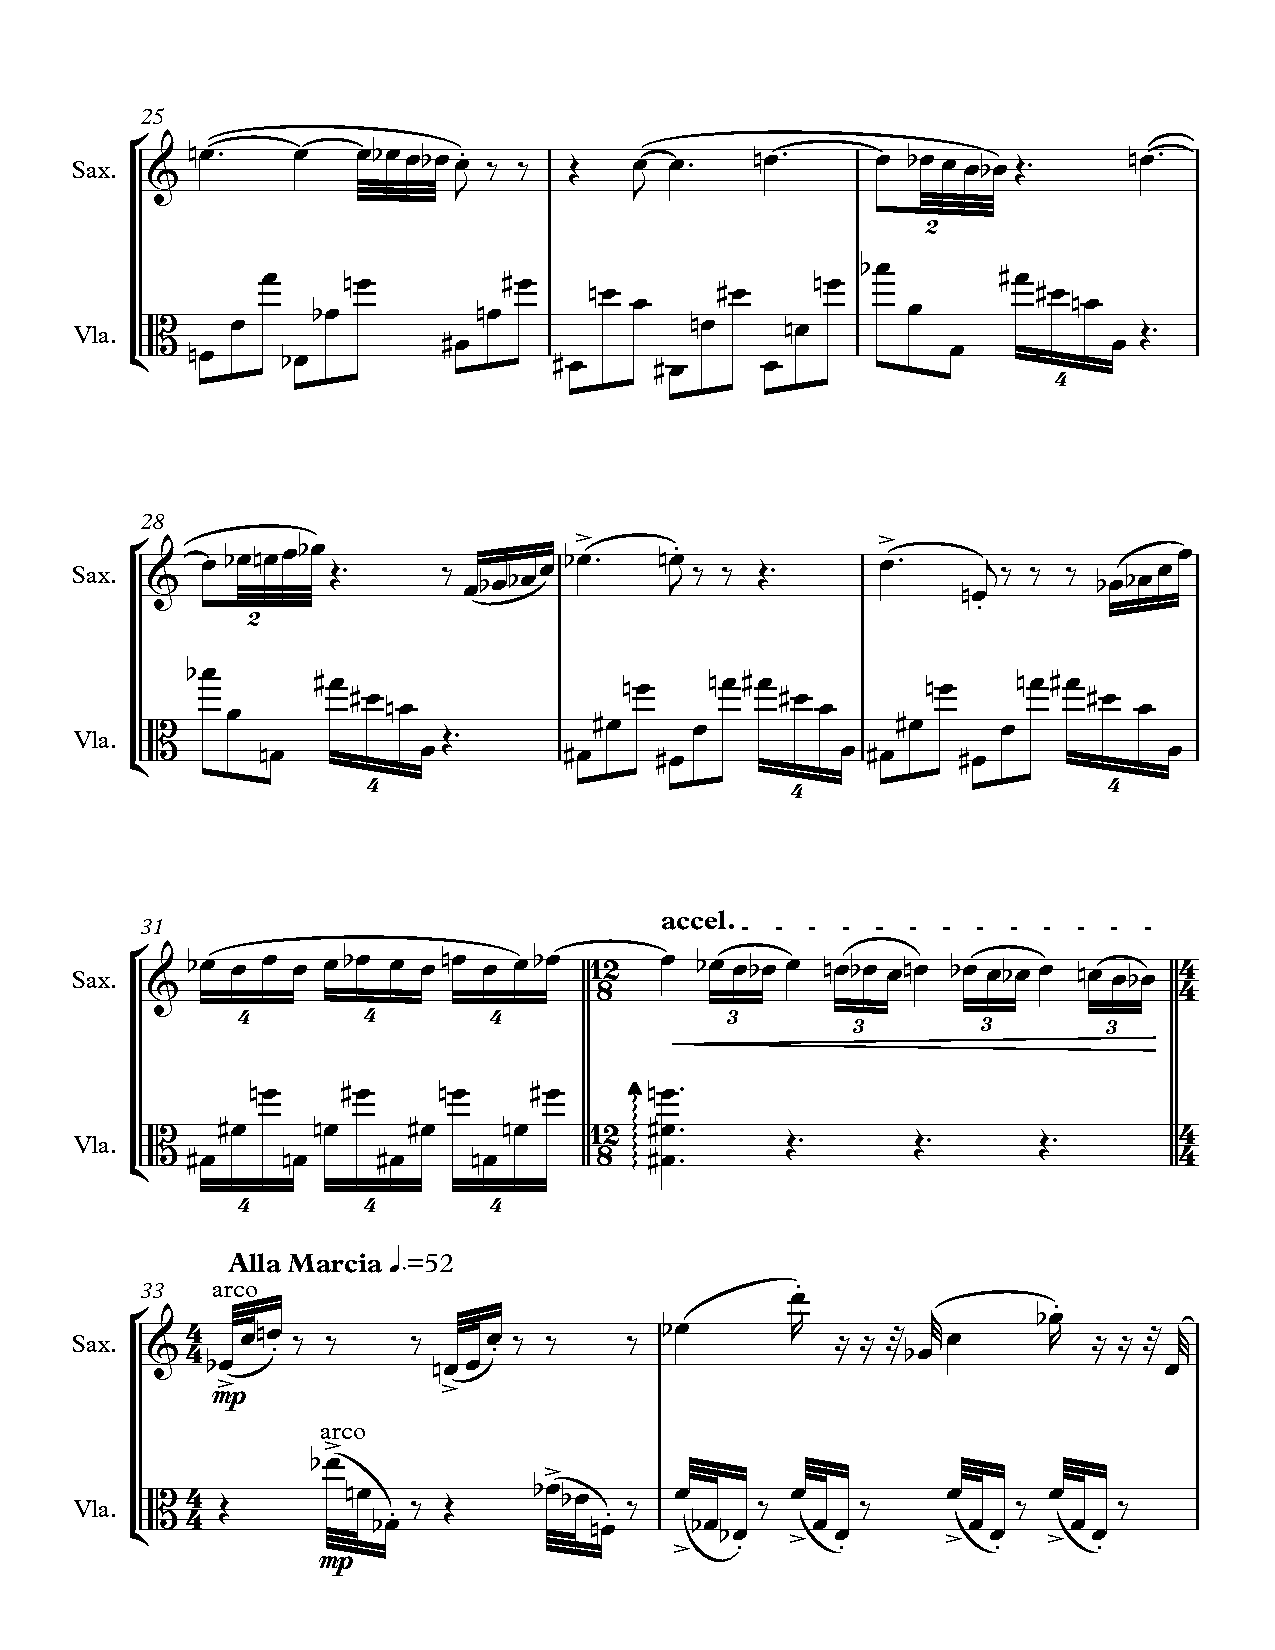
\includegraphics[width=6.5in]{figures/Sax_Viola_17.pdf}
\end{figure}

%--------------------------------------------------------------------------
\begin{figure}[htbp]
    \centering
	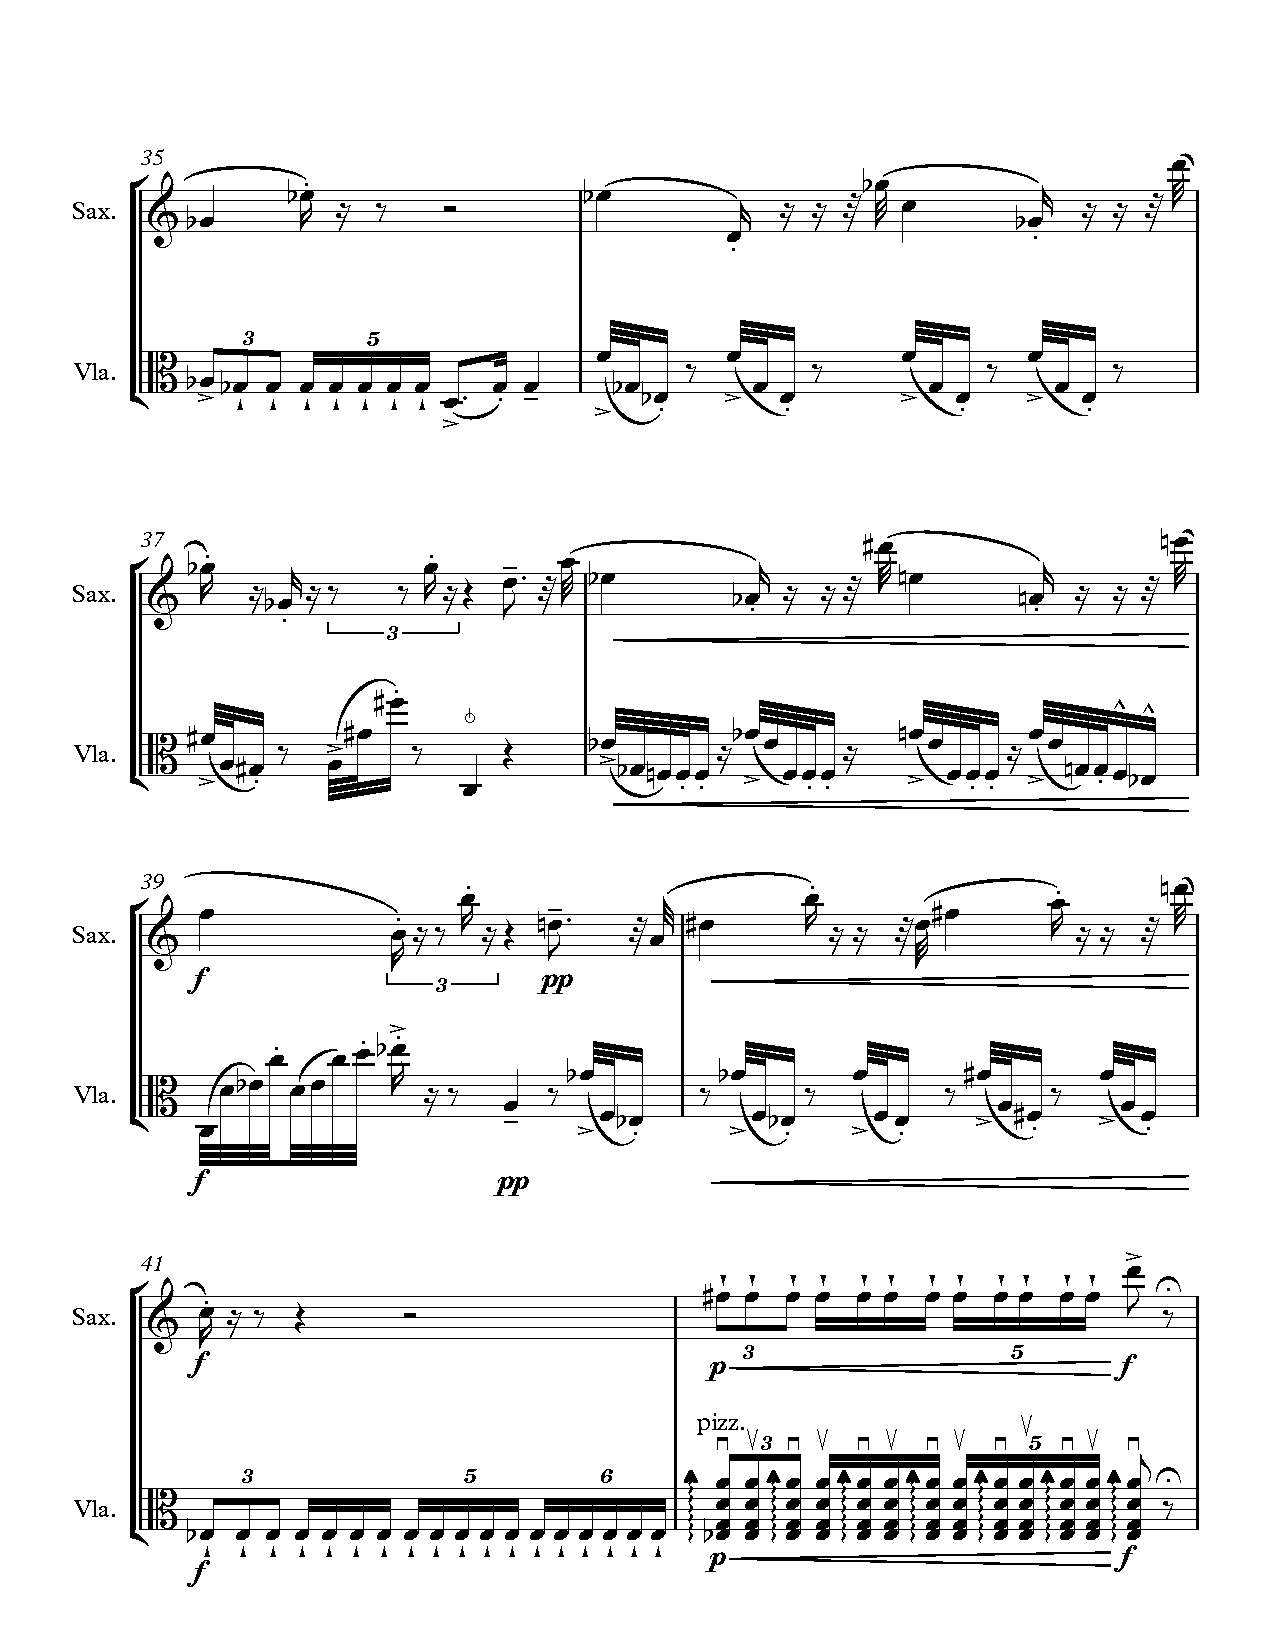
\includegraphics[width=6.5in]{figures/Sax_Viola_18.pdf}
\end{figure}

%--------------------------------------------------------------------------
\begin{figure}[htbp]
    \centering
	\includegraphics[width=6.5in]{figures/Sax_Viola_19.pdf}
\end{figure}

%--------------------------------------------------------------------------
\begin{figure}[htbp]
    \centering
	\includegraphics[width=6.5in]{figures/Sax_Viola_20.pdf}
\end{figure}

%--------------------------------------------------------------------------
\begin{figure}[htbp]
    \centering
	\includegraphics[width=6.5in]{figures/Sax_Viola_21.pdf}
\end{figure}

%--------------------------------------------------------------------------
\begin{figure}[htbp]
    \centering
	\includegraphics[width=6.5in]{figures/Sax_Viola_22.pdf}
\end{figure}

%--------------------------------------------------------------------------
\begin{figure}[htbp]
    \centering
	\includegraphics[width=6.5in]{figures/Sax_Viola_23.pdf}
\end{figure}

%--------------------------------------------------------------------------
\begin{figure}[htbp]
    \centering
	\includegraphics[width=6.5in]{figures/Sax_Viola_24.pdf}
\end{figure}

%--------------------------------------------------------------------------
\begin{figure}[htbp]
    \centering
	\includegraphics[width=6.5in]{figures/Sax_Viola_25.pdf}
\end{figure}

%--------------------------------------------------------------------------
\begin{figure}[htbp]
    \centering
	\includegraphics[width=6.5in]{figures/Sax_Viola_26.pdf}
\end{figure}

%--------------------------------------------------------------------------
\begin{figure}[htbp]
    \centering
	\includegraphics[width=6.5in]{figures/Sax_Viola_27.pdf}
\end{figure}

%--------------------------------------------------------------------------
\begin{figure}[htbp]
    \centering
	\includegraphics[width=6.5in]{figures/Sax_Viola_28.pdf}
\end{figure}

%--------------------------------------------------------------------------
\begin{figure}[htbp]
    \centering
	\includegraphics[width=6.5in]{figures/Sax_Viola_29.pdf}
\end{figure}

%--------------------------------------------------------------------------
\begin{figure}[htbp]
    \centering
	\includegraphics[width=6.5in]{figures/Sax_Viola_30.pdf}
\end{figure}

%--------------------------------------------------------------------------
\begin{figure}[htbp]
    \centering
	\includegraphics[width=6.5in]{figures/Sax_Viola_31.pdf}
\end{figure}

%--------------------------------------------------------------------------
\begin{figure}[htbp]
    \centering
	\includegraphics[width=6.5in]{figures/Sax_Viola_32.pdf}
\end{figure}

%--------------------------------------------------------------------------
\section{Program Notes}

%--------------------------------------------------------------------------
The \emph{Duo for Alto Saxophone and Viola} is written in three movements, all drastically different from one another. The first movement explores the idea of permutation, concentrating almost obsessively on small collections of notes and exhausting their permutational possibilities. On top of this texture, the music unravels in the timbral and dynamical dimensions, producing long-winded phrases. The second movement is a most lyrical song, where the alto saxophone sings freely. The accompaniment is a sculpture \emph{da tirare}, where large blocks of harmony built over Perle-Lansky cycles are trimmed to satisfaction. A middle section is an adaptation of a famous (to some with my background) melody which I shall never reveal. Finally, the third movement is a fugue in which the note collections used for each section are expanding intervallic and rhythmic transforms of the initial statement. In other words, intervals as well as time signatures and motives get bigger up to a certain point, then shrink. Voices are carried and passed back and forth by both instruments, making this a very virtuosic fugue and concluding the piece with fireworks.

%--------------------------------------------------------------------------
\chapter{Duo for Viola and Percussion}

%--------------------------------------------------------------------------
\begin{figure}[h!]
    \centering
	\includegraphics[width=6.5in]{figures/Viola_Percussion_1.pdf}
\end{figure}

%--------------------------------------------------------------------------
\begin{figure}[htbp]
    \centering
	\includegraphics[width=6.5in]{figures/Viola_Percussion_2.pdf}
\end{figure}

%--------------------------------------------------------------------------
\begin{figure}[htbp]
    \centering
	\includegraphics[width=6.5in]{figures/Viola_Percussion_3.pdf}
\end{figure}

%--------------------------------------------------------------------------
\begin{figure}[htbp]
    \centering
	\includegraphics[width=6.5in]{figures/Viola_Percussion_4.pdf}
\end{figure}

%--------------------------------------------------------------------------
\begin{figure}[htbp]
    \centering
	\includegraphics[width=6.5in]{figures/Viola_Percussion_5.pdf}
\end{figure}

%--------------------------------------------------------------------------
\begin{figure}[htbp]
    \centering
	\includegraphics[width=6.5in]{figures/Viola_Percussion_6.pdf}
\end{figure}

%--------------------------------------------------------------------------
\begin{figure}[htbp]
    \centering
	\includegraphics[width=6.5in]{figures/Viola_Percussion_7.pdf}
\end{figure}

%--------------------------------------------------------------------------
\begin{figure}[htbp]
    \centering
	\includegraphics[width=6.5in]{figures/Viola_Percussion_8.pdf}
\end{figure}

%--------------------------------------------------------------------------
\begin{figure}[htbp]
    \centering
	\includegraphics[width=6.5in]{figures/Viola_Percussion_9.pdf}
\end{figure}

%--------------------------------------------------------------------------
\begin{figure}[htbp]
    \centering
	\includegraphics[width=6.5in]{figures/Viola_Percussion_10.pdf}
\end{figure}

%--------------------------------------------------------------------------
\begin{figure}[htbp]
    \centering
	\includegraphics[width=6.5in]{figures/Viola_Percussion_11.pdf}
\end{figure}

%--------------------------------------------------------------------------
\begin{figure}[htbp]
    \centering
	\includegraphics[width=6.5in]{figures/Viola_Percussion_12.pdf}
\end{figure}

%--------------------------------------------------------------------------
\begin{figure}[htbp]
    \centering
	\includegraphics[width=6.5in]{figures/Viola_Percussion_13.pdf}
\end{figure}

%--------------------------------------------------------------------------
\begin{figure}[htbp]
    \centering
	\includegraphics[width=6.5in]{figures/Viola_Percussion_14.pdf}
\end{figure}

%--------------------------------------------------------------------------
\begin{figure}[htbp]
    \centering
	\includegraphics[width=6.5in]{figures/Viola_Percussion_15.pdf}
\end{figure}

%--------------------------------------------------------------------------
\begin{figure}[htbp]
    \centering
	\includegraphics[width=6.5in]{figures/Viola_Percussion_16.pdf}
\end{figure}

%--------------------------------------------------------------------------
\begin{figure}[htbp]
    \centering
	\includegraphics[width=6.5in]{figures/Viola_Percussion_17.pdf}
\end{figure}

%--------------------------------------------------------------------------
\begin{figure}[htbp]
    \centering
	\includegraphics[width=6.5in]{figures/Viola_Percussion_18.pdf}
\end{figure}

%--------------------------------------------------------------------------
\begin{figure}[htbp]
    \centering
	\includegraphics[width=6.5in]{figures/Viola_Percussion_19.pdf}
\end{figure}

%--------------------------------------------------------------------------
\begin{figure}[htbp]
    \centering
	\includegraphics[width=6.5in]{figures/Viola_Percussion_20.pdf}
\end{figure}

%--------------------------------------------------------------------------
\begin{figure}[htbp]
    \centering
	\includegraphics[width=6.5in]{figures/Viola_Percussion_21.pdf}
\end{figure}

%--------------------------------------------------------------------------
\begin{figure}[htbp]
    \centering
	\includegraphics[width=6.5in]{figures/Viola_Percussion_22.pdf}
\end{figure}

%--------------------------------------------------------------------------
\section{Percussion Key}

%--------------------------------------------------------------------------
\begin{figure}[htbp]
    \centering
    \includegraphics[width=6.5in]{figures/Percussion_Key.pdf}
\end{figure}

%--------------------------------------------------------------------------
\section{Program Notes}

%--------------------------------------------------------------------------
The \emph{Duo for Viola and Percussion} is an homage to the \emph{berimbau}, an instrument that was brought from Africa to Brazil, and is a fundamental component of the \emph{capoeira}, a martial art that is drilled as a dance. The piece comprises a single movement with three evolving sections. New motivic seeds are introduced and reintroduced throughout the piece, contributing to a very fluid and energetic atmosphere. Constant technique changes in both instruments evoke the acrobatic ability of the \emph{capoeiristas}, constantly changing roles in a game of capoeira. Besides the actual presence of a berimbau in the percussion setup, the viola also takes up the role of the berimbau through the use of extended techniques, making the piece a true duel filled by music.
